%-----------------------------------------
% To process this file:
%   pdflatex tutorial_bmad_tao
%   bibtex tutorial_bmad_tao
%   pdflatex tutorial_bmad_tao
%   pdflatex tutorial_bmad_tao
%
% IMPORTANT: This file uses .aux files from the Bmad and Tao manuals so pdflatex these manuals beforehand.
%            Note: It is assumed that the bmad, tao, and examples directories are all on the same level.
%-----------------------------------------

\documentclass{hitec}     % Tutorial overall style

\usepackage{index}
\usepackage{xr}
\usepackage{textgreek}
\usepackage{setspace}
\usepackage{graphicx}
\usepackage{moreverb}    % Defines {listing} environment.
\usepackage{amsmath, amsthm, amssymb, amsbsy, mathtools}
\usepackage{alltt}
\usepackage{rotating}
\usepackage{enumitem}
\usepackage{subcaption}
\usepackage{xspace}
%%\usepackage{makeidx}
\usepackage[section]{placeins}   % For preventing floats from floating to end of chapter.
\usepackage{longtable}  % For splitting long vertical tables into pieces
\usepackage{multirow}
\usepackage{booktabs}   % For table layouts
\usepackage{yhmath}     % For widehat
\usepackage{xcolor}      % Needed for listings package.
\usepackage{listings}
\usepackage[T1]{fontenc}   % so _, <, and > print correctly in text.
\usepackage[strings]{underscore}    % to use "_" in text
\usepackage[nottoc,numbib]{tocbibind}   % Makes "References" section show in table of contents
\usepackage[pdftex,colorlinks=true,bookmarksnumbered=true]{hyperref}   % Must be last package!
\usepackage{marginnote}

%----------------------------------------------------------------

\makeatletter   % So can use @ sign in \renewcommand
\renewcommand{\l@subsection}{\@dottedtocline{2}{1.5em}{3.5em}}
\makeatother    % Reset 

%\definecolor{cverbbg}{gray}{0.93}
\definecolor{cverbbg}{rgb}{0.95,0.95,0.92}


% This makes margin notes aways appear on the same side

\makeatletter
\renewcommand{\l@subsection}{\@dottedtocline{2}{1.5em}{3.5em}}
\patchcmd{\@mn@@@marginnote}{\begingroup}{\begingroup\@twosidefalse}{}{\fail}
\reversemarginpar
\makeatother

%

\newcommand{\Bf}[1]{{\bf #1}}
\newcommand{\dsfrac}[2]{\frac{\displaystyle #1}{\displaystyle #2}}
\newcommand{\calO}{{\cal O}}
\newcommand{\calH}{{\cal H}}
\newcommand{\Cal}[1]{{\cal #1}}
\newcommand{\two}{}
\newcommand{\bfsig}{\boldsymbol{\sigma}}
\newcommand{\bfbeta}{\boldsymbol{\beta}}
\newcommand{\bfphi}{\boldsymbol{\phi}}
\newcommand{\bfeta}{\boldsymbol{\eta}}
\newcommand{\sigb}{\sigma_\beta}
\newcommand{\bfrbar}{\overline{\Bf r}}
\newcommand{\BF}[1]{{\text{\bf #1}}}
%%\newcommand{\BF}[1]{{\normalfont\textbf{#1}}}

\newcommand{\re}{\operatorname{Re}}
\newcommand{\im}{\operatorname{Im}}

\newcommand{\bfa}{\Bf a}
\newcommand{\bfg}{\Bf g}
\newcommand{\bfk}{\Bf k}
\newcommand{\bfq}{\Bf q}
\newcommand{\bfr}{\Bf r}
\newcommand{\bfx}{\Bf x}
\newcommand{\bfz}{\Bf z}
\newcommand{\bfA}{\Bf A}
\newcommand{\bfB}{\Bf B}
\newcommand{\bfC}{\Bf C}
\newcommand{\bfE}{\Bf E}
\newcommand{\bfG}{\Bf G}
\newcommand{\bfH}{\Bf H}
\newcommand{\bfI}{\Bf I}
\newcommand{\bfL}{\Bf L}
\newcommand{\bfM}{\Bf M}
\newcommand{\bfO}{\Bf O}
\newcommand{\bfQ}{\Bf Q}
\newcommand{\bfK}{\Bf K}
\newcommand{\bfP}{\Bf P}
\newcommand{\bfR}{\Bf R}
\newcommand{\bfS}{\Bf S}
\newcommand{\bfV}{\Bf V}
\newcommand{\bfT}{\Bf T}
\newcommand{\bfU}{\Bf U}
\newcommand{\bfW}{\Bf W}

\newcommand{\vdot}[2]{\Bigl[ #1, \, #2 \Bigr]}
\newcommand{\comma}{\> ,}
\newcommand{\period}{\> .}
\newcommand{\bfAbar}{\overline{\bfA}}
\newcommand{\bfCbar}{\overline{\bfC}}
\newcommand{\bfKbar}{\overline{\bfK}}
\newcommand{\bfkbar}{\overline{\bfk}}
\newcommand{\bfTbar}{\overline{\bfT}}
\newcommand{\Hbar}{{\overline{H}}}
\newcommand{\Kbar}{\overline{K}}
\newcommand{\kbar}{\overline{k}}
\newcommand{\Pbar}{\overline{P}}
\newcommand{\gam}{\gamma}                                     
\newcommand{\inv}{^{-1}}

\newcommand{\tot}{{\text{tot}}}

%%\newcommand{\dotproduct}{\mathbin{\scriptscriptstyle\stackrel{\bullet}{{}}}}
\newcommand{\dotproduct}{\mathbin{\boldsymbol{\cdot}}}
\newcommand{\cross}{\mathbin{\boldsymbol{\times}}}

\newcommand{\what}{\widehat}
\newcommand{\wt}{\widetilde}
\newcommand{\bfhat}[1]{{\widehat{\bf  #1}}}
\newcommand{\bftilde}[1]{{\widetilde{\bf #1}}}
\newcommand{\xw}{{\widetilde x}}
\newcommand{\yw}{{\widetilde y}}
\newcommand{\rw}{{\widetilde r}}

\newcommand{\tstyle}{\textstyle}
\newcommand{\stilde}{{\widetilde s}}
\newcommand{\tWl}{\widetilde{W}^{SR}_\parallel}
\newcommand{\WlS}{W^{SR}_\parallel}
\newcommand{\WtS}{W^{SR}_\perp}
\newcommand{\WtL}{W^{LR}_\perp}

\newcommand{\hyperbf}[1]{\textbf{\hyperpage{#1}}}
\newcommand{\Hyperref}[2]{\index[routine]{#2}\hyperref[#1]{#2}}

\newcommand{\om}{\omega}
\newcommand{\qqquad}{\qquad \qquad}
\newcommand{\ks}{\widetilde k_s}
\newcommand{\kone}{\widetilde k_1}

\newcommand{\hphphp}{\hphantom{\dfrac{k_x}{k_y}}}
\newcommand{\Ce}{\text{C}}
\newcommand{\Se}{\text{S}}
\newcommand{\Ch}{\text{Ch}}
\newcommand{\Sh}{\text{Sh}}

\newcommand{\CR}{\\}
\newcommand{\CRNO}{\nonumber \\}
\newcommand{\dstyle}{\displaystyle}

\newcommand{\fig}[1]{Fig.~\ref{#1}}
\newcommand{\figs}[1]{Figs.~\ref{#1}}

\newcommand{\pow}[1]{\cdot 10^{#1}}
\newcommand{\tao}{{\sl Tao}\xspace}
\newcommand{\ltt}{{\sl Long Term Tracking}\xspace}
\newcommand{\da}{{\sl Dynamic Aperture}\xspace}
\newcommand{\sodom}{{\sl SODOM-2}\xspace}
\newcommand{\spinstrob}{{\sl spin_stroboscope}\xspace}
\newcommand{\bmad}{{\sl Bmad}\xspace}
\newcommand{\mad}{{\sl MAD}\xspace}
\newcommand{\quickplot}{{\sl Quick Plot}\xspace}
\newcommand{\cpp}{$C$\hskip-0.3ex\protect\raisebox{0.2ex}{\scriptsize ++}\xspace}
\newcommand{\CPP}{$C$\hskip-0.3ex{\protect\raisebox{.3ex}{\large {+}+}}\xspace}
%%\newcommand{\CPP}{$C${\small ++}\xspace}

\newcommand{\eq}[1]{{(\protect\ref{#1})}}
\newcommand{\Eq}[1]{{Eq.~(\protect\ref{#1})}}
\newcommand{\Eqs}[1]{{Eqs.~(\protect\ref{#1})}}

\newcommand{\svn}{\vn{Subversion}\xspace}
\newcommand{\sref}[1]{\S\ref{#1}}
\newcommand{\Sref}[1]{Sec.~\sref{#1}}
\newcommand{\extref}[1]{\S\ref*{#1}}   % No hyperlink. For external refs. \extref
\newcommand{\cref}[1]{Chapter~\ref{#1}}

\newcommand{\toffset}{\vskip 0.01in}
\newcommand{\rot}[1]{\begin{rotate}{-45}#1\end{rotate}}

\newcommand{\ave}[1]{\left\langle #1 \right\rangle}

\newcommand{\vn}{\begingroup\catcode`\_=11 \catcode`\%=11 \dottcmd}
\newcommand\dottcmd[1]{{\usefont{T1}{lmss}{bx}{n} #1}\endgroup}

%\newcommand\ttverb{
%  \bgroup\let\do\@makeother\dospecials\catcode`{=1 \catcode`}=2 \DSAcode}
%\newcommand*\DSAcode[1]{\texttt{#1}\egroup}

\newcommand{\CRNEG}{\nonumber \\*[-1.5\jot]}
\newcommand{\CRneg}{\nonumber \\*[-1\jot]}
\newcommand{\Newline}{\hfil \\}

\newcommand{\plus}{\; + \;}

\newcommand{\Th}{$^{th}$\xspace}
\newcommand{\Nd}{$^{nd}$\xspace}
\newcommand{\Rd}{$^{rd}$\xspace}
\newcommand{\St}{$^{st}$\xspace}
\newcommand{\B}{$\backslash$}

\newlength{\dPar}
\setlength{\dPar}{1.5ex}

% Since a non-zero parskip is used, the alltt environment needs to be modified to keep
% the white space before and after from being too large.

% Note: Use \( ... \) for inline equations in example mode. 
% Use \[ ... \] for display equations.
%\sb{} and \sp{} need to be used for subscripts and superscripts instead of "_" and "^".

\newenvironment{example}
  {\vspace{-3.0ex} \begin{alltt}}
  {\end{alltt} \vspace{-2.5ex}}

\newenvironment{example2}
  {\vspace{-2.5ex} \begin{alltt}}
  {\end{alltt} \vspace{-2.0ex}}

\newenvironment{Itemize}
  {\begin{list}{$\bullet$}
    {\addtolength{\topsep}{-1.5ex} 
     \addtolength{\itemsep}{-1ex}
    }
  }
  {\end{list} \vspace*{1ex}}

\definecolor{light-gray}{gray}{0.95}
\lstset{backgroundcolor=\color{light-gray}}
\lstset{xleftmargin=0cm}
\lstset{framexleftmargin=0.3em}

\lstnewenvironment{Xcode}{}{}

%\definecolor{lightcyan}{rgb}{0.945, 0.945, 0.945}
\definecolor{lightcyan}{rgb}{0.999, 0.97, 0.94}
\newcounter{main}
\setcounter{main}{1}

\lstnewenvironment{code}[1][firstnumber=\themain,name=main]
  {\lstset{ %language=haskell,
           %columns=fullflexible,
           columns=fixed,
           basicstyle=\footnotesize,
           %numbers=left,
           numberstyle=\tiny\color{gray},
           backgroundcolor=\color{lightcyan},
           #1
          }
}
{\setcounter{main}{\value{lstnumber}}}

%\newenvironment{code}
% {\SaveVerbatim{cverb}}
% {\endSaveVerbatim
%  \flushleft\fboxrule=0pt\fboxsep=.5em
%  \colorbox{cverbbg}{%
%    \makebox[\dimexpr\linewidth-2\fboxsep][l]{\BUseVerbatim{cverb}}%
%  }
%  \endflushleft
%}


{\setcounter{main}{\value{lstnumber}}}

% \ExampleNum is for numbering "example" blocks using the same numbering counter
% as the "equation" counter

\newcommand{\ExampleNum}[1]{\hfill \refstepcounter{equation} \((\arabic{equation})\protect\label{#1}\)}

% From pg 64 of The LaTex Companion.

\newenvironment{ventry}[1]
  {\begin{list}{}
    {\renewcommand{\makelabel}[1]{\textsf{##1}\hfil}
     \settowidth{\labelwidth}{\textsf{#1}}
     \addtolength{\itemsep}{-1.5ex}
     \addtolength{\topsep}{-1.0ex} 
     \setlength{\leftmargin}{5em}
    }
  }
  {\end{list}}

\newcommand{\BAR}[1]{\overline{#1}}

\newcommand{\DAG}{$^\dagger$}
\newcommand{\DDAG}{$^\ddagger$}

%Units in roman
\newcommand{\unit}[1]{\,\ensuremath{\mathrm{#1}}}




% These are used with \extref

\externaldocument[T-]{../../../tao/doc/command-list}
\externaldocument[T-]{../../../tao/doc/data}
\externaldocument[T-]{../../../tao/doc/initialization}
\externaldocument[T-]{../../../tao/doc/introduction}
\externaldocument[T-]{../../../tao/doc/wave}
\externaldocument[T-]{../../../tao/doc/overview}
\externaldocument[T-]{../../../tao/doc/optimization}
\externaldocument[B-]{../../../bmad/doc/elements}
\externaldocument[B-]{../../../bmad/doc/lattice-file}
\externaldocument[B-]{../../../bmad/doc/lines-and-lists}

\renewcommand{\ttdefault}{txtt}
%\lstset{basicstyle = \small\asciifamily,columns=flexible}  % Enable cut and paste
\definecolor{backcolor}{rgb}{0.8824,1.0,1.0}   % To match code environment
\lstset{basicstyle = \small, backgroundcolor=\color{backcolor}, escapeinside = {@!}{!@}}

\renewcommand{\textfraction}{0.1}
\renewcommand{\topfraction}{1.0}
\renewcommand{\bottomfraction}{1.0}

\settextfraction{0.9}  % Width of text
\setlength{\parindent}{0pt}
\setlength{\parskip}{1ex}
%\setlength{\textwidth}{6in}
\newcommand{\Section}[1]{\section{#1}\vspace*{-1ex}}

\newenvironment{display}
  {\vspace*{-1.5ex} \begin{alltt}}
  {\end{alltt} \vspace*{-1.0ex}}

\title{An Introduction and Tutorial to Bmad and Tao}
\author{}
\date{David Sagan and Chris Mayes \\ July 4, 2025}

\begin{document}

\phantomsection
\pdfbookmark[1]{Cover Page}{Cover Page}
\maketitle

\cleardoublepage
\phantomsection
\pdfbookmark[1]{Contents}{Contents}
\tableofcontents

\newpage

%------------------------------------------------------------------------------
%------------------------------------------------------------------------------
\Section{A Guide for the Perplexed}
\label{s:guide}

This tutorial is a guide to introduce the reader to the \bmad toolkit for relativistic
charged--particle and X-Ray simulations. Additionally, this tutorial serves as an introduction
to \tao which is a simulation program based upon the \bmad toolkit.

It is assumed that you know something about accelerator physics. For example, it is assumed that
\reversemarginpar\marginpar{\raggedleft\includegraphics[width=40pt]{maimonides.pdf}\vspace*{10pt}}
you know something about beta functions, dispersion and closed orbits. It is also assumed that
you are familiar with the basics of Unix and how to use a command line interface.

%------------------------------------------------------------------------------
\subsection{Overview: What is Bmad? What is Tao?}
\label{s:overview}

\begin{description}
%
\marginnote{\footnotesize\hspace*{-0.4in}\parbox{0.95in}{
Only the first letter of \bmad is capitalized. the rest is lower case.
}}[0.1in]
%
\item[Bmad] \Newline
\bmad is an ecosystem of toolkits (software libraries) and programs for the simulation of charged
particles and X-rays. At the heart of this ecosystem is the open source \bmad toolkit which can be
used to construct simulation programs in less time and with fewer bugs than can be done from
scratch. There is some ambiguity here since the name \bmad can refer to the entire ecosystem in
general or the \bmad toolkit in particular. Generally the context will make things clear.

Over the years, \bmad has been used for a wide range of charged-particle and X-ray simulations. This
includes:
\begin{code}
Lattice design                                  X-ray simulations
Spin tracking                                   Wakefields and HOMs
Beam breakup (BBU) simulations in ERLs          Touschek Simulations
Intra-beam scattering (IBS) simulations         Dark current tracking
Coherent Synchrotron Radiation (CSR)            Frequency map analysis
\end{code}
%
\item[Tao] \Newline
\tao is a general purpose simulation program, based upon the \bmad toolkit. \tao can be used to view
lattices, do Twiss and orbit calculations, nonlinear optimization on lattices, etc., etc.
Additionally, \tao's object oriented design makes it relatively easy to extend it. For example, it
can be used for orbit flattening in an online machine control system.
  \end{description}

%------------------------------------------------------------------------------
\subsection{How to use this Tutorial!}
\label{s:use.tutorial}

This tutorial is meant to be \vn{``hands on''}. That is, you should be \vn{using Tao} as you read
through the chapters. Additionally, it is \vn{expected} (nay, \vn{necessary}) that you \vn{consult}
the \vn{Bmad} and \vn{Tao} manuals for information on topics that are only partially covered in this
tutorial (and in fact, the exercises at the ends of the tutorial chapters are meant to motivate
further reading of the manuals).

\newpage

%------------------------------------------------------------------------------
%------------------------------------------------------------------------------
\Section{Orientation}
\label{s:orientation}

%------------------------------------------------------------------------------
\subsection{Web Site}

The \bmad web site is at:
\begin{display}
  \url{\detokenize{www.classe.cornell.edu/bmad/}}
\end{display}
Here you will find documentation on the \bmad toolkit and associated programs as well as
installation instructions.

%------------------------------------------------------------------------------
\subsection{Prerequisites}

\bmad and \tao can be run under Linux, Mac OS-X, or Windows running Windows Subsystem for Linux 2 (WSL2)
which allows running in a Linux environment on Windows.

Except when using a Python interface, \tao is accessed through the command line.  Therefore you will
need to run a terminal program to be able to run \tao.

%------------------------------------------------------------------------------
\subsection{Bmad Slack Workspace}

There is a Slack workspace for \bmad. This workspace is a valuable resource if you have
questions about anything related to \bmad and \tao. Sign up is at:
\begin{display}
  \url{\detokenize{join.slack.com/t/bmad-simulation/shared_invite/zt-flwsmsc3-ITpqJyhRKNwWkZSA6b4LUw}}
\end{display}
This link allows you to sign up if you have a recognized email domain. If you do not, please contact
a \bmad maintainer (click the ``Help'' button in the \bmad web site) and an invitation can be
issued.

%------------------------------------------------------------------------------
\subsection{Minimum Bmad/Tao Version Compatible with Tutorial}

This tutorial can be used with any version of \bmad and \tao dated July 12, 2020 or after
(\sref{s:orientation}). For versions of \bmad and \tao before this, some difficulties may be
encountered.

%------------------------------------------------------------------------------
\subsection{Tao Executable Installation}
\label{s:install}

If you have a local \bmad Guru, check with you Guru to see if there is a \tao executable that you
can use which will save you the trouble of installing one.

Installation instructions are posted on the \bmad web site.
There are two possible routes. One possibility is to use \vn{Conda-forge} (a Python
package manager) to download a \tao executable. The other is to compile a \bmad Release from GitHub
(\sref{s:dist}).

Even if you do use \vn{Conda}, you should also download (but you do not need to compile) a
Release (\sref{s:dist}) since a Release contains many useful lattice examples.

If you compile a \vn{Release}, a useful check that everything is setup
is the \vn{accinfo} command which shows the environment variables that have been setup by the
compile scripts.
\begin{code}
> accinfo

DIST_DEBUG=/Users/dcs16/Bmad/bmad_dist_2020_0712-0/debug/bin
DIST_OS=Darwin
DIST_BUILD=TRUE
DIST_F90=gfortran
DIST_UTIL=/Users/dcs16/Bmad/bmad_dist_2020_0712-0/util
DIST_BASE_DIR=/Users/dcs16/Bmad/bmad_dist_2020_0712-0
... etc...
ACC_EXE=/Users/dcs16/Bmad/bmad_dist_2020_0712-0/production/bin
ACC_CMAKE_VERSION=2.8.5
ACC_DEBUG=/Users/dcs16/Bmad/bmad_dist_2020_0712-0/debug/bin
ACC_BUILD_SYSTEM=/Users/dcs16/Bmad/bmad_dist_2020_0712-0/build_system
ACC_PLOT_DISPLAY_TYPE=X
... etc...
\end{code}
One common mistake, if you have multiple Releases on your system, is having the environment
variables pointing to a Release other than the one you want to use. The \vn{accinfo} command
is a quick way to tell if there is a problem.

%------------------------------------------------------------------------------
\subsection{Releases}
\label{s:dist}

A \vn{Release}, hosted on GitHub, is a set of files, including \bmad and \tao source files, which
are used to build the \bmad, the \tao program, and various other simulation programs.

The directories in a Release are:
\begin{lstlisting}[mathescape]
INSTALL             fftw                lattice            regression_tests
PGPLOT              fgsl                lux                sim_utils
bmad                bmad-doc            forest             mad_tpsa
tao                 bsim                gnu_utilities_src  open_spacecharge
util                build_system        gsl                openmpi
util_programs       cpp_bmad_interface  hdf5               plplot
xraylib             examples            lapack             xsif
\end{lstlisting}

For an explanation of what directories contain what, see:
\begin{display}
  \url{https://wiki.classe.cornell.edu/ACC/ACL/OffsiteDoc#DistDirs}
\end{display}

\newpage

%------------------------------------------------------------------------------
%------------------------------------------------------------------------------
\Section{Resources}
\label{s:resources}

More information is readily available at the \bmad web site:
\begin{display}
  \url{\detokenize{www.classe.cornell.edu/bmad/}}
\end{display}
Links to the most up-to-date \bmad and \tao manuals can be found there as well as manuals for other
programs and instructions for downloading and setup. The manuals are at:
\begin{display}
  \url{\detokenize{www.classe.cornell.edu/bmad/bmad-manual.pdf}}
  \url{\detokenize{www.classe.cornell.edu/bmad/tao-manual.pdf}}
\end{display}

This tutorial, along with associated lattice files and other examples may be obtained from \vn{GitHub}
(\sref{s:orientation})
\begin{lstlisting}[mathescape]
  \url{github.com/bmad-sim/bmad-doc}
\end{lstlisting}

To keep in touch with the latest \bmad developments, there are two mailing lists for
\bmad.  The \vn{bmad-l} mailing list is used to send information on Bmad developments.  The
\vn{bmad-devel-l} mailing list is for programmers. The volume of e-mail is small -- Typically
less than one a week. Instructions on how to sign up can be obtained from the \bmad web
page.

%------------------------------------------------------------------------------
\subsection{Bmad Directories}
\label{s:bmad.dir}

A quick introduction to the most important directories in a \vn{Release}:
\begin{description}
%
\vspace{-0.4 ex}
\item[bmad] \Newline
The \vn{bmad} directory holds the code for the \bmad library.
%
\vspace{-0.4 ex}
\item[bsim] \Newline
The \vn{bsim} directory holds the code for some \bmad based programs for simulating
synchrotron radiation (programs: \vn{synrad} and \vn{synrad3d}), dynamic_aperture (program:
\vn{dynamic_aperture}), intra-beam scattering (programs: \vn{ibs_linac} and \vn{ibs_ring}), etc.
%
\vspace{-0.4 ex}
\item[debug] \Newline
The \vn{debug} directory is like the \vn{production} directory except that the executables in the
\vn{debug/bin} directory have been compiled with the \vn{debug} flag. These executables can be used
with a debugger but, since they typically run much slower than their counterparts in
\vn{production/bin}, these executables should not be used for normal running.
%
\vspace{-0.4 ex}
\item[examples] \Newline
The \vn{examples} directory holds example programs.
%
\vspace{-0.4 ex}
\item[production] \Newline
The \vn{production} directory is created when the code in a \vn{Release} is
compiled. It contains various libraries, modules, and other files. In particular, the
\vn{production/bin} directory contains executable files for \tao and other \bmad based simulation
programs. Note: Many directories will themselves contain a \vn{production} directory. For example,
there will be a \vn{bmad/production} and a \vn{tao/production} directory. Do not confuse these
directories with the top level \vn{production} directory. The second tier production directories do
not contain anything of interest.
%
\vspace{-0.4 ex}
\item[tao] \Newline
The \vn{tao} directory holds the code for the \tao program as well as example input
files in the \vn{bmad-doc/tao_examples/} directory.
%
\vspace{-0.4 ex}
\item[util] \Newline
The \vn{util} directory holds various build scripts.
%
\vspace{-0.4 ex}
\item[util_programs] \Newline
The \vn{util_program} directory holds the code for various utility programs including programs for
converting between \bmad lattice files to other formats (MAD, SAD, etc.).

\end{description}

\newpage

%------------------------------------------------------------------------------
%------------------------------------------------------------------------------
\Section{Bmad Based Programs}
\label{s:programs}

Below is a partial list of simulation and helper programs that are based upon \bmad. All of these
programs are included in any \vn{Release}. The program executable will be in
the \vn{production/bin} directory (\sref{s:bmad.dir}).

Documentation for some of the program can be found at:
\begin{display}
  \url{www.classe.cornell.edu/bmad/other_manuals.html}
\end{display}
Example input files, along with documentation source files and other information, can generally be
found in the directory that holds the source code as noted below.

Note: Before running any program, the appropriate environment variables must be setup. [The setup
for running programs and the setup for compiling \bmad based programs is one and the same.] Ask your
local \bmad guru about this or consult the \bmad web page (\sref{s:resources}) for directions.

  \begin{description}
%
  \item[bmad_to_mad_and_sad] \Newline
The \vn{bmad_to_mad_and_sad} program converts \bmad lattice format files to \vn{MAD8}, \vn{MADX} and
\vn{SAD} format.
%
  \item[bbu] \Newline
The \vn{bbu} program simulates the beam breakup instability in Energy Recovery Linacs (ERLs). The
source code is in the directory \vn{bsim/bbu}.
%
  \item[dynamic_aperture] \Newline
The \vn{dynamic_aperture} program finds the dynamic aperture through tracking. The source code is in
the \vn{bsim/dynamic_aperture} directory.
%
  \item[ibs_linac] \Newline
The \vn{ibs_linac} program simulates the effect of intra-beam scattering (ibs) for beams
in a Linac. The source code is in the \vn{bsim/ibs_linac} directory.
%
  \item[ibs_ring] \Newline
The \vn{ibs_linac} program simulates the effect of intra-beam scattering (ibs) for beams
in a ring. The source code is in the \vn{bsim/ibs_linac} directory.
%
  \item[long_term_tracking] \Newline
The \vn{long_term_tracking_program} is for long term tracking of a particle or beam possibly
including tracking of the spin.
%
  \item[lux] \Newline
The \vn{lux} program simulates X-ray beams from generation through to experimental end stations.
The source code is in the \vn{lux} directory.
%
  \item[mad8_to_bmad.py, madx_to_bmad.py] \Newline
These python programs will convert \vn{MAD8} and \vn{MADX} lattice files to to \bmad format. The
scripts are in the \vn{util_program/mad_to_bmad} directory
%
  \item[synrad] \Newline
The \vn{synrad} program computes the power deposited on the inside of a vacuum chamber
wall due to synchrotron radiation from a particle beam. The calculation is essentially two
dimensional but the vertical emittance is used for calculating power densities along the
centerline. Crotch geometries can be handled as well as off axis beam orbits. The source code 
is in the \vn{bsim/synrad} and \vn{bsim/code_synrad} directories. 
%
  \item[synrad3d] \Newline
The \vn{synrad3d} program tracks, in three dimensions, photons generated from a beam
within the vacuum chamber. Reflections at the chamber wall is included. Source code is
in the \vn{bsim/synrad3d} and \vn{bsim/code_synrad3d} directories.
%
  \item[tao] \Newline
\tao is a general purpose simulation program described in \sref{s:overview}. The source code can be
found in the \vn{tao} directory. Documentation is available from the web (\sref{s:resources}).
%
  \item[tune_scan] \Newline
The \vn{tune_scan} program produces data for plotting resonances in the transverse $(Q_a, Q_b)$ tune
plane.  This is done by adjusting the lattice tunes $Q_a$ and $Q_b$ to some values and then tracking
a beam of particles while recording various parameters like the beam size. This is done repeatedly
on a grid of points in the $(Q_a, Q_b)$ tune plane.
  \end{description}

\newpage

%------------------------------------------------------------------------------
%------------------------------------------------------------------------------
\Section{Starting Tao}
\label{s:start}

%------------------------------------------------------------------------------
\subsection{Preliminaries}

To find out if everything is properly setup. Issue the command
\begin{code}
> which tao
\end{code}
The response should be the location of the \tao executable which will look something like:
\begin{code}
/Users/dcs16/bmad/bmad_dist/production/bin/tao
\end{code}
If the \vn{which} command does not find an executable, consult your local \bmad Guru. One common
problem is not initializing the \bmad environment variables (which is the same setup used when
programs are to be compiled).

To see if X11 windowing is properly setup, run the \vn{xeyes} program (just type ``\vn{xeyes}'' on
the command line) and a pair of eyes should pop up. Note: \vn{xeyes} is not automatically installed
on all systems so if you get an error message about ``command not found'' you will either need to
install \vn{xeyes} or just skip this test completely.

%------------------------------------------------------------------------------
\subsection{Tao Startup}
\label{s:tao.run}

\begin{figure}[tb]
  \centering
  \includegraphics[width=0.47\textwidth]{lat-init.pdf}
  \caption{Initial graphics when \tao is run with the \vn{simple.bmad} lattice file.}
  \label{f:init.graph}
\end{figure}

To run, \tao needs as input a \bmad lattice file that describes the machine to be simulated.
Lattice files used in this tutorial are available for download from the web. Go to the \bmad web
site (\sref{s:resources}), Follow a link to either the \bmad or \tao manual page, and there should
be a further link to example lattice files. Alternatively, the lattice files are available in any
\vn{Release} (\sref{s:orientation}) in the directory:
\begin{code}
bmad-doc/tutorial_bmad_tao/lattice_files
\end{code}
And each lattice shown in this tutorial lists the lattice file name on the first line.

Note: Other lattice examples can be obtained from the directory:
\begin{code}
bmad-doc/lattices
\end{code}

As an example of how to run \tao, the lattice file shown in section~\sref{s:bmad.intro} will be
used. This lattice file is named \vn{simple.bmad}.  Make sure that the directory from which you are
running \tao does not have a file called \vn{tao.init} since this file will affect things (more on
that later). Copy \vn{simple.bmad} to your working directory and run \tao with the command:
\begin{code}
> tao -lat simple.bmad
\end{code}
(alternatively just supply the full path name to \vn{simple.bmad}.)  \tao should open a window for
plotting as shown in Figure~\ref{f:init.graph}. If this window is too large for your screen, you can
adjust the size of the plotting window by using the \vn{-geometry} option at startup. Example:
\begin{code}
> tao -lat simple.bmad -geom 400x400
\end{code}
Consult the \tao manual for a list of command line arguments or start \tao with:
\begin{code}
> tao -help
\end{code}

After initialization, there should be a ``\vn{Tao>}'' prompt where you can type \tao commands.

%----------------------------------------------------------
\subsection{Tao: Online Help}

When \tao is running, to get a list of Tao commands, use the \vn{help} command:
%
\marginnote[\footnotesize\hspace*{-0.6in}\parbox{0.95in}{
For brevity's sake, ``\vn{... etc...}'' is used when the output has been truncated. Also the output shown
is sometimes modified to fit the printed page.
}]{}[1.0in]
%
\begin{code}
Tao> help

Type ``help <command>'' for help on an individual command
Available commands:
  alias                             read
  call                              restore
  change                            reinitialize
  clip                              run_optimizer
  continue                          scale
  derivative                        set
  end_file                          show
  exit                              single_mode
... etc...
\end{code}

\tao commands are documented in the ``\vn{Tao Commands}'' (\extref{T-c:command}) chapter of the \tao
manual.  When running \tao, this same documentation can be displayed using the ``\vn{help
<command>}'' command where \vn{<command>} is the name of a command. Example:
\begin{code}
Tao> help set

The "set" command is used to set values for data, variables, etc. 
Subcommands are:
  set beam_init {n@}<component> = <value>
  set particle_start {n@}<coordinate> = <value>
  set bmad_com <component> = <value>
  set space_charge_com <component> = <value>
  set curve <curve> <component> = <value>
  set data <data_name>|<component> = <value>
  set default <parameter> = <value>
  set element <element_list> <attribute> = <value>
  set floor_plan <component> = <value>
  set geodesic_lm <component> = <value>
... etc...

When running \tao, to see documentation on any of the subcommands, use the 
help set <subcommand> command. For example, help set element
will show information on the set element subcommand.
... etc...
\end{code}

Two commands, \vn{set} and \vn{show}, are complicated enough so that they have ``subcommands''. The
output of``\vn{help set}'' and ``\vn{help show}'' will give you a list of the \vn{set} and \vn{show}
subcommands. Once you have a subcommand list, You can then type, for example, ``\vn{help set
curve}'' for help on the \vn{set curve} subcommand.

%------------------------------------------------------------------------------
\subsection{Tao Initialization Files}
\label{s:init.file}

Besides lattice files, \tao uses \tao specific initialization files for doing such things as
configuring plotting and setting optimization parameters. These initialization files are discussed
in the \vn{Tao Initialization} chapter of the \tao manual.

Besides the initialization files supplied for this tutorial, example \tao initialization files can
be found in a \vn{Release} in the directory:
\begin{code}
bmad-doc/tao_examples
\end{code}

\tao initialization can be split among several initialization files but there is always one main
initialization file that will reference secondary initialization files if needed. The default name
for the main initialization is \vn{tao.init}. The main initialization file can be specified using
the \vn{-init} option when starting \tao.

\tao initialization files use \vn{namelist} input. The general syntax is:
\begin{code}
&namelist-name
  parameter1_name = value1
  parameter2_name = value2
  ... etc...
/
\end{code}
The namelist starts with \vn{\&namelist-name} where \vn{namelist-name} is the name of the
namelist. The namelist ends with the slash ``\vn{/}'' character. In between, there is a set of lines
that set appropriate parameter values. Example:
\begin{code}
&tao_design_lattice
  n_universes = 1
  design_lattice(1)%file = "lat.bmad"
/
\end{code}
A detailed discussion of namelist syntax is given in the \vn{Namelist Syntax} (\extref{T-s:format})
section of the \vn{Tao Initialization} chapter of the \tao manual.

A \vn{Command file} (\sref{s:cmd.file}) can be executed automatically at startup. If a command file
is used at startup, it is also considered to be an initialization file. The initialization command
file, if there is one, will be executed at the end of initialization.  By default, a file called
\vn{tao.startup}, if it exists in the current directory, is used as the initialization command
file. The name of the startup command file may be specified either in the main initialization file
or on the command line using the \vn{-startup} option. See section~\sref{s:opt.files} for an example.

%------------------------------------------------------------------------------
\subsection{Tao Command Files}
\label{s:cmd.file}

A \vn{command file} is a file that contain a set of \tao commands. A command file can be executed
automatically at startup. See \Sref{s:init.file} for more details. To execute a command file from
the \tao command line, use the \vn{call} command. Example:
\begin{code}
Tao> call my_cmd_file -no_calc
\end{code}
This calls a command file called \vn{my_cmd_file}. To speed up processing, the \vn{-no_calc}
optional argument is used here to suppresses computations during the running of the command file.

Command files can call other command files. If using relative path names, \tao will look for the
second command file relative to the directory of the first command file.

Parameters may be passed to a command file. For example the command
\begin{code}
Tao> call my_cmd_file abc def
\end{code}
will pass the argument ``abc'' and ``def'' to the command file. In the command file itself, the parameters
can be referred to using \vn{``[[1]]''} for the first argument (here ``abc''), \vn{``[[2]]''} for
the second argument (here ``def''), etc. Thus in the command file there might be the line:
\begin{code}
show ele [[2]]
\end{code}
which, when executed, would be translated to
\begin{code}
show ele def
\end{code}

Loops can be put constructed in a command file. For example, in a command file the following
will print information on the first ten elements in the lattice:
\begin{code}
do ix = 1, 10
  show ele [[ix]]
enddo
\end{code}

If an \vn{end_file} command is encountered in a command file, everything below this command is
ignored. Also a \vn{pause} command can be used to temporarily stop a command file. See the
\vn{Command File and Aliases} section (\sref{T-s:command.files}) of the Tao manual for more details.

%------------------------------------------------------------------------------
\subsection{Exercises [Answers in section \sref{s:ans.start}]}
\label{s:start.ex}

\begin{enumerate}[label=\thesection.\arabic{enumi}]
\item
Create an initialization file named \vn{tao.init} (which is the default name for the main
initialization file) with a \vn{tao_design_lattice} namelist that specifies \vn{simple.bmad} as the
lattice file. With this, you should be able to start \tao without the \vn{-lat} option.
%
\item
Create a command file that runs the command \vn{help <argument1>} where <argument1> is the (first)
argument when the command file is run using the "call" command. For example, if the command file is
called "doit", the command "call doit flatten" should run the command "help flatten". See the
section ``Command Files and Aliases'' (\extref{T-s:command.files}) in the \tao manual.
%
\item
In your \vn{tao.init} initialization file from the first exercise, put in a \vn{tao_start} namelist
(See \extref{T-s:init.begin} ``Beginning Initialization'' in the \tao manual) that sets the \vn{startup_file}
parameter of this namelist to the name of the command file from the second exercise. What happens when
you start \tao?
\end{enumerate}

\newpage

%------------------------------------------------------------------------------
%------------------------------------------------------------------------------
\Section{Introduction to Bmad Lattices}
\label{s:bmad.intro}

\marginnote[\footnotesize\hspace*{-0.6in}\parbox{0.95in}{
Part I of the \bmad manual covers lattice syntax. Refer to that for information 
not covered here.
}]{}[0.3in]
%
The basis of any \bmad based simulation is a lattice file. The following is a
simple example:
\begin{code}
! Lattice file: simple.bmad
beginning[beta_a] = 10.   ! m  a-mode beta function
beginning[beta_b] = 10.   ! m  b-mode beta function
beginning[e_tot] = 10e6   ! eV   Or can set beginning[p0c]

parameter[geometry] = open          ! Or closed
parameter[particle] = electron      ! Reference particle.

d: drift, L = 0.5
b: sbend, L = 0.5, g = 1, e1 = 0.1, dg = 0.001   ! g = 1/design_radius
q: quadrupole, L = 0.6, k1 = 0.23

lat: line = (d, b, q)       ! List of lattice elements
use, lat                    ! Line used to construct the lattice
\end{code}

Some comments on the above lattice:
  \begin{description}
  \item[{beginning[...], parameter[...]}] \Newline
Global parameters (parameters of the lattice that are not associated with any one given lattice
element) can be set using constructs like \vn{beginning[...]}, \vn{parameter[...]},
\vn{particle_start[...]}, etc. See the \vn{Lattice File Global Parameters} chapter in the \bmad
manual for a complete list of parameters that can be set.
  \item[{parameter[geometry]}] \Newline
The \vn{parameter[geometry]} parameter sets whether the geometry of the lattice is considered
\vn{open} (like a 1-pass accelerating linac) or \vn{closed} (like a storage ring). If the lattice is
closed, the closed orbit is used as the reference orbit and the computed beta functions correspond
to the periodic solution. If the lattice is \vn{open}, the orbit and beta functions are computed
using the beginning orbit and beta functions as set in the lattice. The default geometry is
\vn{open} if the lattice contains an \vn{lcavity} (linac accelerating RF cavity) element and is
\vn{closed} if no \vn{lcavity} is present.
  \item[{beginning[beta_a], beginning[beta_b]}] \Newline
The \vn{beginning[beta_a]} and \vn{beginning[beta_b]} parameters set the beta functions at beginning
of the lattice. The beginning beta functions will be only used by \bmad if the lattice geometry is
set to \vn{open}. Note: Some programs will use the labels \vn{beta_x} and \vn{beta_y} for the beta
functions. This is inaccurate since the beta functions are associated with the normal modes of
oscillation of the beam and, if there is horizontal/vertical coupling, the normal modes will not
correspond to purely horizontal and purely vertical motion. By convention, in the limit of no
coupling, the \vn{a}-mode will correspond to horizontal oscillations and the \vn{b}-mode will
correspond to vertical oscillations.
  \item[{beginning[e_tot]}] \Newline
The \vn{beginning[e_tot]} parameter sets the reference total energy at the beginning of the lattice.
Alternatively, \vn{beginning[p0c]} can be used to set the reference momentum at the beginning of the
lattice.
  \item[{parameter[particle]}] \Newline
The \vn{parameter[particle]} parameter sets the reference particle. Besides fundamental particles,
ions can be used. For example, the reference particle could be set to \vn{\#12C+3} which is triply
charged carbon-12. The default reference particle is a positron.
  \item[d: drift, ..., b: sbend, ..., q: quad, ...] \Newline
The lattice element named \vn{d} is a drift element. That is, a field free region. The element named
\vn{b} is a dipole bend and the element named \vn{q} is a quadrupole element. See the \vn{Elements}
chapter in the \bmad manual for more details.
  \item[lat: line = (...)] \Newline
A line consists of an ordered list of elements that the beam goes through. \vn{lines} are used
to define the ordered list. In this instance, a line called \vn{lat} contains the elements
\vn{d}, \vn{b}, and \vn{q} in that order. 
See the ``\vn{Beam lines and Replacement Lists}'' chapter of the \bmad manual for more details.
  \item[use, lat] \Newline
The \vn{use} statement in a lattice file identifies the particular line used to construct the
lattice. This is needed since a lattice file may define multiple lines and lines can contain
sub-lines, etc. In some cases, a \vn{use} statement may reference have more than one line. More
on that later.
  \end{description}

%------------------------------------------------------------------------------
\subsection{Exercises [Answers in Section \sref{s:ans.lat}]}
\label{s:bmad.intro.ex}

\begin{enumerate}[label=\thesection.\arabic{enumi}]
%
\item 
Element \vn{b} is an \vn{sbend}. What exactly is an \vn{sbend}? And what is the meaning of the
\vn{g} and \vn{dg} parameters of element \vn{b}? Hint: Information on \vn{sbend} elements can be
found in the \vn{Bends: Rbend and Sbend} section \extref{B-s:bend} of the \vn{Elements} chapter of
the \bmad manual.
%
\item 
Make a simple closed geometry ``FODO'' lattice with a single cell: [drift, quad1, drift, quad2]. Set
both drifts to have the same length and both quadrupole to have the same length (does not have to be
the same as the drift length). Set the quadrupole \vn{k1} value of \vn{quad2} to have the opposite
sign as \vn{quad1} and adjust the k1 values so that the machine is stable.
%
\item 
Make a FODO lattice with ten of these cells.  [Hint: Make the "lat" line a subline of another line
and use a repetition count as explained in section \extref{B-s:lines.wo.arg} ``Beam Lines and
Lattice Expansion'' of the Bmad manual.
\end{enumerate}

\newpage

%------------------------------------------------------------------------------
%------------------------------------------------------------------------------
\Section{Tao Show Command}
\label{s:show}

The \vn{show} command of \tao is used to display information on anything from the makeup of lattice
elements to particle positions within a tracked particle beam. This chapter gives an introduction to
using the \vn{show} command.

Start \tao as explained in section~\sref{s:tao.run} with the lattice file \vn{simple.bmad}. The \vn{show}
command has a large set of subcommands, To see the list of subcommands, use the \vn{help show} command:
\begin{code}
Tao> help show
The "show" command is used to display information.
Format:
  show {-append <file_name>} {-noprint} {-no_err_out} <subcommand>
  show {-write <file_name>} {-noprint} {-no_err_out} <subcommand>

"<subcommand>" may be one of:
  alias                 ! Show aliases .
  beam ...              ! Show beam info .
  branch ...            ! Show lattice branch info .
  building_wall         ! Show building wall info .
  ... etc...
  wall ...              ! Show vacuum chamber wall info .
  wave                  ! Show wave analysis info .

The "show" command has "-append" and "-write" optional arguments which can be
used to write the results to a file.  The "show -append" command will ...
\end{code}

For example, to see information on using the \vn{show branch} subcommand, use the command
\vn{help show branch}.

The output from the \vn{show} command may be piped to a file or appended to an existing file
using the \vn{-append} or \vn{-write} switches which must appear before \vn{<subcommand>} on the
command line. For example:
\begin{code}
Tao> show -write abc.dat lattice
\end{code}
This will dump lattice information to a file named \vn{abc.dat}.

%----------------------------------------------------------
\subsection{Showing a List of Elements in the Lattice}

To show the elements in the lattice use the \vn{show lattice} subcommand:
\begin{code}
Tao> show lat
# Values shown are for the Downstream End of each Element:
# Index  name      key                      s       l    beta     phi ...  
#                                                           a       a ...
     0  BEGINNING Beginning_Ele         0.000     ---   10.00   0.000 ...
     1  D         Drift                 0.500   0.500   10.03   0.050 ...
     2  B         Sbend                 1.000   0.500    7.87   0.104 ...
     3  Q         Quadrupole            1.600   0.600    3.50   0.217 ...
     4  END       Marker                1.600   0.000    3.50   0.217 ...
# Index  name      key                      s       l    beta     phi ...  
#                                                           a       a ...
# Values shown are for the Downstream End of each Element:
\end{code}
The \vn{s} column is the longitudinal position of the downstream edge of the element. If not not set
in the lattice otherwise, the beginning of the lattice is at $s = 0$ (\sref{s:coord.sys}). The
\vn{l} column shows the length of the elements.

Comparing the output of the \vn{show lattice} command to the \vn{simple.bmad} lattice file, notice
that \bmad adds two extra elements to the lattice. A zero length beginning element called
\vn{BEGINNING} and a zero length marker element at the end called \vn{END}.

Each element has an index number associated with it. the \vn{BEGINNING} element has index zero, the
next element has index 1, etc. Generally an element can be referred to in a command by its name or
its index.

The ``\vn{show lat}'' command, like many other commands, has optional parameters to
customize the table of information printed:

\begin{code}
Tao> help show lat

Syntax:
  show lattice {-0undef} {-all} {-attribute <attrib>} {-base}
      {-blank_replacement <string>}  {-branch <name_or_index>}
      {-custom <file_name>} {-design} {-floor_coords} {-lords} {-middle}
      {-no_label_lines} {-no_tail_lines} {-no_slaves} {-orbit} 
      {-remove_line_if_zero <column #>} {-s <s1>:<s2>} {-tracking_elements}
      {<element_list>}

Show a table of Twiss and orbit data, etc. at the specified element locations. 
The default is to show the parameters at the exit end of the elements. 
... etc...
\end{code}

For example, the \vn{-attribute} switch makes it easy to make a custom table of element attributes:
\begin{code}  
Tao> show lat -no_tail_lines -attrib b1_gradient 
 Values shown are for the Downstream End of each Element:
 Index  name      key                      s       l          b1
                                                        gradient
      0  BEGINNING Beginning_Ele        0.000     ---         ---
      1  D         Drift                0.500   0.500         ---
      2  B         Sbend                1.000   0.500  0.0000E+00
      3  Q         Quadrupole           1.600   0.600 -7.6620E-03
      4  END       Marker               1.600   0.000         ---
\end{code}
When using the \vn{-attribute} switch the first five columns are fixed and additional columns are
specified by each instance of \vn{-attribute} appearing on the command line. In this example there
is one additional column showing the \vn{b1_gradient} element attribute. The string \vn{---} is
printed for elements that do not have this attribute (The string used when an element does not have
a particular attribute may be changed using the appropriate \vn{show lattice} switches).

\newpage

%----------------------------------------------------------
\subsection{To Show the Attributes of a Lattice Element}

Use the \vn{show element} command to show the attributes of a particular lattice elements. Example:
\begin{code} 
Tao> show ele b   ! Or "show ele 2" since element B has index 2.

 Element #                2
 Element Name: B
 Key: Sbend
 Sub Key: SBend
 S_start, S:    0.500000,    1.000000
 Ref_time:  3.340005E-09

 Attribute values [Only non-zero/non-default values shown]:
    1   L                            =  5.0000000E-01 m
    6   G                            =  1.0000000E+00 1/m
    7   DG                           =  1.0000000E-03 1/m
    8   RHO                          =  1.0000000E+00 m
   10   FRINGE_TYPE                  =  Basic_Bend (7)
   11   FRINGE_AT                    =  Both_Ends (3)
   12   HIGHER_ORDER_FRINGE_TYPE     =  None (1)
   13   SPIN_FRINGE_ON               =  T (1)
   14   EXACT_MULTIPOLES             =  Off (1)
   19   E1                           =  1.0000000E-01 rad
   29   L_SAGITTA                    =  3.1087578E-02 m
     ... etc...

Twiss at end of element:
                          A              B            Cbar    ...
  Beta (m)         8.65422245     9.11594461  |   0.00000000  ...
  Alpha            3.56155250     0.86569936  |   0.00000000  ... 
  Gamma (1/m)      1.58126929     0.19190939  |   Gamma_c =   ...
  Phi (rad)        0.10144612     0.10228316            X     ...
  Eta (m)          0.12252488     0.00000000     0.12252488   ...
  Etap             0.47990496     0.00000000     0.47990496   ...

Orbit:  Electron   State: Alive
         Position[mm] Momentum[mrad]        Spin   |
  X:      -0.12240995    -0.47942554               | t_particle [sec]:   ...
  Y:       0.00000000     0.00000000               | t_part-t_ref [sec]: ...
  Z:       0.02055389     0.00000000               | (t_ref-t_part)*Vel  ...
\end{code}
%
\marginnote{\footnotesize\hspace*{-0.6in}\parbox{0.95in}{
By default, only non-zero attributes are shown. Use the -all option to see all the attributes.
}}[-3.7in]

\newpage

%----------------------------------------------------------
\subsection{Using Wild Cards in Element Names}
\label{s:wild}

Wild card characters can be used with element names. The wild card characters  are:
\begin{code}
"*" -- Matches to any number of characters (including zero).
"%" -- Matches to any single character.
\end{code}
The general syntax is:
\begin{code}
  <name_with_wild_card_characters>                  ! or
  <element_type>::<name_with_wild_card_characters>
\end{code}
where \vn{<element_type>} is the type of element (\vn{drift}, \vn{quadrupole}, etc.). [Actually the
syntax is a bit more complicated than this. See the ``\vn{Matching to Lattice Element Names and
Other Attributes}'' section (\extref{B-s:ele.match}) in the \bmad manual.]

In the examples below a more complicated lattice is used. Start \tao with:
\begin{code}
  > tao -lat <path-to bmad-doc>/tao_examples/cesr/bmad_L9A18A000-_MOVEREC.lat
\end{code}
For example, to show all elements whose name begins with "Q" use the \vn{show element} command:
\begin{code}
Tao> show ele q*

       870  Q00W                                             2.163
         5  Q00W\CLEO_SOL                                    1.755
         6  Q00W#1                                           2.163
        10  Q01W                                             3.874
        14  Q02W                                             5.932
... etc...
Number of Matches: 110
\end{code}

Or to show all sbend elements the command is:
\begin{code}  
Tao> show ele sbend::*

        22  B03W                                            11.949
        24  B03AW                                           13.970
        30  B04W                                            18.653
        38  B05W                                            23.698
        46  B06W                                            28.743
... etc...
Number of Matches: 84
\end{code}

Element names with wild cards can also be used with the \vn{show lattice} command. For example:
\begin{code}
Tao> show lat q%1*

# Values shown are for the Downstream End of each Element:
# Index  name   key                   s       l    beta     phi ...  
#                                                     a       a
    10  Q01W Quadrupole            3.874   0.950   66.94   0.173  
   100  Q11W Quadrupole           67.129   0.600    4.57   1.100  
   178  Q21W Quadrupole          149.739   0.600    7.35   2.145  
   266  Q31W Quadrupole          235.539   0.600    5.30   3.195  
   ... etc...
# Index  name   key                   s       l    beta     phi ...  
#                                                     a       a
# Values shown are for the Downstream End of each Element:
\end{code}

Note: When \vn{rbend} (rectangular bend) elements are read in, internally they are converted to
\vn{sbend} (sector bend) elements. Thus, a search for \vn{sbend} elements will include all
\vn{rbend} elements.

%------------------------------------------------------------------------------
\subsection{Exercises [Answers in Section \sref{s:ans.show}]}
\label{s:show.ex}

\begin{enumerate}[label=\thesection.\arabic{enumi}]
\item
Lattice elements have string attributes named \vn{type}, \vn{alias} and \vn{descrip}. These
parameters can be used for sorting elements. Modify any lattice so that, say, elements have a
non-blank \vn{alias}. Open \tao with this lattice and use the \vn{show element} command to, say,
search for all elements whose \vn{alias} attribute begins with the letter ``\vn{z}''. Hint: See
the ``\vn{Matching to Lattice Element Names and Other Attributes}''
section (\extref{B-s:ele.match}) in the \bmad manual.
%
\item
Start \tao with a lattice with, say, multiple elements named \vn{q} and determine how to show the
second element in the lattice with the name \vn{q}. Hint: See the ``\vn{Matching to Lattice Element
Names and Other Attributes}'' section (\extref{B-s:ele.match}) in the \bmad manual.
%
\item 
Explore using other \vn{show} commands. For example, what does \vn{show universe} show? How about
\vn{show global}?
%
\item 
What is the command to show a list of prior commands that you have typed in?
%
\item
After looking at the documentation for ``show lattice'', construct a ``show lattice'' command with
the appropriate arguments so that there is a column showing the value of the quadrupole ``k1'' for
the elements.
%
\item
Construct a ``show lattice'' command with the appropriate arguments so that only rows for \vn{sbend}
elements are shown.
%
\item
Look at the output of ``show ele -all q'' and ``show ele q'' and observe the differences.

\end{enumerate}

\newpage

%------------------------------------------------------------------------------
%------------------------------------------------------------------------------
\Section{Introduction to Plotting in Tao}
\label{s:plotting}

First: Start \tao as explained in section~\sref{s:tao.run} with the lattice file
\vn{simple.bmad}.

The default is to have three plots as shown in Figure~\ref{f:lat.init}: beta, dispersion, and orbit,
along with what is called a \vn{lat_layout} plot situated at the bottom of the window that
graphically shows the lattice elements as a function of longitudinal position. Note: If you do not
want \tao to display the plot window, use the \vn{-noplot} option on the command line when you start
\tao.

Plotting is described in the \vn{Plotting} chapter in the \tao manual and the setup of custom plots
is described in the \vn{Initializing Plotting} (\extref{T-s:init.plot}) section of the \vn{Tao
Initialization} chapter.

%====== Figure ========
\begin{figure}[hb]
  \centering
  \begin{subfigure}[t]{0.47\textwidth}
    \includegraphics[width=\textwidth]{lat-init.pdf}
    \caption{Initial graphics when \tao is run with the \vn{simple.bmad} lattice file.}
    \label{f:lat.init}
  \end{subfigure}
  \hfil
  \begin{subfigure}[t]{0.47\textwidth}
    \includegraphics[width=\textwidth]{lat-floor.pdf}
    \caption{Graphics after a \vn{place r22 floor_plan} command.}
    \label{f:lat.floor}
  \end{subfigure}
  \caption{Example \tao graphics.}
\end{figure}
%======================

\vfill
\newpage

%----------------------------------------------------------
\subsection{Nomenclature}


A given ``\vn{plot}'' has a number of ``\vn{graphs}'' associated with it. A \vn{graph} consists of
horizontal and vertical axes (which may or may not be displayed) along with a number of
``\vn{curves}''.  A \vn{curve} is a set of $(x, y)$ points. These curve points can be plotted by drawing
a symbol at each point or the points can be connected together using line segments. For the curves in
Figure~\ref{f:lat.init}, \tao calculates enough points per curve so that the line drawn to connect
the points looks smooth. Some graphs, like the \vn{lat_layout} do not have any associated curves.

In Figure~\ref{f:lat.init}, all four plots have exactly one associated graph. The \vn{lat_layout}
graph does not display its axes and has no associated curves. The other graphs each have two
associated curves.

%----------------------------------------------------------
\subsection{Displaying a Plot}
\label{s:disp.plot}

To change the plots that are being displayed, you have to tell \tao what plot to draw and where to draw it.
The \vn{show plot -templates} command prints the list of plots that can be displayed:
\begin{code}
Tao> show plot -templates

Templates:
   Plot                                    Description
   ----------------------------            -------------------
   alpha                                   Twiss alpha function
   b_div_curl                              Magnetic Field Divergence and Curl.
   b_field                                 Magnetic Field Along Orbit
   beta                                    Twiss beta function
   bunch_sigma_xy                          Bunch transverse sigmas
   bunch_R1_R2                             Bunch phase space plot.
   cbar                                    Cbar coupling matrix
   dbeta                                   Chromatic normalized beta beat
... etc...
\end{code}
The output of \vn{show plot -templates} shows plot ``\vn{templates}''.  A plot template specifies
the parameters needed to draw the plot: what is to be plotted, the number of associated graphs, the
x and y-axis scales, colors to be used for the curves, etc. \tao defines a set of default templates
and custom ones can be defined by constructing the appropriate initialization file. Directions for
constructing templates are given in the \vn{Initializing Plotting} (\extref{T-s:init.plot}) section
of the \vn{Tao Initialization} chapter of the \tao manual and an example of how to construct a
template plot is given in Section~\sref{s:twiss.plot} below.

%------------------

\begin{figure}[b]
  \centering
  \includegraphics[width=0.6\textwidth]{plot-page.pdf}
  \caption{The plot window is divided up into a number of rectangular \vn{regions} into
which a plot \vn{template} can be placed. Regions can overlap but if a plot is placed
in a given region, plots in any other region that overlap are cleared. The \vn{border}, within which
regions are placed, is displaced from the edge of the window by distances \vn{x1b},
\vn{x2b}, \vn{y1b}, and \vn{y2b}.}
  \label{f:plot.regions}
\end{figure}

%------------------

To see where in the plot templates can be placed in the plotting window, use the \vn{show plot} command without
any additional arguments:
\begin{code}
Tao> show plot
                                               Location on Page
Plot Region         <-->  Plot                 x1    x2    y1    y2
-----------               -----------------------------------------
layout              <-->  lat_layout          0.00  1.00  0.00  0.15
r11                 <-->                      0.00  1.00  0.15  1.00
r12                 <-->                      0.00  1.00  0.58  1.00
r22                 <-->                      0.00  1.00  0.15  0.58
r13                 <-->  beta                0.00  1.00  0.72  1.00
r23                 <-->  dispersion          0.00  1.00  0.43  0.72
r33                 <-->  orbit               0.00  1.00  0.15  0.43
r14                 <-->                      0.00  1.00  0.79  1.00
... etc...
\end{code}
The output of the command shows a list of plot ``\vn{regions}'' along with what plot (if any) is
associated with a given region. A plot region is a rectangular box within the plot window into which
a plot can be placed as illustrated in Figure~\ref{f:plot.regions}. With the present example, there
are four regions that have a plot. For example, The \vn{r13} region has a \vn{beta} plot.

The position of a region within the plotting window is determined by four numbers as shown in
Figure~\ref{f:plot.regions}. \vn{x1} and \vn{x2} determine the horizontal position with a value of
0.0 corresponding to the left border edge (which is a distance \vn{x1b} from the window edge) and
1.0 corresponding to the right border edge (which is a distance \vn{x2b} from the window edge).
Similarly, the \vn{y1} and \vn{y2} numbers determine the vertical position with 0.0 corresponding to
the bottom border edge and 1.0 corresponds to the top border edge. 

Values for \vn{x1}, \vn{x2}, \vn{y1}, and \vn{y2} are given in the right most 4 columns of the
output of the \vn{show plot} command.  In the present case, for example, the \vn{r13} region has
\vn{x1} = 0 and \vn{x2} = 1 so the plot occupies the full horizontal width of the page.  See the
\vn{Initializing Plotting} (\extref{T-s:init.plot}) section of the \vn{Tao Initialization} chapter of
the \tao manual for more details.

The \vn{place} command is used to place a \vn{template} plot into a plot \vn{region}. Example:
\begin{code}
Tao> place r22 floor_plan
\end{code}
This places a \vn{floor_plan} plot in the \vn{r22} region (the \vn{floor_plan} plot draws a
bird's eye view of the machine). 
The result is shown in Figure~\ref{f:lat.floor}. Plots associated with regions
that overlap the region that is used in the \vn{place} command are erased. 

Example place commands:
\begin{code}
Tao> place r22 none    ! Clear a region
Tao> place * none      ! Clear all regions
\end{code}

Plots of the same type can be placed in multiple regions. For example, there could be multiple
orbit plots displayed with each plot, say, having differing x-axis scaling.

%----------------------------------------------------------
\subsection{Scaling Plots}

Plots can be scaled vertically using the \vn{scale} command:
\begin{code}
Tao> scale beta 0 20  ! Set y_min = 0, y_max = 20.
Tao> scale r13 0 20   ! Same as above if the beta plot is in the r13 region.
Tao> scale beta       ! Tao will calculate nice bounds.
Tao> scale all        ! "all" = all plots.
Tao> scale            ! Same as "scale all".
\end{code}

The \vn{x_scale} command can be used to scale the horizontal axis and
the \vn{xy_scale} command can be used to simultaneously scale the x and y axis 
(used for \vn{floor_plan} plots).
\begin{code}
Tao> x_scale beta 0.8 1.0   ! Scale horizontal axis
Tao> xy_scale floor_plan    ! Combined scale and x_scale.
\end{code}

%----------------------------------------------------------
\subsection{Getting Information on a Plot}

To see the parameters associated with a given plot use the command ``\vn{show plot}''
with the name or region of the plot. Example:
\begin{code}
Tao> show plot beta  ! or "show plot r13" is equivalent.

Plot:  beta
Region:  r13
Visible                = T
Location [x1,x2,y1,y2] = .000  1.000  .717  1.000
x_axis_type          = s
... etc...
x%draw_label         = T
x%draw_numbers       = T
autoscale_x          = F
autoscale_y          = F
autoscale_gang_x     = T
autoscale_gang_y     = T
n_curve_pts          = -1
Graphs:
   g
\end{code}
The output shows that the \vn{beta} plot is associated with the region \vn{r13}. Also the
output shows that there is one associated graph called ``\vn{g}''. This graph can be referred
to as ``\vn{beta.g}'' or ``\vn{r13.g}''. To see parameters of the \vn{beta} template plot,
use a ``\vn{T::}'' prefix. In this case the the command would be ``\vn{show plot T::beta}''.

To display information on a graph use the command \vn{show graph}. Example:
\begin{code}
Tao> show graph beta

Region.Graph: r13.g
Plot.Graph:   beta.g
type                             = data
title                            = Beta Function
title_suffix                     = [model]
component                        = model
margin                           =   0.15    0.06    0.12    0.12  %BOX
scale_margin                     =   0.00    0.00    0.00    0.00  %GRAPH
... etc...
y%max                            =   1.02000000E+01
y%min                            =   4.20000000E+00
y%major_div                      = 3
y%major_div_nominal              = 4

Curves:
   a
   b
\end{code}
Here the ``\vn{show graph beta}'' command works since there is only one graph associated with the
beta plot. The output shows that the graph has two associated curves called \vn{a} and \vn{b}.
The \vn{a} curve can be referred to as ``\vn{beta.g.a}'' or \vn{r13.g.a}'' with similar names for
the \vn{b} curve.

To display information on curves use the ``\vn{show curve}'' command. using the ``\vn{-line}''
option with this command will display the set of points that are used to draw the curve:
\begin{code}
Tao> show curve -line beta
Region.Graph.Curve: r13.g.a
                    r13.g.b
Plot.Graph.Curve:   beta.g.a
                    beta.g.b
data_source          = lat
... etc...
draw_symbol_index    = F
smooth_line_calc     = T
line%width           = 2
line%color           = 4  Blue
line%pattern         = 1  solid
... etc...

# Smooth line points:
# index        x-axis             a             b
      1  0.000000E+00  1.000000E+01  1.000000E+01
      2  4.000000E-03  1.000000E+01  1.000000E+01
      3  8.000000E-03  1.000001E+01  1.000001E+01
      4  1.200000E-02  1.000001E+01  1.000001E+01
... etc...
\end{code}

\begin{figure}[tb]
  \centering
  \includegraphics[width=0.90\textwidth]{fancy-plot.pdf}
  \caption{Example of what can be done with custom plotting.}
  \label{f:fancy}
\end{figure}

%----------------- 
\subsection{Changing Plot Parameters}
\label{s:plot.set}

The \vn{set} command can be used to change plot parameters. The various subcommands that affect
plotting are
\begin{code}
Set command       Corresponding Show cmd   Notes
--------------    ----------------------   ------
set plot          show plot                Set plot parameters
set graph         show graph               Set graph parameters
set curve         show curve               Set curve parameters
set plot_page     show plot -plot_page     Set global plot parameters.
set lat_layout    show plot -lat_layout    Set lat_layout shapes
set floor_plan    show plot -floor_plan    Set floor_plan shapes
\end{code}

%----------------- 
\subsection{Custom Plotting}
\label{s:plot.custom}

The default template plots that \tao defines are sufficient for many purposes but at times you may
want to define your own. Custom plotting is out of the scope of this tutorial but the reader is
referred to the section on \vn{Initializing Plotting} (\extref{T-s:init.plot}) in the \vn{Initializing
Tao} chapter of the \tao manual. Figure~\ref{f:fancy} shows an example of what can be done.

%----------------- 
\subsection{Exercises [Answers in Section \sref{s:ans.plot}]}
\label{s:plotting.ex}

\begin{figure}[hb]
  \centering
  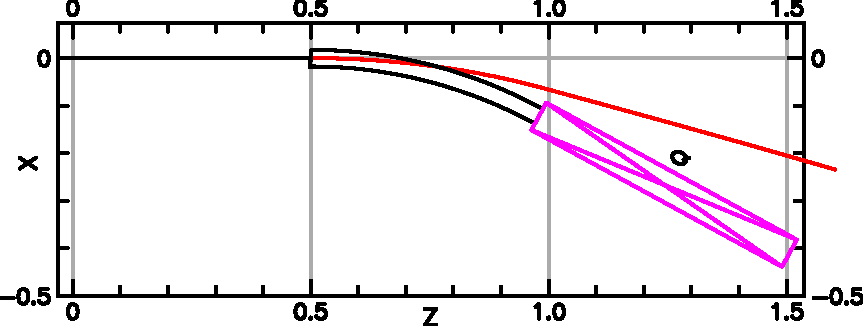
\includegraphics[width=0.6\textwidth]{plot-plan-orbit.pdf}
  \caption{The \vn{floor_plan} plot can display the particle orbit (orange line).}
  \label{f:floor.orbit}
\end{figure}

\begin{enumerate}[label=\thesection.\arabic{enumi}]
\item Try placing other plot templates onto the plot page, such as \vn{b_field}.
%
\item Use the \vn{set} command to set the \vn{draw_symbols} curve logical for the curves
in the \vn{beta} plot to True. What does the \vn{beta} plot look like now?
%
\item
The \vn{floor_plan} plot can include a drawing of the particle trajectory. As an example, do the
following:
\begin{enumerate}
\item
run \tao with the \vn{simple.bmad} lattice and use the \vn{place} command to display a
\vn{floor_plan} plot (\sref{s:disp.plot}).
\item
Set the following parameters of the graph of the \vn{floor_plan}:
\begin{code}
set graph floor floor_plan%orbit_scale = 100 
set graph floor_plan floor_plan%orbit_width = 8 
\end{code}
\item
You can now see the particle trajectory. Move this trajectory by varying the \vn{hkick} parameter of
element \vn{B}. For example:
\begin{code}
set ele b hkick = 0.003
\end{code}
You should see something like \fig{f:floor.orbit}. For more information (and more pretty pictures), 
see the \vn{Floor Plan Drawing} section (\extref{T-s:floor.plan}) of the \tao manual.
\end{enumerate}
%
\item
What is the command to scale the x-axis for all the plots with one command? Use this to scale the
x-axis for all plots to be the range [0.5, 1.5].
%
\end{enumerate}

\newpage

%------------------------------------------------------------------------------
%------------------------------------------------------------------------------
\Section{Model, Design and Base Lattices in Tao}
\label{s:three.lat}

When \tao runs, \tao instantiates three lattices
(Technically, \tao instantiates three lattices per \vn{universe}. See \sref{s:multi.uni}):
\begin{description}
\item[Design Lattice] \Newline
The \vn{design} lattice corresponds to the lattice read in from the lattice
description file(s). Parameters in this lattice are never varied.
\item[Model Lattice] \Newline
Initially, when \tao is started, The \vn{model} lattice is the same as the \vn{design}
lattice. Parameters in the \vn{model} lattice are allowed to vary. That is, all commands to vary
lattice parameters vary parameters of the \vn{model} lattice.
\item[Base Lattice] \Newline
The \vn{base} lattice is a reference lattice used so that changes in the \vn{Model} lattice may be
easily viewed. The \vn{Design} lattice can also be used as a reference lattice but since the
parameters of the \vn{design} lattice are fixed, this is not always desirable. The parameters of the
\vn{base} lattice are set by setting the parameters of the \vn{base} lattice equal to the present
state of the \vn{model} lattice.
\end{description}

\begin{figure}[tb]
  \centering
  \begin{subfigure}[t]{0.48\textwidth}
    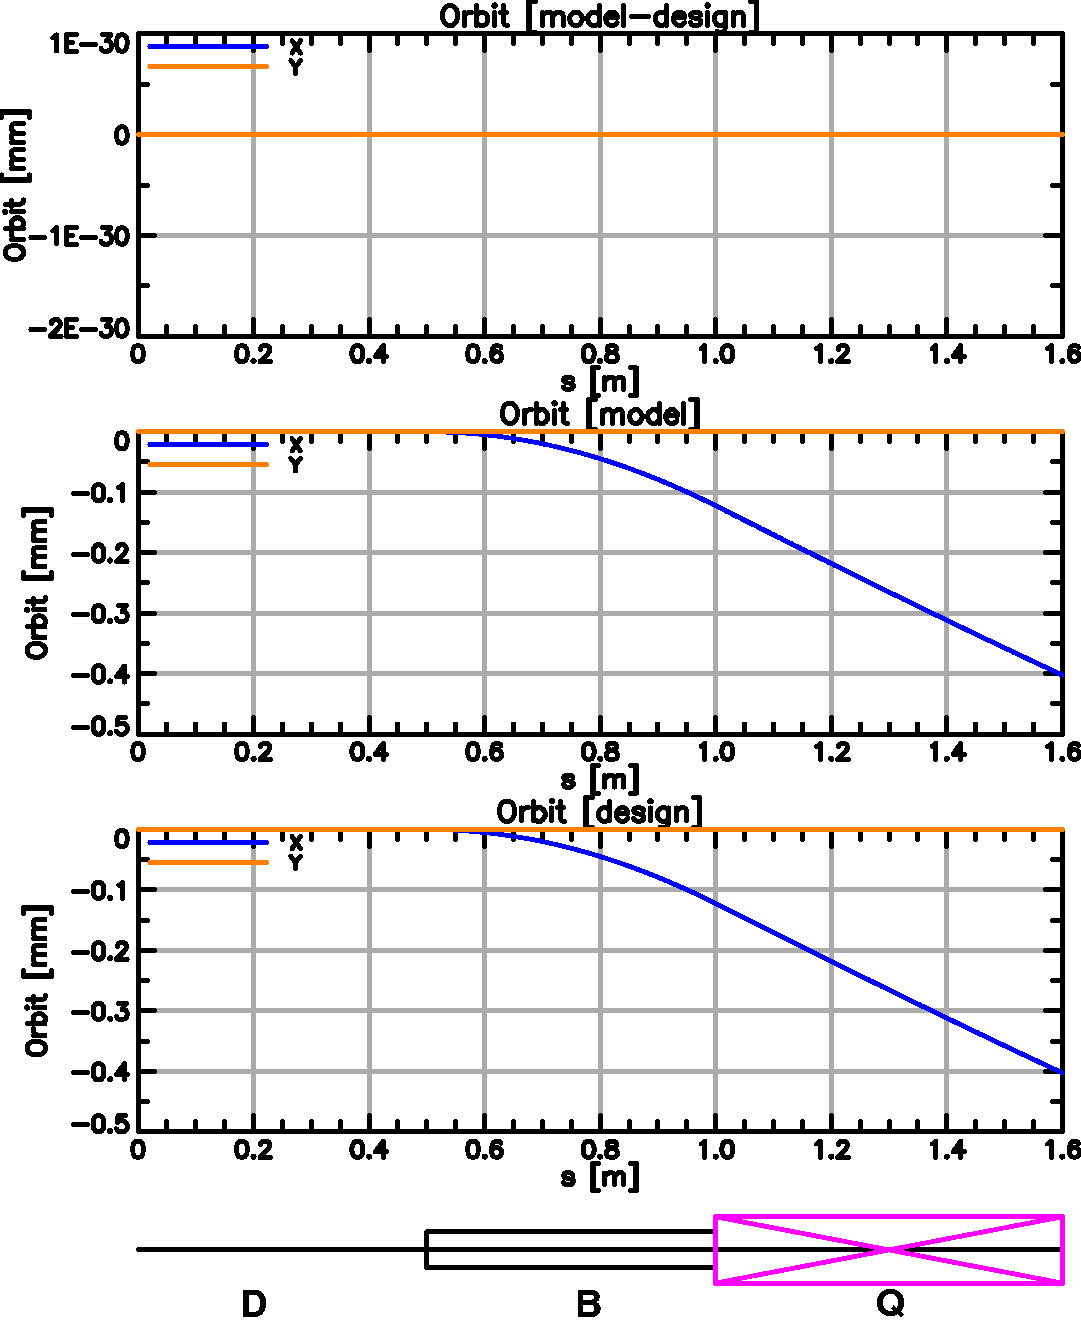
\includegraphics[width=\textwidth]{model-equal-design.pdf}
    \caption{Initially, the \vn{model} lattice and the \vn{design} lattices are the same.}
    \label{f:model.eq.design}
  \end{subfigure}
  \hfil
  \begin{subfigure}[t]{0.48\textwidth}
    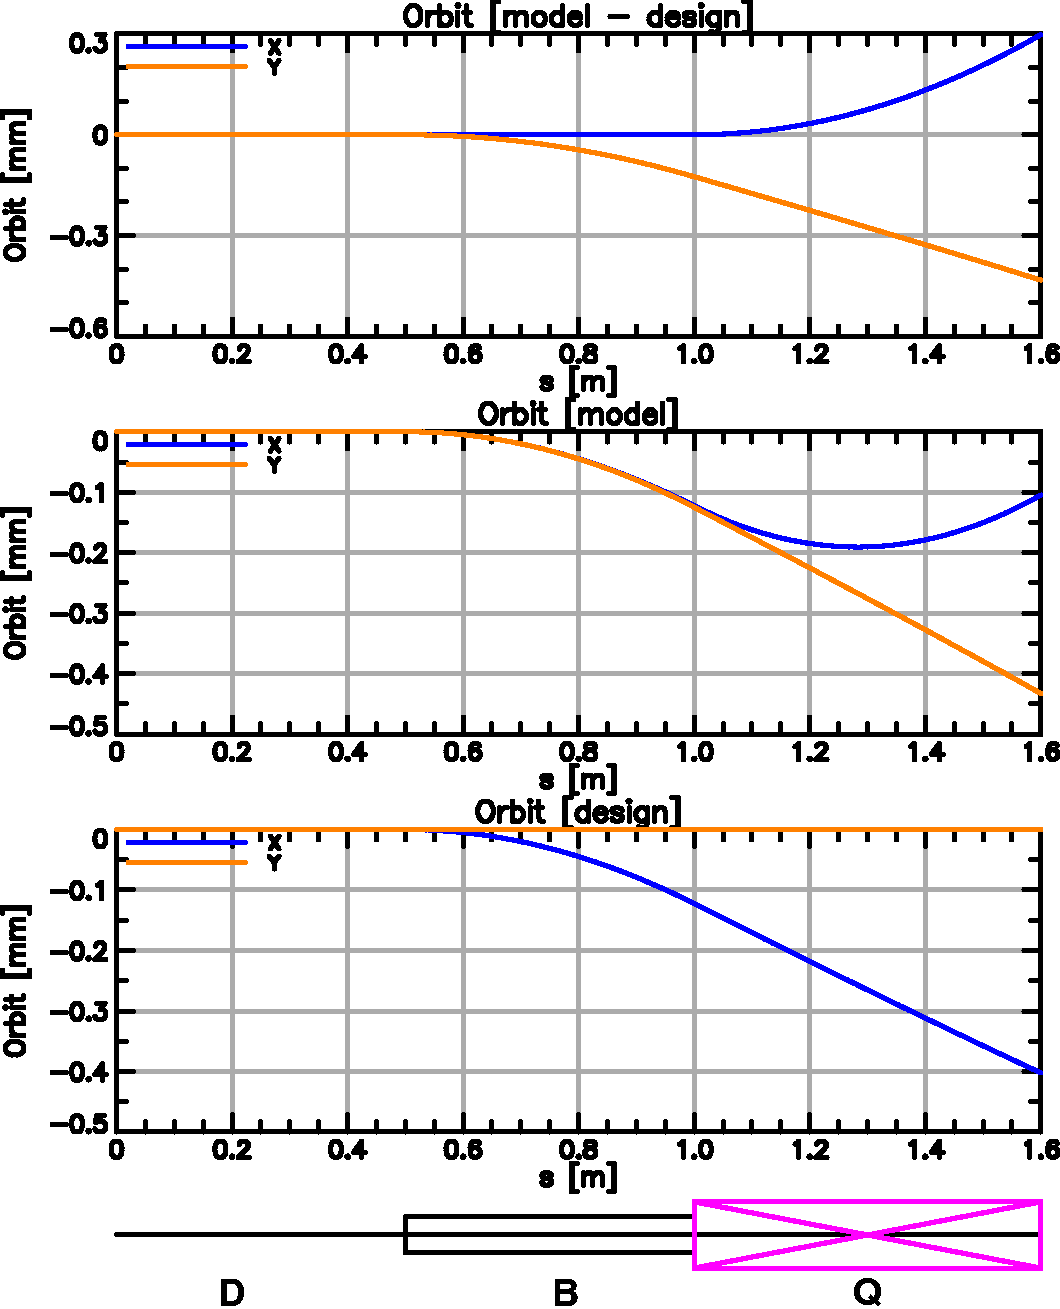
\includegraphics[width=\textwidth]{changed-model.pdf}
    \caption{The \vn{set} and \vn{change} commands will modify \vn{model} lattice parameters.}
    \label{f:changed.model}
  \end{subfigure}
  \caption{}
\end{figure}

%----------------------------------------------------------
\subsection{Changing Model Parameters}
\label{s:change}

To see the difference between the \vn{model} and \vn{design} lattices, start \tao as explained in
section~\sref{s:tao.run} with the lattice file \vn{simple.bmad}.

Now issue the following commands:
\begin{code}
Tao> place r23 orbit
Tao> place r13 orbit
Tao> set plot r33 component = design          ! Bottom plot
Tao> set plot r13 component = model - design  ! Plot difference orbit
Tao> scale
\end{code}
The ``\vn{set plot <plot_name> component = ...}'' command sets where the data to be plotted
comes from.  The result is shown in Figure~\ref{f:model.eq.design}. The bottom plot shows the
\vn{design} lattice orbit, the middle plot shows the \vn{model} lattice orbit and the top plot shows
the difference in orbits between \vn{model} and \vn{design}. Since the two lattices are the same
when \tao is started, the difference orbit is zero.

Now change the \vn{model} lattice using the following commands:
\begin{code}
Tao> change element b vkick  -0.0005   ! Changes by a given delta
Tao> set element q hkick = 0.001       ! Another way of changing a parameter.
Tao> scale
\end{code}
The \vn{change} command changes real numbers by a given delta. The \vn{set} command sets a 
parameter to a specific value. Unlike the \vn{change} command, 
the \vn{set} command can also be used with integer, string and logical
parameters.  The result is shown in Figure~\ref{f:changed.model}. Since now
the \vn{model} lattice is not the same as the \vn{design} lattice, the difference orbit is non-zero.

\begin{figure}[tb]
  \centering
  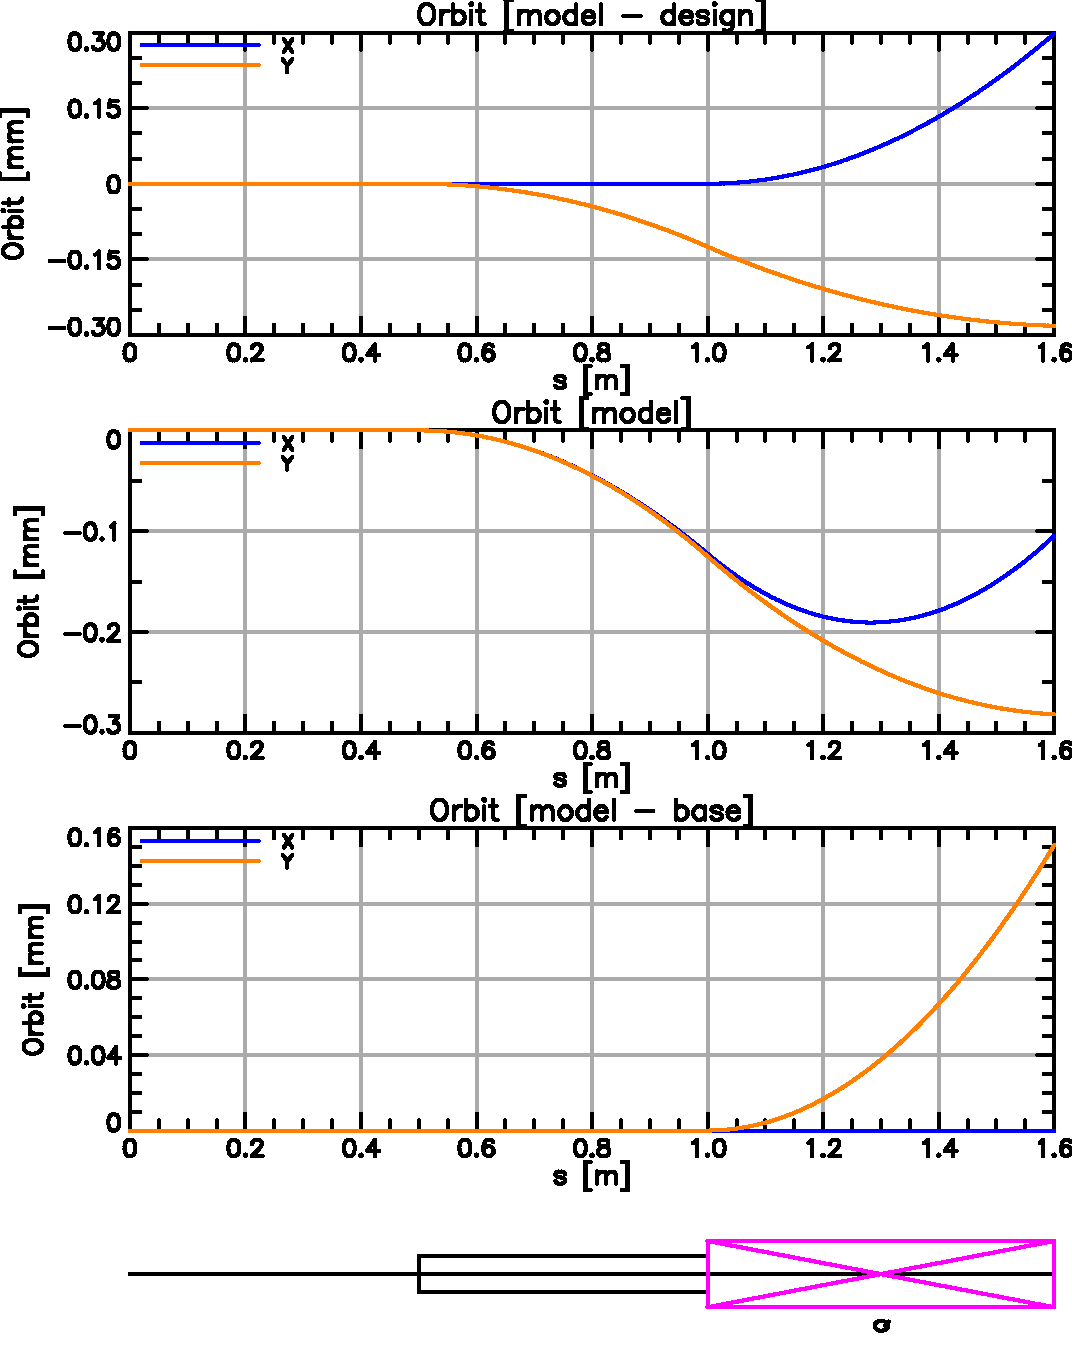
\includegraphics[width=0.6\textwidth]{with-base.pdf}
  \caption{The \vn{base} lattice is used to view changes when the reference lattice configuration
does not correspond to the \vn{design} lattice.}
  \label{f:base}
\end{figure}

%----------------------------------------------------------
\subsection{Using the Base Lattice}

The \vn{base} lattice is used to view changes when the desired reference lattice does not
correspond to the \vn{design} lattice.

Continuing from the previous section, issue the following commands:
\begin{code}
Tao> set lattice base = model  ! Set the Base lattice = Model lattice.
Tao> set plot r33 component = model - base
Tao> set ele q vkick = 5e-4
Tao> scale
\end{code} 
The \vn{set lattice} command sets the \vn{base} lattice equal to the \vn{model}
lattice. The third command varies the \vn{model} lattice.  The result is shown in
Figure~\ref{f:base}. The bottom plot of the orbit difference between \vn{model} and
\vn{base} is not the same as the orbit difference between \vn{model} and \vn{design}.

\vspace{1in}

%----------------- 
\subsection{Exercises [Answers in Section \sref{s:ans.model}]}
\label{s:three.lat.ex}

\begin{enumerate}[label=\thesection.\arabic{enumi}]
\item
Modify the middle graph in Fig.~\ref{f:base} so that the vertical orbit curve becomes the horizontal
orbit of the \vn{design} lattice.
\item
To save on typing, alias commands may be defined. Define an alias command called \vn{setit} so that
typing ``\vn{setit 1e-6}'' is equivalent to ``\vn{set ele q vkick = 1e-6}''. Hint: Look in the
manual or type ``\vn{help alias}'' to get more information on setting and using alias commands.
Note: Do not confuse \tao alias commands with the alias string component of a lattice element.
\end{enumerate}

\newpage

%------------------------------------------------------------------------------
%------------------------------------------------------------------------------
\Section{Optimization with Tao}
\label{s:optimization}

%----------------------------------------------------------
\subsection{What is Optimization?}
\label{s:opt.what}

``Optimization'' is the process of varying (model) lattice parameters to create a lattice with a
certain set of properties as close to a ``desired'' state as possible. Optimization is covered in
detail in the ``Optimization: Lattice Correction and Design'' chapter in the \tao manual.

Optimization problems generally fall into one of two categories. One category involves ``lattice
design'' where lattice parameters are varied to achieve some set of ideal properties. For example,
varying sextupole magnet strengths in order to give maximum dynamic aperture.

The other category of optimization problems involves ``lattice correction''. Problems in this
category involve matching the \vn{model} lattice to actual measured data.  For example, orbit
flattening involves varying steering in the \vn{model} lattice so that the orbit calculated from the
\vn{model} lattice matches as close as possible the measured orbit. The steering strengths in the
\vn{model} lattice can then be used to calculate what changes are needed to correct the orbit
as discussed section~\sref{s:cor.orbit}. 

An example of lattice design is given below. An example of lattice correction is given in
Chapter~\sref{s:opt.cor}.

%----------------------------------------------------------
\subsection{Optimization Overview and the Merit Function}
\label{s:opt.overview}

Optimization involves ``\vn{data}'' and ``\vn{variables}''. \vn{Data} are the parameters to be
optimized.  For example, orbit positions when flattening an orbit or the value of beta at the
interaction point when designing a lattice. \vn{Variables} are what is to be varied which can be
steering strengths, magnet positions, etc. 

Each datum has a set of associated parameters. For example, each datum has ``\vn{model}'' and
``\vn{design}'' values which is the value of the datum as calculated from the \vn{model} and
\vn{design} lattices. Each datum also has a ``\vn{measured}'' value which is set by the User. This
value can be from an actual measurement which is typical when doing lattice correction or may be the
desired value of the datum which is typical when doing lattice design. This is further discussed in
section \sref{s:data}. 

Like datums, each variable has a number of associated parameters. For example, each variable has a
``\vn{model}'' value which controls the corresponding value or values (a variable can control
multiple parameters simultaneously) in the \vn{model} lattice. There are also ``\vn{low_lim}'' and
``\vn{high_lim}'' values that can be set by the user that are used to keep the variable \vn{model}
value within a given range. This is further discussed in section \sref{s:var}.

Optimization involves minimizing one or more ``objectives'' or ``merit functions''. \tao itself
implements ``single objective'' optimization. For ``multiple objective'' optimization, there is a
separate program called \vn{moga} that can be used (\sref{s:programs}). The general form of the
merit function \vn{M} in \tao is
\begin{equation}
  {\cal M} \equiv 
    \sum_{i} w_i \, \bigl[ \delta D_i \bigr]^2 + 
    \sum_{j} w_j \, \bigl[ \delta V_j \bigr]^2
  \label{m1}
\end{equation}
where the first sum is a sum over the \vn{data} and the second sum is a sum over the
\vn{variables}. The $w_i$ and $w_j$ are weights specified by the user and the $\delta D_i$ and
$\delta V_j$ are functions of the data and variables. The merit function is discussed in depth in
Chapter~\extref{T-c:opti} in the \tao manual.

The form of the $\delta D_i$ can be different for each datum and similarly the form of $\delta V_j$
can be different for each variable and will be illustrated below in the example optimization.

There are several different optimizers that can be used with \tao. The one optimizer that is good
for finding global merit function minima is the \vn{de} (differential evolution) optimizer. All of
the others are good for finding local minima.

%----------------------------------------------------------
\subsection{Lattice Design Example: Initialization}
\label{s:opt.files}

An example of lattice design is given in the following section. For a lattice correction example, see 
chapter~\sref{s:opt.cor}.

The files used to illustrate lattice design optimization are in the directory 
\begin{code}
bmad-doc/tutorial_bmad_tao/lattice_files/lattice_optimization
\end{code}
Copy these files to your working directory. Here the main initialization file is named
\vn{tao.init}. Since this is the default name for initialization files (\sref{s:init.file}), and
since the \vn{tao.init} file contains the name of the lattice file, \tao can be started without the
\vn{-lat} option (\sref{s:tao.run}).

There are four files here:
\begin{lstlisting}[mathescape]
$\textbf{lat.bmad}$               ! Lattice file.
$\textbf{tao.init}$               ! Primary Tao initialization file. Includes plotting setup.
$\textbf{setup.tao}$               ! Command file run at startup.
$\textbf{optimized_var.out}$         ! Output optimized values
\end{lstlisting}

The file \vn{tao.init} is the main initialization file (\sref{s:init.file}). The file is divided
into three parts. The first part sets some general parameters while the next two sections setup data
\sref{s:data} and variable \sref{s:var} lists.
\begin{code}
&tao_start
  startup_file = "setup.tao"
/

&tao_design_lattice
  n_universes = 1
  design_lattice(1)%file = "lat.bmad"
/

&tao_plot_page
  plot_page%size = 500, 400
  place(1) = "layout", "lat_layout"
  place(2) = "r12", "beta"
  place(3) = "r22", "key"
/
\end{code}
Namelist format is used as explained in Section~\sref{s:init.file}. A single \vn{universe} will be
used (\sref{s:multi.uni}) and the lattice file name for the universe is ``\vn{lat.bmad}''. The
command file ``\vn{setup.tao}'' will be run after all other initialization is complete.

The \vn{tao_plot_page} namelist sets some plotting parameters. The setting of \vn{plot_page%size}
overrides the default size of the plot window and the \vn{place(1)}, \vn{place(2)}, and \vn{place(3)}
settings define initial placement of plots (\sref{s:disp.plot}).

The startup command file \vn{setup.tao} defines an \vn{alias} commands:
\begin{code}
alias opt run lm
\end{code}
This defines the command ``\vn{opt}'' to be equivalent to ``\vn{run lm}''. The \vn{run} command
starts optimization and the ``\vn{lm}'' option specifies the Levenburg-Marquardt optimizer which is
a good optimizer for finding a local minimum. See the \vn{Tao Commands} chapter in the \tao manual
for more details.

%----------------------------------------------------------
\subsection{Data in Tao}
\label{s:data}

In order to optimize, you must tell Tao what \vn{data} will contribute to the merit function. A
detailed description on how to do this is given in the ``\vn{Data}'' chapter of the \tao manual.

The data that is used in the present example is defined in the middle section of the \vn{tao.init}
file:
\begin{code}
&tao_d2_data
  d2_data%name = "twiss"
  n_d1_data = 2
/

&tao_d1_data
  ix_d1_data = 1
  d1_data%name = "a"
  datum(1) =  "beta.a"     "" "" "END"   "target"  12.0   1e1
  datum(2) =  "alpha.a"    "" "" "END"   "target" -0.4    1e2
/

&tao_d1_data
  ix_d1_data = 2
  d1_data%name = "b"
  datum(1) =  "beta.b"     "" "" "END"   "target"  12.0   1e1
  datum(2) =  "alpha.b"    "" "" "END"   "target" -0.4    1e2
/
\end{code}


\begin{figure}[b]
  \centering
  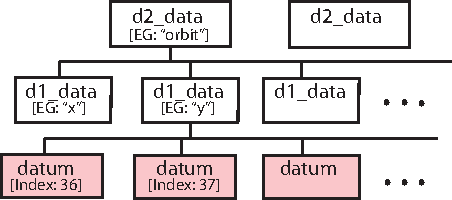
\includegraphics[width=0.90\textwidth]{data-tree.pdf}
  \caption{
Data is grouped into a three level tree. A \vn{d2_data} structure holds a set of \vn{d1_data}
structures. A \vn{d1_data} structure holds an array of \vn{datums}.}
  \label{f:data.tree}
\end{figure}

In general, the \vn{data} is grouped into a three level tree as illustrated in
Figure~\ref{f:data.tree}. Nodes at the the highest level are instances of what is called
\vn{d2_data} structures. For example, a \vn{d2_data} structure may be setup to hold \vn{orbit} data.
In the present case, there is a single \vn{d2_data} structure named ``\vn{twiss}''. 

A \vn{d2_data} structure will hold an array of one or more \vn{d1_data} structures. For example, a
\vn{orbit} \vn{d2_data} structure may hold ``\vn{x}'' and \vn{y}'' \vn{d1_data} structures which
represent horizontal and vertical orbit data. In the present case, the \vn{twiss} \vn{d2_data}
structure has two \vn{d1_data_structures} named ``\vn{a}'' and ``\vn{b}'' representing the two
transverse normal modes of oscillation. The syntax to refer to a particular \vn{d1_data} structure
is:
\begin{code}
  d2-data-name.d1-data-name
\end{code}
So with the above example, the \vn{a} structure would be referred to as \vn{twiss.a} .

A \vn{d1_data} structure will hold an array of one or more \vn{datum} structures. For example, the
\vn{x} \vn{d1_data} structure contained in an \vn{orbit} \vn{d2_data} structure may be setup with an
array of datums, one for each beam position monitor in the machine, with each datum representing a
horizontal orbit measurement at a specified BPM. In this case, both \vn{a} and \vn{b} \vn{d1_data}
structures hold two datums, one representing {\textbeta} and {\textalpha} Twiss values.  To refer to
an individual \vn{datum} use the syntax:
\begin{code}
  d2-data-name.d1-data-name[datum-index]
\end{code}
where \vn{datum-index} is the index for the datum. So with the above example, the first datum in
\vn{twiss.a}, which is the \vn{a}-mode {\textbeta}, would be referred to as \vn{twiss.a[1]} .

An individual \vn{datum} is structure that has a number of components. With the present
\vn{tao.init} file, seven components of each datum are set. These components are, in order:
\begin{code}
data_type       ! Type of data: "orbit.x", etc.
ele_ref_name    ! Name of reference lattice element
ele_start_name  ! Name of starting lattice element when there is a range
ele_name        ! Name of the lattice element where datum is evaluated.
merit_type      ! Type of constraint: "target", "max", "min", etc.
meas            ! Measured datum value.
weight          ! Weight for the merit function term
\end{code}
Thus for the \vn{twiss.b[2]} datum which is set on the line:
\begin{code}
  datum(2) =  "alpha.b"    "" "" "END"   "target" -0.4    1e2
\end{code}
The \vn{data_type} component is set to ``\vn{alpha.b}'' [For a list of data types that \tao
recognizes, see the \vn{Tao Data Types} section (\extref{T-s:data.types}) of the \vn{Data} chapter
of the \tao manual.], the \vn{ele_ref_name} and \vn{ele_start_name} are set to the blank
string. These parameters are not used in the present example.

The \vn{ele_name} component for \vn{twiss.b[2]} is set to ``\vn{END}'' which is where the datum is
to be evaluated. Since the \vn{merit_type} is set to \vn{target}, this means that $\delta D$ in
\Eq{m1} is evaluated using the equation
\begin{lstlisting}[mathescape]
$\delta D$ = model - meas
\end{lstlisting}
where \vn{model} is the value as calculated from the \vn{model} lattice and \vn{meas} is the
``\vn{measured}'' value as set on the datum line. For \vn{twiss.b[2]}, \vn{meas} is set to -0.4.
Also the weight $w$ for \vn{twiss.b[2]} is set to 100.  Thus if the model b-mode alpha function is, say,
1.0 at element \vn{END}, then this datum would contribute $100*(1.0 - 0.4)^2$ to the merit function.

Start \tao (remember, no \vn{-lat} argument needed). The \vn{d2_data} structures can be shown with
the command \vn{show data}:
\begin{code}
Tao> show data

  Name                                 Using for Optimization
  twiss.a[1:2]                                   Using: 1:2
  twiss.b[1:2]                                   Using: 1:2
\end{code}

To see a list of datums for an individual \vn{d1_data} structure append the \vn{d1_data} name after \vn{show data}.
For example:
\begin{code}
Tao> show data twiss.b
Data name: twiss.b
                    ...                                           |   Useit
                    ...  Ele         Meas       Model      Design | Opt  Plot
1  beta.b <target>  ...  END    1.200E+01   9.292E+00   9.292E+00     T     F
2  alpha.b <target> ...  END   -4.000E-01  -4.427E-01  -4.427E-01     T     F
                    ...  Ele         Meas       Model      Design | Opt  Plot
                    ...                                           |   Useit
\end{code}

To see the parameters of an individual datum append the datum name after \vn{show data}.
For example:
\begin{code}
Tao> show data twiss.a[2]

%ele_name          = END
... etc...
%data_type         = alpha.a
... etc...
%model             =  -4.42701763E-01
%design            =  -4.42701763E-01
... etc...
%good_model        = T
%good_design       = T
%good_base         = T
%good_meas         = T
%good_ref          = F
%good_user         = T
%good_opt          = T
%good_plot         = F
%useit_plot        = F
%useit_opt         = T
\end{code}
The \vn{useit_opt} logical indicates whether the datum will be used when the merit function is
evaluated. For example, if the \vn{meas} value has not been set, \tao will set \vn{good_meas} to
False and this will cause \tao to set \vn{useit_opt} to False. The user also as control as to whether
a datum will be used in optimization and this is controlled by setting the \vn{good_user} component.
The commands that control this are \vn{use}, \vn{veto} and \vn{restore}. Example:
\begin{code}
Tao> veto data twiss.a
  twiss.a[1:2]                                   Using:
  twiss.b[1:2]                                   Using: 1:2
\end{code}
In this example the two \vn{twiss.a} datums have been vetoed. It can be checked that the \vn{twiss.a} datums
now have their \vn{good_user} components set to False.

Notice that it does not matter to the optimization process how data is divided into \vn{d1_data} and
\vn{d2_data} groups. It is only a matter of convenience to the user. Also a given \vn{d1_data} group
of data does not have to contain data of a single type. Thus the \vn{twiss.a} datums include both
\vn{beta} and \vn{alpha} type data.

%----------------------------------------------------------
\subsection{Variables in Tao}
\label{s:var}

In order to optimize, you must tell Tao what \vn{variables} you want to vary to minimize the merit
function. A detailed description on how to construct \vn{variables} is given in the ``Variables''
chapter of the \tao manual.

The variables that are used in the present example are defined in the bottom section of the
\vn{tao.init} file:
\begin{code}
&tao_var
  v1_var%name = "quad"
  search_for_lat_eles = "Quad::*"
  default_step = 1e-4
  default_attribute = "k1"
  default_merit_type = "limit"
  default_low_lim = -50
  default_high_lim = 50
  default_weight = 1
  ix_min_var = 1
  default_key_delta = 1e-2
  default_key_bound = T
/
\end{code}
Just like \vn{data}, \vn{variables} are grouped into a two level tree as illustrated in
Fig.~\ref{f:var.tree}.  The top level nodes of the tree are called \vn{v1_var} structures. In this
example a \vn{v1_var} structure is defined called \vn{quad} which controls the \vn{k1} attribute of
all element whose name matches \vn{quad::*}. This will match to all quadrupoles. In this case, the
lattice has 6 quadrupoles named \vn{Q1} through \vn{Q6}. Thus there will be an array of 6
\vn{variables} associated with the \vn{quad} \vn{v1_var} structure.

%----------------------------------------------------------

\begin{figure}[tb]
  \centering
  \includegraphics[width=0.90\textwidth]{var-tree.pdf}
  \caption{
Variables are grouped into a two level tree. A \vn{v1_var} structure holds an array of
\vn{variables}. Illustrated is a \vn{var_var} structure holding an array of variables with each
variable controlling the \vn{hkick} attribute of a particular lattice element.}
  \label{f:var.tree}
\end{figure}

%----------------------------------------------------------

To refer to an individual variable use the syntax:
\begin{code}
v1-var-name[var-index]
\end{code}
where \vn{var-index} is the index of the variable. For example, the first variable in the \vn{quad}
structure is \vn{quad[1]}.

The parameters like \vn{default_step} in the above namelist establish a default value for the
\vn{step} attribute of each variable that is created for the \vn{quad} structure. The \vn{step}
attribute is used by \tao to calculate derivatives that are used by some of the optimizers.
Essentially, to calculate derivatives, \tao varies the variable by $\pm$\vn{step} and looks at the
changes in the \vn{data}. Like many attributes associated with \vn{optimization} it is important
that the \vn{step} attribute be set properly. To small a setting and round-off error can throw off
the derivative calculation. On the other hand, if the value of \vn{step} is too large,
nonlinearities can throw off the calculation.

The \vn{weight} of a variable sets the value of $w_j$ in \Eq{m1}. Since the \vn{merit_type} in this case
is \vn{limit}, the $\delta V$ used in the merit function is:
\begin{equation}
  \delta V = 
    \begin{cases}
    \mbox{model} - \mbox{high\_lim}  & \mbox{model} > \mbox{high\_lim} \\
    \mbox{model} - \mbox{low\_lim}   & \mbox{model} < \mbox{low\_lim} \\
    0                                & \mbox{Otherwise}
    \end{cases}
\end{equation}
That is, the contribution to the merit function will be zero if the value of the variable is between
\vn{low_lim} and \vn{high_lim} which in this case is -50 and 50.

Running \tao, the \vn{v1_var} structures can be shown with the command \vn{show variable}: 
\begin{code}
Tao> show var
       Name                                      Using for Optimization
    quad[1:6]                                    1:6
\end{code}

To see a list of individual variables of a given \vn{v1_var} structure, append the \vn{v1_var}
name to the \vn{show variable} command:
\begin{code}
Tao> sho var quad
Variable name:  quad

 Index  Controlled Attribs(s)    Meas         Model        Design  Useit_opt
     1  Q1[K1]               8.6924-311    0.0000E+00    0.0000E+00       F
     2  Q2[K1]               8.6924-311    0.0000E+00    0.0000E+00       F
     3  Q3[K1]               8.6924-311    0.0000E+00    0.0000E+00       F
     4  Q4[K1]               8.6924-311    0.0000E+00    0.0000E+00       F
     5  Q5[K1]               8.6924-311    0.0000E+00    0.0000E+00       F
     6  Q6[K1]               8.6924-311    0.0000E+00    0.0000E+00       F
 Index  Controlled Attribs(s)    Meas         Model        Design  Useit_opt
\end{code}

To see the parameters of an individual variable, append the variable name to the \vn{show var}
command. Example:
\begin{code}
Tao> sho var quad[2]
%ele_name         = Q2
%attrib_name      = K1
... etc...
%exists           = T
%good_var         = T
%good_user        = T
%good_opt         = T
%useit_opt        = T
... etc...
\end{code}
The \vn{useit_opt} logical indicates whether the variable will be used in the optimization process.
The user has some control as to whether a variable will be used in optimization and this is controlled
by setting the \vn{good_user} component. The commands that control this are \vn{use}, \vn{veto} and
\vn{restore}. Example:
\begin{code}
Tao> veto var quad[4]
  quad[1:6]                                      Using: 1:3 5:6
\end{code}

Variable properties can also be changed within Tao. For example, 
\begin{code}
Tao> set var quad[1:4]|low_lim = -1
\end{code}
will set the lower limit for the first four quads.

Notice that, like data, it does not matter to the optimization process how variables are divided
groups. It is only a matter of convenience to the user. Also a given \vn{v1_var} instance, the array
of associated \vn{variables} does not all have to be of a single type.

If you want to have one \tao \vn{variable} control a set of parameters, construct an \vn{overlay} or
\vn{group} element (\sref{s:control}) and then have the \tao variable control the overlay or
group. For example, the following overlay defined in the lattice file gangs the \vn{k1} parameters
of elements \vn{Q1} and \vn{Q3} together:
\begin{code}
ps1: overlay = {Q1, Q3}, var = {k1}, k1 = 0.8
\end{code}

\begin{figure}[b]
  \centering
  \includegraphics[width=5in]{keyboard.pdf}
  \caption
{Ten pairs of keys on the keyboard are bound to ten variables so that pressing a key of a given pair
will either increment or decrement the associated variable. The first key pair bound to variable
number 1 are the \vn{1} and \vn{Q} keys, etc.}
  \label{f:keyboard}
\end{figure}

%----------------------------------------------------------
\subsection{Key Bindings}
\label{s:key.bound}

Tao has two modes for entering commands. In \vn{single mode}, each keystroke represents a command.
That is, with a few exceptions, the user does not have to press the carriage control key to signal
the end of a command. This is to be contrasted with \vn{line mode}, which you have been using up to
now, where \tao waits until the return key is depressed to execute a command. \vn{single mode} is
useful for quickly varying parameters to see how they affect a lattice but the number of commands in
single mode is limited. \vn{Single mode} is covered in detail in the ``Single Mode'' chapter in the
\tao manual.

The main purpose of \vn{single mode} is to associate certain keyboard keys with certain variables so that
the pressing of these keys will change their associated model value of the variable. This is called
a \vn{key binding} and is illustrated in Figure~\ref{f:keyboard}.

\begin{figure}
  \centering
  \begin{subfigure}[t]{0.48\textwidth}
    \includegraphics[width=\textwidth]{opt0.pdf}
    \caption{Initial plot window showing the initial beta functions.}
    \label{f:opt0}
  \end{subfigure}
  \hfil
  \begin{subfigure}[t]{0.48\textwidth}
    \includegraphics[width=\textwidth]{opt1.pdf}
    \caption{Plot window after optimization showing the optimized beta functions.}
    \label{f:opt1}
  \end{subfigure}
  \caption{}
\end{figure}

Start \tao using the example optimization files (\sref{s:opt.files}) or use the \vn{reinit tao}
command to reinitialize \tao. The plot window should look like Figure~\ref{f:opt0}. The
\vn{key_table} plot in the middle shows what variables (\sref{s:var}) have been bound to what
keyboard keys. In this instance the \vn{quad[1]} variable is bound so that pressing the ``1'' key
will change \vn{quad[1]} by +\vn{delta}, and pressing the ``q'' key will change \vn{quad[1]} by
-\vn{delta}.  Pressing the shift key when pressing the ``1'' or ``q'' keys will change \vn{quad[1]}
by \vn{+10}$\times$\vn{delta} and \vn{-10}$\times$\vn{delta} respectively. Similarly, the \vn{quad[2]}
variable is bound to the \vn{2} and \vn{w} keys, etc.

Single mode and key bindings are useful for getting a feel for how variables affect the lattice. Get
into single mode by issuing the \vn{single_mode} command. Play around with varying variables. To
get out of single mode press capital \vn{Z}.

\newpage

%----------------------------------------------------------
\subsection{Running an optimization}
\label{s:opt.run}

Start \tao using the example optimization files (\sref{s:opt.files}) or use the \vn{reinit tao}
command to reinitialize \tao. The plot window should look like Figure~\ref{f:opt0}. 

To see what data and what variables are being used in the optimization, use the \vn{show data} and
\vn{show variables} commands as illustrated above or use the \vn{show optimizer} command:
\begin{code}
Tao> show opti
Data Used:
  twiss.a[1:2]                                   Using: 1:2
  twiss.b[1:2]                                   Using: 1:2
Variables Used:
  quad[1:6]                                      Using: 1:6

optimizer:        lm
Global optimization parameters (use "set global" to change):
  %de_lm_step_ratio              =   1.00000000E+00
  %de_var_to_population_factor   =   5.00000000E+00
  %lm_opt_deriv_reinit           =  -1.00000000E+00
  %lmdif_eps                     =   9.99999996E-13
  %merit_stop_value              =  -1.00000000E+00
  %svd_cutoff                    =   9.99999975E-06
... etc...
\end{code}
There are many parameters associated with optimization and it is important to carefully consider
what values these parameters have in order to be able to have a successful optimization.

To see what the biggest contributions to the merit function
are use the \vn{show top10} command:
\begin{code}
Tao> show top

Constraints                   ...   Ele/S     Target      Value      Merit  
twiss.b[1]  beta.b <target>   ...   END       1.200E+01   1.513E+01  9.82E+01
twiss.a[1]  beta.a <target>   ...   END       1.200E+01   9.292E+00  7.33E+01
twiss.b[2]  alpha.b <target>  ...   END      -4.000E-01  -2.527E-01  2.17E+00
twiss.a[2]  alpha.a <target>  ...   END      -4.000E-01  -4.427E-01  1.82E-01
quad[6]     Q6[K1]            ...   3.80     -5.000E+01  -1.000E+00  0.00E+00
quad[5]     Q5[K1]            ...   3.30      5.000E+01   1.000E+00  0.00E+00
... etc...

 figure of merit: 1.738388E+02

List of non-zero contributors to the Merit Function:
Name                           Merit           Sigma [= sqrt(Chi^2/N)]
twiss.b                        1.0034E+02      2.2179E+00
twiss.a                        7.3499E+01      1.9149E+00
\end{code}
This shows, among other things, that the value of the merit function is 173.8 and that the largest
contributor to the merit function is \vn{twiss.b[1]} which has a contribution of 98.2 which is over
50\%.

To run, say, the \vn{lm} optimizer use the \vn{run lm} command. In this case, this command
has been aliased to the \vn{opt} command by the \vn{setup.tao} command file that was run
at initialization (\sref{s:opt.files}):
\begin{code}
Tao> opt
Optimizing with: lm
Type ``.'' to stop the optimizer before it's finished.
[INFO] tao_dmodel_dvar_calc:
    Remaking dModel_dVar derivative matrix.
    This may take a while...

  Cycle      Merit   A_lambda
    1    5.4532E-01  1.00E-04
    2    8.7067E-02  1.00E-05
... etc...
   19    3.5034E-04  1.00E-22
   20    2.9333E-04  1.00E-23
Written: var1.out
   21    2.9333E-04  0.00E+00
\end{code}
The optimization has managed to reduce the merit function from to 2.9E-4 or about six orders of
magnitude. Further reductions in the merit function can be had by running the optimizer
repeatedly. At the end of optimization, \tao creates a file \vn{var1.out} which contains the
optimized variable values:
\begin{code}
 Q1[K1] =   7.76217267682967E-01
 Q2[K1] =  -1.40330956873957E+00
 Q3[K1] =   8.78773428675319E-01
 Q4[K1] =  -1.07943627873167E+00
 Q5[K1] =   1.29072113653010E+00
 Q6[K1] =  -4.57469896955973E-01
... etc...
\end{code}
This file should be virtually identical to the \vn{optimized_var.out} file (\sref{s:opt.files}). The
format of this file conforms to \bmad lattice file syntax so this file can be used to create a
lattice with the optimized values. One way to form a lattice with optimized values is to create a
new lattice file that calls the original lattice and \vn{var1.out}. That is, the new file would look
like:
\begin{code}
call, file = lat.bmad
call, file = var1.out
\end{code}

To print in Bmad format the variable values used in the optimization use the command:
\begin{code}
show var -bmad -good
\end{code}
To save directly to a file, add the write option:
\begin{code}
show -write solution.bmad var -bmad -good
\end{code}

\newpage

%----------------- 
%%\subsection{Exercises [Answers in Section \sref{s:ans.opt}]}
\subsection{Exercises}
\label{s:opt.ex}

\begin{figure}[tb]
  \centering
  \includegraphics[width=0.8\textwidth]{building-wall.pdf}
  \caption{
Optimization to keep a machine within existing building walls. A) Initial setup. The end of the machine (a
1~meter long dipole) is outside the walls (red and green semi circles). B) After optimization the machine is
safely inside the walls.}
  \label{f:b.wall}
\end{figure}

\begin{enumerate}[label=\thesection.\arabic{enumi}]
%------------------------
\item
\label{s:opt.ex1}
Start with the files in \vn{bmad-doc/tutorial_bmad_tao/lattice_files/lattice_optimization}. Change
all the quadrupole strengths to zero in \vn{lat.bmad} and change the alpha Twiss \vn{meas} targets
to -1. Now run with the \vn{opt} command and verify that the optimizer does not not find a good
solution! Why is this? The problem is that the good solutions (and there is more than one) are
outside of the local minimum that the optimizer is stuck in. 
Note: To easily reset the lattice use the command:
\begin{code}
set lattice model = design
\end{code}
%
\item
Start with the situation in Exercise~\ref{s:opt.ex1} and find a good solution by first using
\vn{single mode} to vary the quadrupole strengths to find an approximate solution. Then run the
\vn{lm} optimizer to polish the results. This is a general strategy, often there is no single method
that will work so a combination of methods is what is needed.
%
\item
Start with the situation in Exercise~\ref{s:opt.ex1} and find a good solution by first using the
\vn{de} optimizer which can find global minimums. Then run the \vn{lm} optimizer to polish the
results. Warning: Success here depends upon finding the right \vn{de} parameter settings to
use. This will take some thought and experimentation so successful completion of this exercise will
not be quick.
%
\item
This exercise shows how to do an optimization with a constraint that the machine stay within
existing building walls. If you get stuck, a working example can be viewed in the
directory:
\begin{code}
bmad-doc/tutorial_bmad_tao/lattice_files/building_wall_optimization
\end{code}

\begin{enumerate}
\item
Construct a lattice with a single element which is a 1~meter long bend with zero bend angle.
\item
Setup a \tao input file that defines two building wall sections as shown in
Figure~\ref{f:b.wall}A. The sections are two circular arcs of radius 0.8~meters and 1.2~meters.
\item
Setup two datums: \vn{wall[1]} and \vn{wall[2]}. The first datum constrains the end of the lattice
to be to the inside of the outside (left) wall with a 0.1~meter clearance. The second datum constrains
the end of the lattice to be to the outside of the inside (right) wall with a 0.1~meter clearance.
\item
Setup a variable to vary either the \vn{g} or \vn{angle} component of the bend.
\item
Run the \vn{lm} optimizer to produce Figure~\ref{f:b.wall}B. Voila! The machine is within the walls with
the desired clearance.
\item
When you startup \tao and the dipole is unbent, you should get an error message that looks something like:
\begin{code}
[ERROR | 2025-JUL-04 01:24:26] tao_set_invalid:
    No wall section found in the transverse plane of the evaluation point.
    FOR DATUM: wall[2] with data_type: wall.right_side
\end{code}
Explain why you are getting this message. Also explain why this message goes away when the dipole
gets bent enough. [Hint: Read carefully the description of how the datum value is computed.] Note
that not being initially able to compute a model value does not hinder the optimization.
\end{enumerate}

\end{enumerate}

\newpage

%------------------------------------------------------------------------------
%------------------------------------------------------------------------------
\Section{Lattice Correction (Including Orbit Correction)}
\label{s:opt.cor}

The previous chapter (\sref{s:opt.what}) discussed optimization and, in particular, how optimization
could be used for ``lattice design'' type problems. This chapter discusses ``lattice correction''
type optimization. In particular, this chapter shows how to calculate corrections to correct the
Twiss parameters using measured orbits. It is assumed that the reader is familiar with the material
in the previous chapter.

Side note: With an actual machine, calculating corrections is only one step in the correction
process. Also needed is the ability to take data and the ability to load corrections. The object
oriented nature of \tao's design makes it relatively straightforward to implement machine
communication within \tao itself. This allows \tao to act as an ``online model'' for the machine
control system. Programming with \bmad and \tao is outside of the scope of this tutorial and the
reader is referred to the appropriate sections of the \bmad and \tao manuals.

%------------------------------------------------------------------------------
\subsection{Correcting the Orbit}
\label{s:cor.orbit}

Before discussing Twiss parameter correction, consider the simpler case of correcting the orbit. The
\vn{design} lattice will represent the state we want the machine to be in. Typically, the orbit in
the \vn{design} lattice will be zero but that is not a necessary condition. The analysis starts
with an orbit measurement. By varying steerings in the \vn{model} lattice, the orbit, as calculated
in the \vn{model}, can be fit to the measured orbit.\footnote
  {
Typically, the measured orbit in a machine with a closed geometry (EG storage ring) will be the
closed orbit while the orbit in an open geometry machine (EG Linac) will be the orbit as measured
with the beam starting from some initial position. In the open geometry case, varying the initial
position in the model lattice along with steerings may be necessary to fit the orbit.
  }
If the fit is good, the orbit is corrected in
the machine by changing the actual steering strengths $K_{actual}$ by an amount $dK$ given by
\begin{equation}
  dK_{i} = K_{i}^{(design)} - K_{i}^{(model)}
  \label{dkkk}
\end{equation}
where $i$ denotes the $i$\th steering, and $K_{i}^{(design)}$ and $K_{i}^{(model)}$ are the
\vn{design} and \vn{model} values for the steering strengths respectively. Typically, the
\vn{design} steering strengths are zero but that is not necessary for the analysis.

\Eq{dkkk} is derived using the following logic: Once a fit to the measured data has been made, the
\vn{model} represents the actual state of the machine. On the other hand, the desired state is
represented by the \vn{design} lattice. Thus the difference $K_{i}^{(design)} - K_{i}^{(model)}$
represents ``desired - actual'' so the final state of the steering magnets after correction will be
\begin{code}
  Final_State = Initial_State + Change
              = Actual_State + (Desired_State - Actual_State)
              = Desired_State
\end{code}
There are a few points that should be kept in mind here. First, it does not matter to the
correction whether the deviations of the orbit from the ideal are caused by steering strength errors
or other errors such as dipole rolls or quadrupole offsets. To the extent that the measured orbit
can be well fit determines the extent to which the orbit can be corrected. For example, if an unwanted
kick is generated by some element at a spot that is far from any correctors, it will not be possible
to fit the measured orbit well and it will not be possible to make a good correction. If, on the
other hand, an unwanted kick is generated next to one corrector, the measured orbit can be well fit
and the \vn{model} lattice will have a strength change from the \vn{design} for that one
corrector. Varying that one corrector can then cancel out the unwanted kick.

Another point is that the correction algorithm will work with varying any set of parameters as long
as the variation in the parameters affect the \vn{model} data. Thus an analysis can be made using
dipole rolls and/or quadrupole offsets as variables or any combination thereof. If the fit is good,
rolling the dipoles and moving the quadrupoles will correct the orbit. With \tao, the User has
complete freedom to vary any parameters in the fitting process.

A third point is that the fitting process is independent of the strengths of the parameters in the
\vn{design} lattice. That is, the fit involves the actual machine state independent of what the
desired state is. It is not until the values needed for the correction are computed that the
parameter strengths in the \vn{design} lattice come into play. 

Typically, at the start of the fit, the \vn{model} lattice is, by default, equal to the \vn{design}
lattice but this is not necessary. Generally, the actual machine state is near enough to the
\vn{design} machine state so that the machine will behave roughly linearly with the variation in the
parameters (typically, if the machine parameters are far from the design values, it will not be
possible to store beam to take a measurement in the first place). This means that there will be only
one minimum merit function state so that the parameter values (steering strengths in this case) at
the end of the fit are independent of the starting state. To put this in other terms, the User
generally does not have to worry about the initial state of the \vn{model} at the start of a
fit. This is in contrast to the lattice design example in chapter~\sref{s:optimization}. With
lattice design, there are typically many local minima and it can take days of work to find a good
operating point. With lattice correction, on the other hand, the near linear nature of the problem
means that finding a solution in a machine with hundreds of correctors and hundreds of BPM readings
can be done in seconds.

%------------------------------------------------------------------------------
\subsection{Twiss Parameters Correction}
\label{s:twiss.cor}

As mentioned in the previous section, with \tao, the User has complete freedom to fit to any
arbitrary set of lattice parameters. \tao also gives the User complete freedom to optimize using any
arbitrary collection of data. In particular, as discussed below, by varying quadrupole strengths to
fit a multiple orbit data sets taken with multiple steering strength settings allows correction of
the Twiss parameters.

One way to correct Twiss parameters is to vary, one-by-one, the steerings in the machine and for
each varied steering, take before and after orbits. By fitting the measured orbit differences using
the \vn{model} quadrupole strengths, the strengths of the quadrupoles can be determined. With this,
the difference between the \vn{model} quadrupole strengths and the \vn{design} strengths gives the
needed quadrupole corrections. See \Eq{dkkk} where, in this case, the $K$'s represent quadrupole
strengths. In practice the steering strengths will also be included in the variable list. This
correction scheme is similar to the Orbit Response Matrix (ORM) approach in that both uses multiple
orbits to correct the Twiss parameters.

It should be mentioned that even without doing the correction step, the fitting of the data in 
itself gives values for the optics in the current state of the machine.

%------------------------------------------------------------------------------
\subsection{Twiss Parameter Correction Example Input Files}
\label{s:twiss.setup}

The example files used to illustrate correction of the Twiss parameters are in the directory 
\begin{code}
bmad-doc/tutorial_bmad_tao/lattice_files/twiss_correction
\end{code}
Copy these files to your working directory. There are six files:
\begin{lstlisting}[mathescape]
$\textbf{create_data.tao}$               ! For creating "measured" data. 
$\textbf{lat.bmad}$               ! Lattice file.
$\textbf{tao.init}$               ! Primary Tao initialization file.
$\textbf{tao_plot.init}$               ! Plot setup initialization file.
$\textbf{startup.tao}$               ! Command file run at startup.
$\textbf{set_meas.tao}$               ! Set measured data.
\end{lstlisting}

The lattice being used here has one horizontal steering named \vn{H1} and one vertical steering
named \vn{V2}. Two universes (\sref{s:multi.uni}) will be needed to store the measured
data. The first universe will hold the measured data from changing \vn{H1} and the second universe
will hold the measured data from changing from \vn{V2}.

The file \vn{tao.init} is the main initialization file (\sref{s:init.file}) and is similar to the
\vn{tao.init} file in Chapter~\sref{s:opt.files}. One difference is the the \vn{tao.init} file here
initializes \tao with two universes instead of one:
\begin{code}
&tao_design_lattice
  n_universes = 2
  design_lattice(1)%file = "lat.bmad"
  design_lattice(2)%file = "lat.bmad"
/
\end{code}
Here both universes use the same lattice.

The \vn{tao.init} file lists the secondary initialization files in the \vn{tao_start} namelist:
\begin{code}
&tao_start
  startup_file = "startup.tao"
  plot_file = "tao_plot.init"
/
\end{code}

%------------------------------------------------------------------------------
\subsection{Data Setup}
\label{s:twiss.data}

Data (\sref{s:data}) for the optimization is setup in the file \vn{tao.init} file. There is just one
\vn{d2_data} block called \vn{orbit}:
\begin{code}
&tao_d2_data
  d2_data%name = "orbit"
  universe = "*"
  n_d1_data = 2
  default_weight = 1e8
/

&tao_d1_data
  ix_d1_data = 1
  d1_data%name = "x"
  search_for_lat_eles = "det*"
/

&tao_d1_data
  ix_d1_data = 2
  d1_data%name = "y"
  search_for_lat_eles = "det*"
/
\end{code}
There are two \vn{d1_data} arrays for the horizontal and vertical orbits. A datum will be set up for
each element whose name begins with ``\vn{det}''. That is, at the four detectors in the lattice
\vn{det1} through \vn{det4}. The \vn{universe = *} setting results in an \vn{orbit} data block being
setup one for each universe.

%------------------------------------------------------------------------------
\subsection{Variable Setup}
\label{s:twiss.var}

The variables (\sref{s:var}) setup is in the file \vn{tao.init}. There are three \vn{v1_var}
blocks --- for quadrupole strengths and tilts, along with steering strengths. By varying quadrupole
tilts, the coupling can be corrected. [Typically, coupling --- that is, coupling between horizontal and
vertical orbits due to skew fields --- is corrected by adjusting the strength of skew quadrupoles. Here,
to simplify things somewhat, the same quadrupoles are used for both beta and coupling correction.]

The variable blocks are defined in \vn{tao_var} namelists The quadrupole strength block is
\begin{code}
&tao_var
  v1_var%name = "quad_k1"
  search_for_lat_eles = "Quad::*"
  default_step = 1e-4
  default_attribute = "k1"
  default_merit_type = "target"
  default_weight = 1
  ix_min_var = 1
  default_key_delta = 1e-2
  default_key_bound = T
/
\end{code}
The \vn{search_for_lat_eles} setting will searches for quadrupole elements in all universes. All
quadrupoles of a given name in all universes will be bound together with a single variable. In this
case there are two quadrupoles named \vn{q1} and \vn{q2} in each universe so the \vn{quad_k1}
variable array, which has the name \vn{quad_k1[1]}, will have two elements. One element will control
the \vn{k1} attribute of the \vn{q1} element in universe 1 and the the \vn{k1} attribute of the
\vn{q1} element in universe 2. Similarly the other variable, \vn{quad_k1[2]} will control the
\vn{k1} attribute of the \vn{q2} elements.

When a variable controls multiple elements, the controlled parameters (the \vn{k1s} of the two
\vn{q1} quads in this case) can have different values as long as the \vn{model} value of the
variable is not touched. When the \vn{model} value is set, either during the optimization or with a
\vn{set} or \vn{change} command, all the controlled parameters will be set to the same value as the
\vn{model} value of the variable.  This setup mirrors the orbit measurement conditions were the
quadrupole strengths were the same for all measurements.

The \vn{merit_type} is set to \vn{target} which means that the contribution to the merit function in \Eq{m1}
will be 
\begin{equation}
  \delta V = \mbox{model} - \mbox{measured}
\end{equation}
Here \vn{measured} is the value of the quadrupole strength as ``measured'' when the orbit was
obtained.  Typically, magnet strengths are ``measured'' using the known calibration between current
going through the field windings or, if it is a permanent magnet, the measured value is taken to be
the field that was measured on the bench before installation. 

The reason why the merit function is setup to have a contribution from the variables is to avoid
near-degeneracies where, if there where no $\delta V$ terms, inaccuracies in the orbit measurement
coupled with magnets that have a similar effect on the orbit results in the optimization minimum
being a state where the near-degenerate magnets have large unphysical strengths but the \vn{model}
orbit will look reasonable since the effect of the near-degenerate magnets nearly cancel one
another. The trick is to adjust the weights for the $\delta V$ terms to be large enough to keep the
magnet strengths reasonable but not too large that the fit of the orbit is degraded due to
inaccuracies in the variable measurement value.

The second variable block defines variables that control quadrupole tilts. These variables are setup
similar to the quadrupole strength variables.

The third variable block holding the steering strengths is setup with
\begin{code}
&tao_var
  v1_var%name = "steering"
  default_step = 1e-4
  default_merit_type = "target"
  default_weight = 1
  default_key_delta = 1e-2
  default_key_bound = T
  var(1:2)%universe  =  1,       2
  var(1:2)%ele_name  = "h1",    "v2"
  var(1:2)%attribute = "hkick", "vkick"
/
\end{code}
Here there are two variables \vn{steering[1]} and \vn{steering[2]}. \vn{steering[1]} controls the
\vn{hkick} attribute of element \vn{h1} in universe 1 and \vn{steering[2]} controls the
\vn{vkick} attribute of element \vn{v2} in universe 2.

%------------------------------------------------------------------------------
\subsection{Plotting Setup}
\label{s:twiss.plot}

For details of how to setup custom plots, see the \vn{Initializing Plotting}
(\extref{T-s:init.plot}) section of the \vn{Tao Initialization} chapter of the \tao manual.  Here
the plotting setup is done in the \vn{tao_plot.init} file. This file defines a plot template
(\sref{s:disp.plot}) called \vn{data_orbit} in a \vn{tao_template_plot} structure:
\begin{code}
&tao_template_plot
  plot%name = "data_orbit"  ! Name of template plot.
  plot%x_axis_type = "s"    ! Graph x-axes are longitudinal s-coordinate.
  plot%autoscale_gang_y = F ! So scale command scales the graphs separately.
  plot%n_graph = 2          ! There are 2 associated graphs.
/
\end{code}
This template plot has two associated graphs defined in two \vn{tao_template_graph} namelists below
the \vn{tao_template_plot} namelist. The first graph's namelist looks like:
\begin{code}
&tao_template_graph
  graph_index = 1               ! First graph.
  graph%name = "x"              ! Graph name is "data_orbit.x"
  graph%box = 1, 1, 1, 2        ! Graph is in lower half of the plot region.
  graph%title = "X Orbit [mm]"  ! Graph title
  graph%y%label = "X (mm)"      ! Graph y-axis label.
  ... etc. ...
\end{code}
This graph is named ``\vn{x}'' so the fully qualified name is ``\vn{data_orbit.x}''. There are
three curves associated with this graph and are defined further down in this namelist. The
parameters of the first curve are:
\begin{code}
  curve(1)%name = "lat"          ! 1st curve name is "data_orbit.x.lat"
  curve(1)%data_source = "lat"   ! Data is drawn from lattice calculations...
  curve(1)%data_type = "orbit.x" !   ... In this case the horizontal orbit.
  curve(1)%draw_symbols = F      ! Do not draw any symbols.
  curve(1)%draw_line = T         ! But do draw a orbit curve.
  curve(1)%line%color = "blue"
\end{code}
This curve draws the horizontal orbit (\vn{data_type} = "orbit.x") as a curve (\vn{draw_line} = T)
with values calculated from the lattice (\vn{data_source} = "lat"). The default, since the
\vn{component} of the curve is not set, is values will be extracted from the \vn{model} lattice.

The second curve of the graph is defined in the namelist by:
\begin{code}
  curve(2)%name = "dat"          ! 2nd curve name is "data_orbit.x.dat"
  curve(2)%data_source = "data"  ! Data is drawn from a data block...
  curve(2)%data_type = "orbit.x" !   ... In particular, the "orbit.x" data block.
  curve(2)%draw_symbols = T      ! Draw symbols at the data points.
  curve(2)%draw_line = F         ! Do not draw lines between the data points.
  curve(2)%symbol%height = 25
\end{code}
This curve draws a symbol at each data point of the \vn{orbit.x} data block.  This
data block defines datums at each detector element. The default, since the \vn{component} of the
curve is not set, is values will be extracted from the \vn{model} lattice just like the first
curve. The result is that symbols are drawn on top of the line drawn by the first curve.

The third curve of the graph is defined in the namelist by:
\begin{code}
  curve(3)%name = "meas"
  curve(3)%component = "meas"
  curve(3)%data_source = "data"
  curve(3)%data_type = "orbit.x"
  curve(3)%draw_symbols = T
  curve(3)%draw_line = F
  curve(3)%symbol%height = 15
\end{code}
This is similar to the second curve except that the values for drawing the symbols comes from the
``\vn{meas}'' component of the \vn{orbit.x} data block.

The second graph associated with the \vn{data_orbit} graph is similar to the first except the data is drawn
from the vertical orbit instead of the horizontal orbit.

Besides setting up the \vn{data_orbit} template plot, the \vn{tao_plot.init} file places plots using
the \vn{tao_plot_page} namelist
\begin{code}
&tao_plot_page
  place(1) = "r12",   "data_orbit"
  place(2) = "r22",   "data_orbit"
  place(3) = "layout" "lat_layout"
/
\end{code}
The plot page will have 3 plots: Two \vn{data_orbit} plots and one \vn{lat_layout} plot. In the
\vn{startup.tao} command file that is run at startup (since the \vn{startup_file} is set to this file
in the \vn{tao_start} namelist in \vn{tao.init}), there is:
\begin{code}
set graph r12 ix_universe = 1
set graph r22 ix_universe = 2
\end{code}
This sets one of the \vn{data_orbit} plot to use the data from universe 1 and the other
\vn{data_orbit} plot to use the data from universe 2.

%------------------------------------------------------------------------------
\subsection{Measured Data and Variables Setup}
\label{s:twiss.start}

The ``measured'' data and variable values are set by the command file \vn{set_meas.tao} which is
called by the \vn{startup.tao} file:
\begin{code}
set dat 1@orbit.x|meas = [2.9627E-03, 3.1590E-03, 2.3705E-03, 2.1821E-03]
set dat 1@orbit.y|meas = [-1.1841E-03, -1.0370E-03, -1.3810E-03, -1.5749E-03]
set dat 2@orbit.x|meas = [-1.0481E-03, -1.1265E-03, -9.6521E-04, -8.8252E-04]
set dat 2@orbit.y|meas = [7.6870E-04, 6.6229E-04, 8.6742E-04, 9.6448E-04]

set var steering[1:2]|meas = [1e-4, 1e-4]
set var quad_k1[1:2]|meas = [1.0, -1.1]
set var quad_tilt[1:2]|meas = [0, 0]
\end{code}


Since the lattice used in this example does not represent an actual machine, the ``measured'' orbit
data had to be generated and this was done using the file the script \vn{create_data.tao}:
\begin{code}
set var quad_k1[1]|model = 0.9
set var quad_k1[2]|model = -1.05
set var quad_tilt[1]|model = 0.1    
set var quad_tilt[2]|model = -0.05
set var steering[1]|model = 1.2e-4  
set var steering[2]|model = 0.9e-4
show value 1@orbit.x|model + 5e-5*ran_gauss() #form es12.4  ! Add 50um noise
show value 1@orbit.y|model + 5e-5*ran_gauss() #form es12.4
show value 2@orbit.x|model + 5e-5*ran_gauss() #form es12.4
show value 2@orbit.y|model + 5e-5*ran_gauss() #form es12.4
\end{code}
This file represents the state of the machine at the time the orbit measurements are made.  The
results of running this script was, with a little bit of reformatting, been put in the file
\vn{set_meas.tao}. The ``measured'' values for the variables in \vn{set_meas.tao} is somewhat
different from the ``true'' values \vn{create_data.tao} to simulate inaccuracies inherent in
measuring these variables. Additionally, 50~$\mu m$ Gaussian noise has been added to the orbit
data.

%--------------------------

\begin{figure}[t]
  \centering
  \begin{subfigure}[t]{0.49\textwidth}
    \includegraphics[width=\textwidth]{cor0.pdf}
    \caption{Plot window at startup. The \vn{measured} orbit data points (red) 
are far from the \vn{model} orbit orbit which corresponds to the zero orbit.}
    \label{f:cor0}
  \end{subfigure}
  \hfil
  \begin{subfigure}[t]{0.49\textwidth}
    \includegraphics[width=\textwidth]{cor1.pdf}
    \caption{Plot window after optimization showing the \vn{measured} orbit points is fairly 
well fit by the \vn{model} orbit.}
    \label{f:cor1}
  \end{subfigure}
  \caption{}
\end{figure}

%------------------------------------------------------------------------------
\subsection{Running the Optimization}
\label{s:cor.run}

At startup, the resulting plot window is shown in Fig.~\ref{f:cor0}. It is no surprise that the
\vn{model} orbit, being zero, does not well fit the \vn{measured} data. Running the optimization
(\sref{s:opt.run}) with the \vn{run} command and after doing a \vn{scale} command produces
Fig.~\ref{f:cor1}. Now the \vn{measured} orbit data is fairly well fit.

Even though the optimization can fit the orbit fairly well, the \vn{model} values for the variable
parameters are a bit off from the ``true'' values (that is, the values when the ``measurements''
were made) which are the values as set in the \vn{create_data.tao} file (\sref{s:twiss.start}):
\begin{code}
Tao> show var *
  Variable         Slave Parameters        Meas         Model        Design 
  quad_k1[1]       [1:2]@Q1[K1]        1.0000E+00    9.8011E-01    1.0000E+00 
  quad_k1[2]       [1:2]@Q2[K1]       -1.1000E+00   -1.1711E+00   -1.1000E+00 
  quad_tilt[1]     [1:2]@Q1[TILT]      0.0000E+00    8.8747E-02    0.0000E+00 
  quad_tilt[2]     [1:2]@Q2[TILT]      0.0000E+00   -7.2506E-02    0.0000E+00 
  steering[1]      1@H1[HKICK]         1.0000E-04    1.5353E-04    0.0000E+00  
  steering[2]      2@V2[VKICK]         1.0000E-04    1.1896E-04    0.0000E+00 
\end{code}
This is due to a combination of the errors that were introduced and some degeneracies among the
variables. Even though there is a significant differences between here between true and \vn{model}
values, a correction using \Eq{dkkk} does a good job of correcting the beta function. To simulate a
correction after the fit was done, the following can be done
\begin{code}
Tao> run                       ! Run the optimizer
Tao> set lattice base = model  ! Save the model fit values in the base lattice
Tao> call create_data.tao      ! This will load the "true" values
Tao> set var *|model = *|model + *|design - *|base  ! Load the correction.
\end{code}
The result is shown in Fig.~\ref{f:beta}. Fig.~\ref{f:beta}A shows the \vn{design} beta function. 
Fig.~\ref{f:beta}B shows the shows the ``true'' beta functions that existed at the time of the
measurements. Finally, Fig.~\ref{f:beta}C shows the beta functions after correction. Fig.~\ref{f:beta}C
is close to Fig.~\ref{f:beta}A showing that the lattice is fairly well corrected.

\begin{figure}[tb]
  \centering
  \includegraphics[width=0.55\textwidth]{beta.pdf}
  \caption{Beta plots showing the Twiss parameter correction. A) Design Beta functions. B)
Beta functions before correction. C) Beta function after a correction. The corrected Beta function
is near the design which is what is wanted.}
  \label{f:beta}
\end{figure}


%------------------------------------------------------------------------------
\subsection{Exercises [Answers in Section \sref{s:ans.corr}]}
\label{s:opt.corr.ex}

\begin{enumerate}[label=\thesection.\arabic{enumi}]
\item
With orbit correction as discussed in section~(\sref{s:cor.orbit}), it was explicitly assumed that
the \vn{design} orbit was the desired orbit one wanted. But what if this is not the case? Suppose
that the desired orbit is one that has been empirically determined to minimize, say, the beam size,
or, say, maximize the lifetime. How should orbit correction proceed in this case where the
``golden'' orbit is not the \vn{design} orbit?
%
\item
One important component in the optimization process is the setting of the merit function weights for
the datums and variables. This can frequently be done empirically by varying the weights and while
observing how well the data is fitted and how well behaved the variable values are. Try varying
weights in the example in this chapter to see what happens to the fit.
\end{enumerate}

\newpage

%------------------------------------------------------------------------------
%------------------------------------------------------------------------------
\Section{Multiple Universes}
\label{s:multi.uni}

\tao has a concept called a \vn{universe}. A \vn{universe} consists of \vn{model}, \vn{design}, and
\vn{base} lattice as explained in Chapter~\sref{s:three.lat}. \tao can be initialized with multiple
universes. This can be useful in a number of situations. For example, the simultaneous analysis of
multiple data sets to correct the machine optics as discussed in Chapter~\sref{s:opt.cor}.
Universes are discussed in the \tao manual in the chapter titled ``Overall Organization and Structure''.

%------------------------------------------------------------------------------
\subsection{Multiple Universe Example}

The example files used to illustrate multiple universes are in the directory 
\begin{code}
bmad-doc/tutorial_bmad_tao/lattice_files/multiple_universes
\end{code}
Copy these files to your working directory. There are four files here:
\begin{lstlisting}[mathescape]
$\textbf{tao.init}$               ! Tao initialization file.
$\textbf{setup.tao}$               ! Command file run at startup.
$\textbf{lat1.bmad}$               ! Lattice file for universe 1.
$\textbf{lat2.bmad}$               ! Lattice file for universe 2.
\end{lstlisting}

Here the main initialization file is named \vn{tao.init}. The \vn{tao.init} file contains a
\vn{tao_design_lattice} namelist which specifies that there will be two universes:
\begin{code}
&tao_design_lattice
  n_universes = 2
  design_lattice(1)%file = "lat1.bmad"
  design_lattice(2)%file = "lat2.bmad"
/
\end{code}
The lattice file \vn{lat1.bmad} will be used for universe~1 and \vn{lat2.bmad} will be used for
universe~2.

The \vn{tao.init} file also contains a \vn{tao_start} namelist that specifies the command file to
run at startup:
\begin{code}
&tao_start
  startup_file = "setup.tao"
/
\end{code}

Since ``tao.init'' is the default name for the main initialization file, and since this file sets the lattice file names, \tao can be started using just the ``tao'' command without any arguments.

%====== Figure ========
\begin{figure}[tb]
  \centering
  \begin{subfigure}[t]{0.49\textwidth}
    \includegraphics[width=\textwidth]{uni1.pdf}
    \caption{Universe number 1 graphs.}
    \label{f:uni1}
  \end{subfigure}
  \hfil
  \begin{subfigure}[t]{0.49\textwidth}
    \includegraphics[width=\textwidth]{uni2.pdf}
    \caption{Universe number 2 graphs}
    \label{f:uni2}
  \end{subfigure}
  \caption{Two Universe Example}
\end{figure}
%======================

%------------------------------------------------------------------------------
\subsection{Using Tao With Multiple Universes}

With the example files copied to your working directory, start \tao with the ``tao'' command. Tao
starts up with the default set of orbit, beta, and dispersion plots as shown in Figure~\ref{f:uni1}.
For each plot curve, there is an associated universe where the data used to construct the curve is
obtained. To see what the associated universe for, say, the horizontal orbit curve is, use the
\vn{show curve} command:
\begin{code}
Tao> show curve orbit
Region.Graph.Curve: r33.g.x
                    r33.g.y
Plot.Graph.Curve:   orbit.g.x
                    orbit.g.y
data_source          = "lat"
data_index           = ""
...
ix_bunch             = 0
ix_universe          = -1
...
\end{code}
[Note: In this example, since ``\vn{orbit}'' is a plot name and not a curve name, the parameters
shown are for the first associated curve which is \vn{orbit.g.x} and which is what is wanted.] The
\vn{ix_universe} index for the curve is set to -1 which indicates that what will be plotted is what
is called the ``\vn{default}'' universe. The default universe is printed in the upper right hand
corner of Figure~\ref{f:uni1} which shows the default universe to be universe \#1. Additionally, the
titles above each graph in Figure~\ref{f:uni1} show that all the curves of all the graphs are
associated with universe \#1.

To print the default universe use the \vn{show global} command:
\begin{code}
Tao> show global
Tao Global parameters [Note: To print optimizer globals use: "show optimizer"]
  %beam_timer_on                 = F
  %bunch_to_plot                 = 1
  ...

Tao Parameters:
  Universe index range:        = 1  2
  default_universe:            = 1  ! Set using: "set default universe = ..."
  default_branch:              = 0  ! Set using: "set default branch = ..."
  ...
\end{code}
To set the default universe use the command \vn{set default universe}. In this example, to save on typing, an
\vn{alias} command called \vn{view} has been set in the \vn{setup.tao} file that changes the default universe
and scales all the plots:
\begin{code}
alias view set default universe = [[1]]; scale
\end{code}
So using the command
\begin{code}
Tao> view 2
\end{code}
will produce Figure~\ref{f:uni2}.

Besides plotting, the default universe also plays a role when using some \tao commands. For example,
the \vn{show lattice} command will show the default universe unless the optional \vn{-universe} switch is
used override the default. Example:
\begin{code}
Tao> show lat -uni 2    ! Show lattice elements from universe 2
\end{code}

Another example is the \vn{set element} command which sets lattice element parameters. Here the \vn{@} prefix
can be used to specify the universe
\begin{code}
Tao> set ele 2@b dg = 0.01   ! Apply to elements B in universe 2
Tao> set ele *@b dg = 0.02   ! Apply to all elements B in all universes
\end{code}

%------------------------------------------------------------------------------
\subsection{Exercises [Answers in Section \sref{s:ans.uni}]}
\label{s:multi.uni.ex}

\begin{enumerate}[label=\thesection.\arabic{enumi}]
\item
For the beta plot, use the \vn{set} command to set \vn{ix_universe} equal to \vn{1} for the
\vn{a}-mode curve and \vn{ix_universe} equal to \vn{2} for the \vn{b}-mode curve so that the beta
plot will always look the same independent of the setting of the default universe. Verify this by
changing the default universe.
\end{enumerate}

\newpage

%------------------------------------------------------------------------------
%------------------------------------------------------------------------------
\Section{Control Elements}
\label{s:control}

%----------------------------------------------------------
\subsection{Overview}

Control elements are elements that control the parameters of other elements. There are four types
of control elements: \vn{groups}, \vn{overlays}, \vn{girders}, and \vn{rampers}. \vn{Groups} and
\vn{overlays} are convenient to do such things as simulate control room "knobs". For example a power
supply that powers a chain of magnets. \vn{Girder} elements (\sref{s:girder})
are used for simulating lattice element support structures. And \vn{ramper} elements are used to
vary lattice parameters over many turns which is useful for long term (that is multi-turn) tracking.
\vn{Ramper} elements are not covered in this tutorial and the interested reader is referred to the \bmad
manual for more details. 

Note: Control elements are known as ``\vn{minor} \vn{lords}'' since they
only control a subset of an element's attributes. The other type of \vn{lord} elements, \vn{multipass} lords
(\sref{s:multipass}) and \vn{superposition} lords (\sref{s:super}) are called ``\vn{major lords}''.

%----------------------------------------------------------
\subsection{Example Lattice}

The lattice used to illustrate control elements is named \vn{control.bmad}:
\begin{code}
! Lattice File: control.bmad
beginning[beta_a] = 10
beginning[beta_b] = 10

parameter[particle] = muon
parameter[p0c] = 1e9
parameter[geometry] = open

q: quadrupole, l = 1
b: sbend, l = 1
ll: line = (q, b)
use, ll

ov1: overlay = {q[k1]: a+b^2, b[g]: 0.1*a+tan(b)}, var = {a, b}, a = 0.02
ov2: overlay = {q[k1]: 0.7, q[x_offset]: 0.1*hh}, var = {hh}, hh = 0.01
gr1: group = {b[k1]: 0.4*sqrt(z)}, var = {z}
\end{code}
See the \vn{group} (\extref{B-s:group}) and \vn{overlay} (\extref{B-s:overlay}) sections of the
\vn{Elements} chapter of the \bmad manual.

Notes:
\vspace{-5 pt}
\begin{itemize}
\item
The overlay \vn{ov1} controls two parameters: 
The \vn{k1} attribute of element \vn{q} (denoted \vn{q[k1]}) and the \vn{g} attribute of element
\vn{b} (denoted \vn{b[g]}).
\item
Overlay \vn{ov1} has two variables called \vn{a} and \vn{b} that are used to control the two attributes.
\item
The formulas that overlay \vn{ov1} uses to calculate the values of the two controlled
attributes are \vn{a+b$^2$} for \vn{q[k1]} and \vn{0.1*a+tan(b)} for \vn{b[g]}.
\item 
Since overlay \vn{ov2} also controls \vn{q[k1]}, the value of \vn{q[k1]} is the sum of the
contributions of \vn{ov1} and \vn{ov2}.
\item
The given "formula" for the control of \vn{q[k1]} by \vn{ov2} is just a constant: 0.7.  This is a
shorthand notation and the actual formula used is \vn{0.7*hh}.  Note: When this shorthand notation
is used, only one control variable (in this case \vn{hh}) may be used by the overlay.
\item
The initial values for control variables may be set when defining the control element. For example,
\vn{hh} of \vn{ov2} is set to 0.01. Control variables default to a value of zero.
\end{itemize}

%----------------------------------------------------------
\subsection{Control Element Organization in the Lattice}

Start \tao as explained in section~\sref{s:tao.run} with the lattice file \vn{control.bmad}. To
see the elements in the lattice use the \vn{show lattice} command:
\begin{code}
Tao> show lat

      Values at End of Element:
 Index  name      key                       s       l    beta     phi ...
                                                            a       a ...
     0  BEGINNING Beginning_Ele         0.000     ---   10.00   0.000 ...
     1  Q         Quadrupole            1.000   1.000    9.83   0.101 ...
     2  B         Sbend                 2.000   1.000    9.60   0.204 ...
     3  END       Marker                2.000   0.000    9.60   0.204 ...
Lord Elements:
     4  OV1       Overlay               2.000     ---    9.60   0.204 ...
     5  OV2       Overlay               1.000     ---    9.83   0.101 ...
     6  GR1       Group                 2.000     ---    9.60   0.204 ...
 Index  name      key                       s       l    beta     phi ...
                                                            a       a ...
      Values at End of Element:
\end{code}

The list of lattice elements is divided up into two sections:
\vspace{-5 pt}
\begin{itemize}
\item
The \vn{"tracking"} part of the lattice are the elements to be tracked through. Here the tracking
part of the lattice contains elements with index 1 through 3 (the \vn{beginning} element with index
0 is not tracked through and is present to hold Initial parameters like the Twiss parameters).
%
\item
The \vn{"lord"} section of the lattice are where the lord elements reside.  Here the lord section contains
elements with index 4 through 6.
%
\item
\vn{Group} and \vn{overlay} elements get assigned a longitudinal \vn{s}-position based upon the
\vn{s}-position of the last slave element. This does not affect any calculations and is done since it
can be useful information when using the \vn{show lat} and other \vn{show} commands.
\end{itemize}

\newpage

%----------------------------------------------------------
\subsection{Overlay Control}

To see how things are controlled, use the \vn{show element} command. Examining lord \vn{ov1} shows:
\begin{code}
Tao> show ele 4    ! Or: show ele ov1

 Element #                4
 Element Name: OV1
 Key: Overlay
... etc...
Slave_status: Free
Lord_status:  Overlay_Lord
Control Variables:
    1   A                                         =  2.0000000E-02
    2   B                                         =  0.0000000E+00
Slaves: [Attrib_Val = Expression_Val summed over all controlling overlays.]
   Index   Ele_Name   Attribute Attrib_Value  Expression_Val    Expression
       1   Q          K1          2.7000E-02      2.0000E-02    a+b^2
       2   B          G           2.0000E-03      2.0000E-03    0.1*a+tan(b)
... etc...
\end{code}

\begin{itemize}
\item
All lattice elements have a \vn{slave_status} which shows what type of slave the element is and a
\vn{lord_status} which shows what type of lord the element is. \vn{overlay} elements automatically
have a \vn{lord_status} of \vn{overlay_lord}. In this case, \vn{ov1} has a \vn{slave_status} of
\vn{free} since there are no other lord elements that control parameters of \vn{ov1}. In general,
\vn{overlay} and \vn{group} lords may control parameters of other lords as well as non-lords.
\item
When an element parameter is controlled by one or more overlays, the value of that element parameter
is the sum of the values for each overlay. Thus in the above example, the contribution to \vn{q[k1]} due
to overlay \vn{ov1} is 0.02 (= $a+b^2$) as shown in the ``\vn{Expression_Val}'' column above. There is 
also a contribution of 0.007 (= $0.7 \cdot hh$) due to overlay \vn{ov2} making the value of \vn{q[k1]}
equal to 0.027 as shown in the ``\vn{Attrib_Value}'' column above. 
\end{itemize}

Examining the \vn{q} slave element shows that indeed the \vn{k1} attribute has a value of 0.027:
\begin{code}
Tao> show ele q
 Element #                1
 Element Name: Q
        ... etc...
    1   L                           =  1.0000000E+00 m
    4   K1                          =  2.7000000E-02 1/m^2
        ... etc...
Slave_status: Minor_Slave
Controller Lord(s):
   Index   Name        Attribute           Lord_Type           Expression
       4   OV1         K1                  Overlay             a+b^2
       5   OV2         K1                  Overlay             0.7*hh
       5   OV2         X_OFFSET            Overlay             0.1*hh

Lord_status:  Not_a_Lord
        ... etc...
\end{code}

The \vn{slave_status} of element \vn{q} is set to \vn{minor_slave} to show that it is controlled by
one or more minor lords. The \vn{lord_status} of \vn{q} is \vn{not_a_lord} indicating that it does
not control anything (``tracking elements'', that is elements in the tracking part of the lattice,
never control other elements).

Since the value of an attribute that is controlled by overlays depends directly on the overlay
variable values, the attribute may not be directly changed. For example, trying to change
\vn{q[k1]} directly will result in an error:
\begin{code}
Tao> set ele q k1 = 0.02
[ERROR | 2017-AUG-26 13:29:26] attribute_free:
    THE ATTRIBUTE: K1
    OF THE ELEMENT: Q
    IS NOT FREE TO VARY SINCE:
    IT IS CONTROLLED BY THE OVERLAY: OV1
\end{code}

%----------------------------------------------------------
\subsection{Group Control}

\vn{Overlay} elements use what is called ``\vn{absolute}'' control since the value of a controlled
parameter is determined directly by the settings of the overlay variables that the controlled
parameter is slaved to.  On the other hand, \vn{group} elements use what is called ``\vn{relative}''
control which is different from absolute control in two respects:
\begin{itemize}
\item
Only changes in group variable values affect controlled parameters.
\item
With group control, a controlled parameter may be varied directly.
\end{itemize}

Looking at an example will make this clear. Starting from the \vn{control.bmad} lattice, consider the effect
of changing the \vn{z} variable of the group \vn{gr1} to 0.01.
\begin{code} 
Tao> set ele gr1 z = 0.01

Tao> show ele gr1
 Element #                6
 Element Name: GR1
 Key: Group

... etc...    

Slave_status: Free
Lord_status:  Group_Lord
Control Variables:
    1   Z  =  1.0000000E-02           OLD_Z  =  1.0000000E-02
Slaves:
   Index   Ele_Name  Attribute   Attrib_Value  Expression_Val    Expression
       2   B         K1            4.0000E-02      4.0000E-02    0.4*sqrt(z)
\end{code}
For \vn{group} elements, \bmad keeps track of what is called the ``old'' value of a variable. The
name of the old value is the variable name with a ``\vn{old_}'' prefix. In this case the old value
of \vn{z} is given the name ``\vn{old_z}''. Before the \vn{set ele gr1} command was executed, the
value of \vn{z} and \vn{old_z} is zero. When the above \vn{set ele gr1} command is executed, the
value of \vn{z} becomes 0.01. \bmad detects that \vn{z} and \vn{old_z} are different and updates
\vn{b[k1]} using the following procedure: \vspace{-5 pt}
\begin{enumerate}
\item
Evaluates the formula for \vn{b[k1]} using \vn{z} and \vn{old_z} and takes the difference.
In this case the difference is \vn{0.4*sqrt(z)} - \vn{0.4*sqrt(old_z)} = 0.04
\item
Changes the value of \vn{b[k1]} by the difference (0.04).
Since the old value of \vn{b[k1]} was zero. The new value of \vn{b[k1]} is 0.04.
\item
Sets the value of \vn{old_z} equal to \vn{z}.
\end{enumerate}
A consequence of the last step in the above procedure means that the \vn{show ele} command will
always show that \vn{old_z} and \vn{z} are equal.

Now consider the effect of the following commands:
\begin{code}
Tao> reinit tao
Tao> set ele gr1 z = 0.01
Tao> set ele b k1 = 0.02
Tao> set ele gr1 z = 0.04
\end{code}

The result is:

\begin{code}
Tao> show ele gr1
... etc...
Control Variables:
    1   Z  =  4.0000000E-02           OLD_Z  =  4.0000000E-02
Slaves:
   Index   Ele_Name  Attribute   Attrib_Value  Expression_Val    Expression
       2   B         K1            6.0000E-02      8.0000E-02    0.4*sqrt(z)
\end{code}
\vspace{-5 pt}
\begin{enumerate}
\item
The ``\vn{reinit tao}'' command resets \tao to its initial state.
\item
The ``\vn{set ele gr1 z = 0.01}'' command acts as explained above.
\item
The ``\vn{set ele b}'' command sets the value of \vn{b[k1]} to 0.02. This is independent of the state of element \vn{gr1}.
\item
The ``\vn{set ele gr1 z = 0.04}'' command sets the value of \vn{gr1[z]} to 0.04 which causes the
value of \vn{b[k1]} to increase by 0.04 (= 0.08 - 0.04) from 0.02 to a value of 0.06.
\end{enumerate}

What is a group element useful for? Example: Consider the situation where you want to control the
chromaticity (change in tune with particle energy) of a ring by varying sextupole strengths. To
change the chromaticity by 1 unit you want to change the sextupole strengths by some amount that you
compute. Here you don't care about the value of the sextupole strengths per se, you only want to vary the
sextupole strengths by a certain delta. So the sextupole ``knob'' can be simulated using a \vn{group}
controller which may look like:
\begin{code} 
raw_xqune_1 : group ={SEX_08W:-.6415E-03*k2,...}, var = {k2}
\end{code}
Note: In this case, since the parameter to be controlled for the \vn{sex_08w} element was not specified,
the parameter is taken to be the same as the variable of the controller. \vn{k2} in this case.

Notes:
\vspace{-5 pt}
\begin{itemize}
\item
Group and overlay elements can control other group and overlay elements.
\item
A given element parameter may only be controlled by a set of group elements or a set of overlay
elements but may not be controlled by both group and overlay elements since this would create
an ambiguous situation as to how to evaluate the parameter.
\end{itemize}

%----------------------------------------------------------
\subsection{Girders}
\label{s:girder}

A third type of controller is the \vn{girder} element which can be used to simulate support
structures like an I-beam that supports a number of magnets or an optical table supporting an
optical setup. This is discussed further in Section~\sref{s:ele.mis}. Also see the \bmad manual for
more details.

%------------------------------------------------------------------------------
\subsection{Exercises [Answers in Section \sref{s:ans.control}]}
\label{s:control.ex}

\begin{enumerate}[label=\thesection.\arabic{enumi}]
\item 
The function that a controller uses to control a slave attribute may be specified using an
arithmetical expression as in the above examples, or may be specified by a list of ``\vn{knot}''
points with spline interpolation used to evaluate the function in between points.  As an exercise,
setup a controller that uses knot points that mimics the action of \vn{ov2} at least over some
limited interval. Hint: Look at the documentation for \vn{overlay} or \vn{group} elements in the
\vn{elements} chapter of the \bmad manual.
%
\item
\vn{Group} controllers are good for varying the longitudinal position of elements. Starting with the
file simple.bmad add a group controller that varies the \vn{s}-position of the upstream edge of
element \vn{B} while keeping the length of the entire lattice constant (hint: The lengths of both
\vn{B} and \vn{D} must change in tandem). This situation occurs frequently enough that there is a
shortcut attribute called \vn{start_edge} that can be used instead of directly varying the lengths
of elements. See the documentation on \vn{group} elements (\extref{B-s:group}) in the \vn{Elements}
chapter of the \bmad manual for more details.
%
\item
Modify the lattice file \vn{simple.bmad} to include a \vn{girder} element supporting elements \vn{B}
and \vn{Q}. Use the \vn{show ele} command to verify that indeed the girder is supporting these two
elements.
\end{enumerate}

\newpage

%------------------------------------------------------------------------------
%------------------------------------------------------------------------------
\Section{Machine Coordinates and Patch Elements}
\label{s:coords}

\begin{figure}[tb]
  \centering
  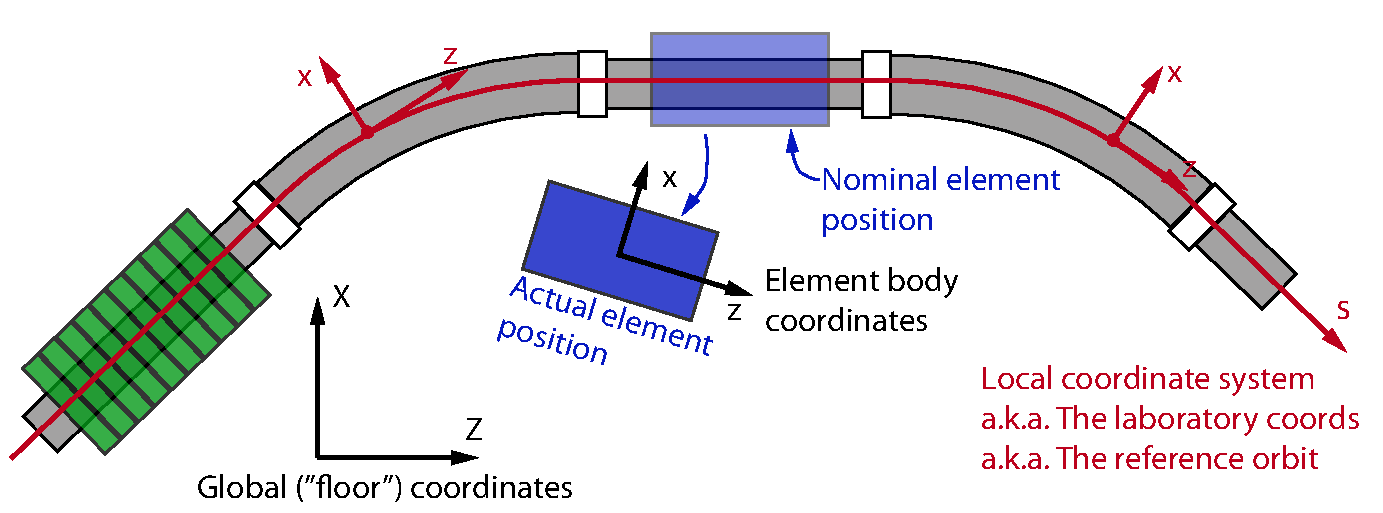
\includegraphics[width=0.9\textwidth]{coordinates.pdf}
  \caption{The three coordinate systems used to describe lattice element positioning:
\vn{Global}, \vn{reference}, and \vn{element body} coordinates.}
  \label{f:coordinates}
\end{figure}

%----------------------------------------------------------
\subsection{Coordinate Systems}
\label{s:coord.sys}

As explained in the \vn{Coordinates} chapter of the \bmad manual, bmad uses three coordinate
systems to describe the positioning of lattice elements as shown in Figure~\ref{f:coordinates}:
\begin{description}
\item[Global Coordinates] \Newline
The \vn{(X, Y, Z)} \vn{global} (also called \vn{floor}) coordinate system (notice that capital
letters are used) is independent of the accelerator machine and is "attached" to the building the
accelerator is in. Typically, the \vn{Y}-axis is taken to be pointing vertically up and \vn{(X, Z)}
is the horizontal plane.
%
\item[Local Coordinates] \Newline
The \vn{global} coordinate system is not convenient for describing where particles are as they move
through the lattice. For this, shown in red, there is the \vn{local} (also called \vn{laboratory},
also called \vn{reference}) curvilinear coordinate system. Laboratory coordinates are also used to
describe the nominal (that is, without any ``misalignments'') position of the lattice elements. The
laboratory coordinates start with a curved line often called the ``\vn{reference trajectory}''. The
distance along the reference trajectory is denoted by $s$. At each point along the reference
trajectory, there is a Cartesian \vn{(x, y, z)} coordinate system with the origin at the reference
trajectory point. The $z$-axis is always tangent to the reference trajectory and the $x$ and
$y$-axes always transverse to the reference trajectory.
%
\item[Element Body Coordinates] \Newline
Elements can be shifted ("misaligned") from their nominal position. To describe things like electric
and magnetic fields or apertures (which can depend upon the elements actual position), \vn{element body}
coordinates are used.  The \vn{element body} coordinates are the coordinates attached to the
physical element. Without any "misalignments", the \vn{element} coordinates correspond to the
\vn{laboratory} coordinates.
\end{description}

\begin{figure}[tb]
  \centering
  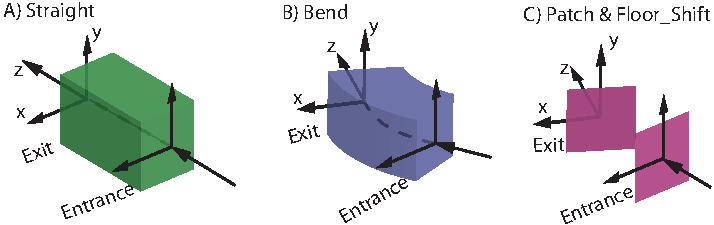
\includegraphics[width=0.9\textwidth]{element-coord-frame.pdf}
  \caption{Lattice element geometry types: \vn{Straight}, \vn{bend}, and \vn{patch}. All elements have an 
\vn{entrance} coordinate system and an \vn{exit} coordinate system.}
  \label{f:body.types}
\end{figure}

%----------------------------------------------------------
\subsection{Element Geometry Types}

All lattice elements have an ``\vn{entrance}'' end and an ``\vn{exit}'' end. Normally a particle
will enter the element at the \vn{entrance} end and exit at the \vn{exit} end but it is possible to
simulate particles going backwards or have lattice elements that are reversed longitudinally.

Lattice elements in \bmad have one of four geometry types. Three of them will be discussed here and
are shown in Figure~\ref{f:body.types}. [The fourth geometry type, used for X-ray simulations, is
used with \vn{mirror}, \vn{multilayer_mirror}, and \vn{crystal} elements.] These three types are
called \vn{straight}, \vn{bend} and \vn{patch} based upon how the $(x, y, z)$ laboratory coordinates
transform as a function of the longitudinal \vn{s} position from the \vn{entrance} end of the
element to the \vn{exit} end.
\begin{description}
\item[Straight Geometry] \Newline
The straight geometry shown in Figure~\ref{f:body.types}A is used with elements like \vn{drifts} and
\vn{quadrupoles}. The orientation of the $(x, y, z)$ coordinates is independent of $s$ and the
reference trajectory is a straight line so that the \vn{z}-axis at the \vn{exit} end is co-linear
with the \vn{entrance} \vn{z}-axis.
\item[Bend Geometry] \Newline
The bend geometry shown in Figure~\ref{f:body.types}B is used with \vn{sbend} and \vn{rbend} dipole
elements. With this geometry, the reference trajectory is a semi-circle. The $(x, y, z)$ coordinates
rotate about an axis which is perpendicular to the $z$-axis. The default is to have the rotation
axis parallel to the $y$-axis which keeps the orientation of the $y$-axis independent of $s$.
\item[Patch Geometry] \Newline 
The patch geometry shown in Figure~\ref{f:body.types}C is used with \vn{patch} and \vn{floor_shift}
elements. With the \vn{patch} geometry, the exit coordinates can be arbitrarily positioned with
respect to the entrance coordinates. See section~\sref{s:patch}. The reference trajectory within the patch
region is undefined since there is no good way to define it.
\end{description}

\newpage

%----------------------------------------------------------
\subsection{Local Coordinate System Construction}

\begin{figure}[tb]
  \centering
  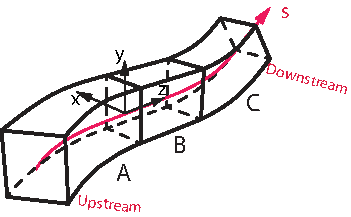
\includegraphics[width=0.6\textwidth]{element-stream.pdf}
  \caption{The \vn{local} coordinate system is constructed by taking the ordered list of lattice elements and
connecting the \vn{exit} frame of one element to the \vn{entrance} frame of the next.}
  \label{f:leggo}
\end{figure}

The \vn{local} coordinate system is constructed by taking the ordered list of lattice elements and
connecting the \vn{(x, y, z)} \vn{exit} frame of one element to the \vn{(x, y, z)} \vn{entrance}
frame of the next (just like LEGO blocks). Given a line constructed as:
\begin{code}
    lat: line = (A, B, C)
\end{code}
The result could look as shown in Figure~\ref{f:leggo}. The reference trajectory is shown in
red.

\newpage

%----------------------------------------------------------
\subsection{Laboratory Coordinates Relative to Global Coordinates}
\label{s:lab.rel.glob}

\begin{figure}[tb]
  \centering
  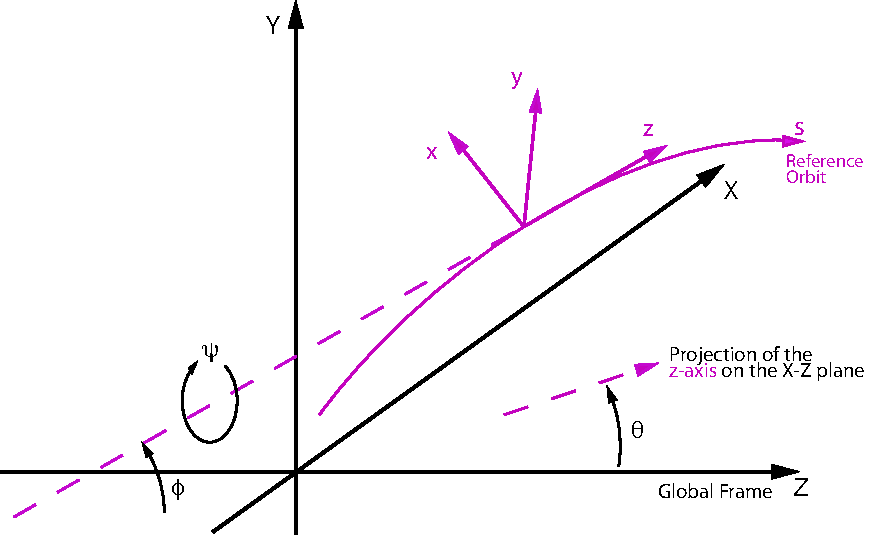
\includegraphics[width=0.9\textwidth]{global-coords.pdf}
  \caption{The global coordinate system.}
  \label{f:global}
\end{figure}

For any given \vn{s}-position on the reference orbit, the \vn{local} coordinate system is described with
respect to the \vn{global} coordinate system by 6 parameters as shown in Figure~\ref{f:global}:
\vspace{-5 pt}
\begin{itemize}
\item (\vn{X}, \vn{Y}, \vn{Z}) global position
\item \vn{$\theta$} azimuth angle in the (X, Z) plane.
\item \vn{$\phi$} elevation angle
\item \vn{$\psi$} roll angle.
\end{itemize}

Notes:
\vspace{-5 pt}
\begin{itemize}
\item 
The default is for the beginning of the lattice (\vn{s} = 0) is to have the local \vn{(x, y, z)}
coordinate system aligned with the global \vn{(X, Y, Z)} coordinate system with $\theta$, $\phi$ and
$\psi$ all being zero.
\item 
For a machine that lies in the horizontal plane, the $\phi(s)$ and $\psi(s)$ angles are zero for all
\vn{s}.
\end{itemize}

\newpage

%----------------------------------------------------------
\subsection{Element Misalignments}
\label{s:ele.mis}

\begin{figure}[tb]
  \centering
  \begin{subfigure}[t]{0.62\textwidth}
    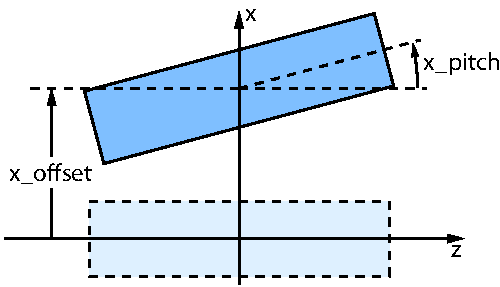
\includegraphics[width=\textwidth]{pitch.pdf}
    \caption{Effect of x_offset and x_pitch on a straight line element}
    \label{f:pitch}
  \end{subfigure}
  \hfil
  \begin{subfigure}[t]{0.33\textwidth}
    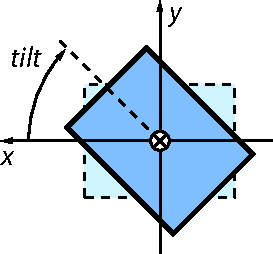
\includegraphics[width=\textwidth]{tilt.pdf}
    \caption{Effect of a tilt on a straight line element.}
    \label{f:tilt}
  \end{subfigure}
  \caption{}
\end{figure}

Once the \vn{reference} coordinate system is established, the position of any physical element
can be shifted (``misaligned''). [Note: \vn{Patch} and \vn{floor_shift} elements cannot be misaligned.]
For straight elements, the element attributes that determine any misalignment are:
\begin{description}
\item[x_offset, y_offset, z_offset] \Newline
The \vn{x_offset}, \vn{y_offset}, and \vn{z_offset} attributes offset the element in the \vn{x}, \vn{y},
and \vn{z} directions respectively. See Figure~\ref{f:pitch}.
%
\item[x_pitch, y_pitch] \Newline
The \vn{x_pitch} and \vn{y_pitch} attributes rotate the element. A \vn{x_pitch} of $\pi/2$ would rotate the
element around the +\vn{y}-axis so that the body +\vn{z}-axis is aligned with the local
+\vn{x}-axis. Similarly, a \vn{y_pitch} of $\pi/2$ would rotate the element around the -\vn{x}-axis so
that the body +\vn{z}-axis is aligned with the local +\vn{y}-axis. See Figure~\ref{f:pitch}.
%
\item[tilt] \Newline
A \vn{tilt} rotates the element around the +\vn{z}-axis as shown in Figure~\ref{f:tilt}
\end{description}

Note: The above only applies to straight elements. Patch like elements are explained below. For a
discussion of misalignments for bend type elements see the \bmad manual.

Example:
\begin{code}
! Lattice File: misalign.bmad
beginning[beta_a] = 10.   ! m  a-mode beta function
beginning[beta_b] = 10.   ! m  b-mode beta function
beginning[e_tot] = 10e6   ! eV
parameter[geometry] = open  ! or closed
q: quadrupole, L = 1, x_offset = 0.1, x_pitch = 0.04
lat: line = (q)   ! List of lattice elements
use, lat          ! Line used to construct the lattice
\end{code}

Start \tao as explained in section~\sref{s:tao.run} with the lattice file \vn{misalign.bmad}. The
misalignment can be viewed using the \vn{-floor} option with the \vn{show element } command:
\begin{code} 
Tao> show ele q -floor

 Element #                1
 Element Name: Q
... etc...

 Attribute values [Only non-zero/non-default values shown]:
    1  L               =  1.0000E+00 m
   13  SPIN_FRINGE_ON  =  T (1)
   31  L_HARD_EDGE     =  1.0000E+00 m
   34  X_PITCH         =  4.0000E-02       55  X_PITCH_TOT   =  4.0000E-02
   36  X_OFFSET        =  1.0000E-01 m     57  X_OFFSET_TOT  =  1.0000E-01 m
... etc...

Global Floor Coords at End of Element:
                X        Y        Z    Theta  
Reference  0.00000  0.00000  1.00000  0.00000 ... ! Without misalignments
Actual     0.11999  0.00000  0.99960  0.04000 ... ! With misalignments
... etc...
\end{code}

In the ``\vn{Global Floor Coords}'' section, the \vn{Reference} row shows the nominal position of
the \vn{exit} end of the element without misalignments. [Due to space constraints the \vn{phi} and
\vn{psi} columns are not shown. They are zero in this case.] The \vn{Actual} row shows the position
of the physical element at the \vn{exit} end.

Associated with each misalignment attribute there is a corresponding attribute with a ``\vn{_tot}''
suffix. The difference is that an attribute like \vn{x_offset} is the misalignment with respect to
any \vn{girder} (\sref{s:girder}) that may be supporting it while the corresponding
\vn{x_offset_tot} is the total misalignment of the lattice element with respect to the element's
nominal position. Another difference is that misalignments attributes are set by the user while the
corresponding \vn{_tot} attributes are calculated by \bmad. If there is no \vn{girder} support, the
\vn{_tot} attributes will be the same as the misalignment attributes as it is in this case so
\vn{x_pitch} is equal to \vn{x_pitch_tot}, etc.

\newpage

\begin{figure}[tb]
  \centering
  \begin{subfigure}[t]{0.48\textwidth}
    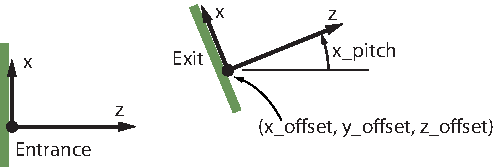
\includegraphics[width=\textwidth]{patch.pdf}
    \vspace*{5pt}
    \caption{The body coordinates at the exit end of a \vn{patch} is set by the element attributes
\vn{x_offset}, \vn{y_offset}, \vn{z_offset}, \vn{x_pitch}, \vn{y_pitch}, and \vn{tilt}.}
    \label{f:patch}
  \end{subfigure}
  \hfil
  \begin{subfigure}[t]{0.48\textwidth}
    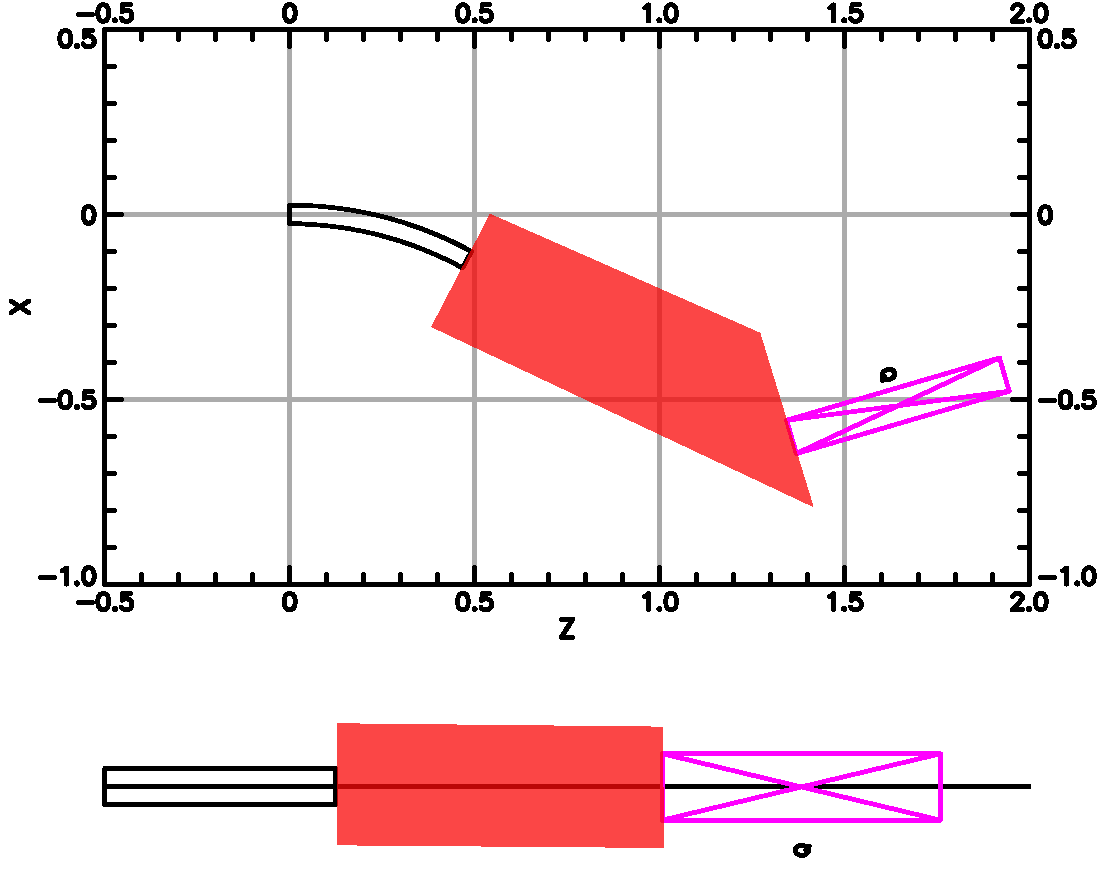
\includegraphics[width=\textwidth]{patch-example.pdf}
    \caption{Lattice with a patch element.
The patch element is the coordinates patch element in a lattice. [Note: The default is not to
draw \vn{patch} elements in a \vn{floor_plan} plot.]}
    \label{f:patch.example}
  \end{subfigure}
  \caption{}
\end{figure}

%----------------------------------------------------------
\subsection{Patch Elements}
\label{s:patch}

\vn{Patch} elements are used to shift the reference orbit. As a consequence, the nominal placements
of all elements downstream of the patch are affected. This is useful in simulating things like injection
or extraction lines where the patch is used to reorient the reference orbit so that it follows the 
injection or extraction line.

For \vn{patch} elements the same six parameters that are used to misalign straight line elements
are, for a \vn{patch}, used to set the placement of the \vn{exit} frame relative to the \vn{entrance}
frame. The transformation from entrance coordinates to exit coordinate is:
\vspace{-5 pt}
\begin{enumerate}
\item Initially the exit coordinates coincide with the entrance coordinates.
\item The origin of the exit coordinates is translated by (\vn{x_offset}, \vn{y_offset}, \vn{z_offset})
\item The \vn{x_pitch} and \vn{y_pitch} rotations (in radians) are applied. 
The \vn{x_pitch} rotation rotates the \vn{+z} axis
towards the \vn{+x} axis (rotation around the +y axis). The \vn{y_pitch} rotation rotates the \vn{+z} axis
towards the \vn{+y} axis (rotation around the -x axis).
\item The \vn{tilt} rotation (in radians) rotates the exit coordinates around the exit coordinate's +z
axis.
\end{enumerate}
This transformation is illustrated in Figure~\ref{f:patch}. The transformation from \vn{patch}
\vn{entrance} to \vn{exit} coordinates is the same transformation from laboratory coordinates at the
center of a straight element to the element body coordinates at the center of the misaligned
element.

\newpage

Example:
\begin{code}
! Lattice File: patch.bmad
beginning[beta_a] = 10.   ! m  a-mode beta function
beginning[beta_b] = 10.   ! m  b-mode beta function
beginning[e_tot] = 10e6   ! eV
parameter[geometry] = open  ! or closed

b: sbend, L = 0.5, g = 1    ! g = 1 / bending_radius
p: patch, z_offset = 1, x_pitch = pi/4
q: quadrupole, L = 0.6, k1 = 0.23

lat: line = (b, p, q)   ! List of lattice elements
use, lat                ! Line used to construct the lattice
\end{code}

Start \tao as explained in section~\sref{s:tao.run} with the lattice file \vn{patch.bmad}. Create a
\vn{floor_plan} with the command \vn{place r11 floor}. The result is shown in
Figure~\ref{f:patch.example} except that, by default, \tao does not draw a patch element so, in the
figure, the patch has been drawn in by hand. The global coordinates of the nominal positions of the
elements can be seen by using the \vn{show lat -floor} command:
\begin{code}
Tao> show lat -floor

      Values at End of Element:
Ix  name      key               s          X         Y         Z     Theta ...
 0  BEGINNING Beginning_Ele  0.000    0.0000    0.0000    0.0000    0.0000 ...
 1  B         Sbend          0.500   -0.1224    0.0000    0.4794   -0.5000 ...
 2  P         Patch          1.207   -0.6018    0.0000    1.3570    0.2854 ...
 3  Q         Quadrupole     1.807   -0.4329    0.0000    1.9327    0.2854 ...
 4  END       Marker         1.807   -0.4329    0.0000    1.9327    0.2854 ...
\end{code}

A \vn{patch} represents a field free space so a particle traveling through a patch propagate as in a
drift. The difference is that in a \vn{patch} there is a coordinate transformation from entrance
coordinates to exit coordinates.

%----------------- 
\subsection{Exercises [Answers in Section \sref{s:ans.coords}]}
\label{s:coords.ex}

\begin{enumerate}[label=\thesection.\arabic{enumi}]
\item
Modify the lattice file \vn{simple.bmad} to include a \vn{girder} element supporting elements \vn{B}
and \vn{Q}. Misalign the \vn{girder} and verify that a supported element will have \vn{_tot}
attributes different from the misalignment attributes.
%
\item
Create a lattice with elements \vn{drift}, followed by a \vn{mirror}, followed by a \vn{drift}.
Give the \vn{mirror} a finite \vn{graze_angle} and verify that the laboratory coordinate after the
\vn{mirror} are rotated by twice the \vn{graze_angle} with respect to the coordinates before the
\vn{mirror} so that a photon traveling on the zero-orbit before the \vn{mirror} will stay on the
zero-orbit after the \vn{mirror}.
%
\item
Using lattice simple.bmad, calculate by hand the floor coordinates at the exit end of element Q and compare this with the coordinates as calculated by Bmad.
\end{enumerate}

\newpage

%------------------------------------------------------------------------------
%------------------------------------------------------------------------------
\Section{Particle Phase Space Coordinates}
\label{s:phase.space}

The previous chapter showed how to describe the placement of lattice elements. This chapter
covers how to describe particle trajectories. 

\begin{figure}[tb]
  \centering
  \begin{subfigure}[t]{0.48\textwidth}
    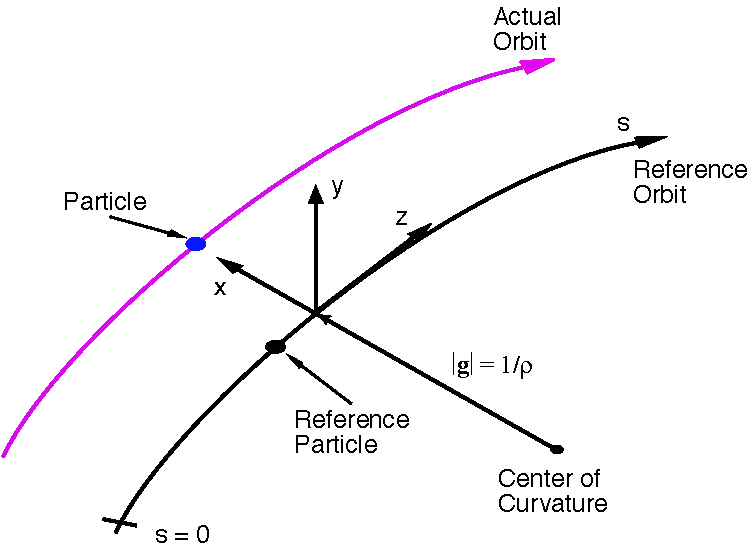
\includegraphics[width=0.9\textwidth]{local-coords.pdf}
    \caption{Particle coordinate positions are relative to the reference orbit.}
    \label{f:part.coords}
  \end{subfigure}
  \hfil
  \begin{subfigure}[t]{0.48\textwidth}
    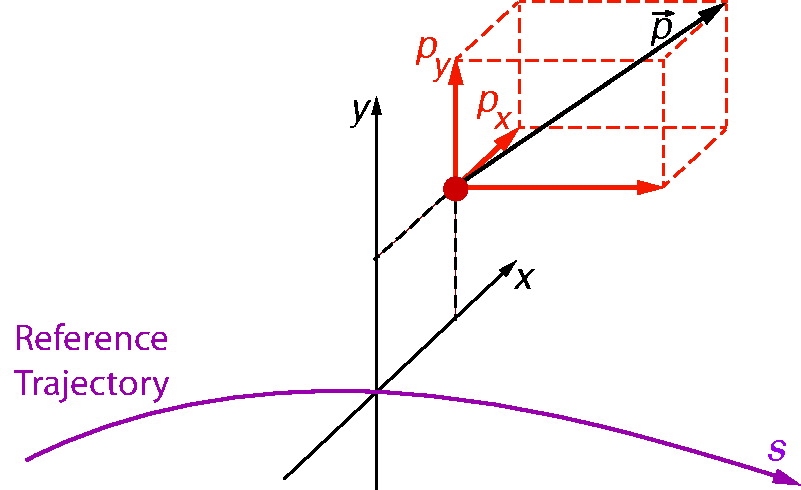
\includegraphics[width=\textwidth]{CoordinateSystem1.pdf}
    \caption{Particle phase space.}
    \label{f:phase.space}
  \end{subfigure}
  \caption{}
\end{figure}

%----------------------------------------------------------
\subsection{Particle Phase Space Coordinates}
\label{s:phase.space.sub}

Figure~\ref{f:part.coords} shows the reference orbit. As explained in the previous chapter, the
reference coordinates $(x, y, z)$ associated with a given point a distance $s$ along the reference
point has the coordinate origin at the given point and the $z$-axis tangent to the reference orbit.

A particle being simulated has its own trajectory as shown in the figure. Given a particle at some
point on its trajectory (blue dot in Figure~\ref{f:part.coords}), there is a point at position
\vn{s} on the reference orbit such that the $z$ coordinate of the particle is zero in the (\vn{x},
\vn{y}, \vn{z}) coordinate frame associated with the reference orbit point.

With this, the particle's position and momentum \vn{P} can be described using the coordinates:
\begin{code}
    (x(s), y(s), Px(s), Py(s), Pz(s), t(s))
\end{code}
where \vn{t(s)} is the time that the particle is at the given point. From now on, to simplify the
notation, the \vn{s} dependence will be dropped.

For tracking purposes, canonical phase space coordinates are used with the convention that upper
case \vn{P} denotes (unnormalized) momentum (Figure~\ref{f:phase.space}) and lower case \vn{p}
denotes phase space momentum. The phase space coordinates are denoted
\begin{code}
    (x, px, y, py, z, pz)
\end{code}
where
\begin{lstlisting}[mathescape]
    px = Px / P0
    py = Py / P0
    pz = (P - P0) / P0
    z  = c * @!\textbeta!@ * (t_ref - t)
\end{lstlisting}
with
\vspace{-5 pt}
\begin{itemize}
\item \vn{P0} is the reference momentum. See section~\sref{s:ref.energy}.
\item \vn{c * \textbeta} is the velocity of the particle, 
\item \vn{t_ref(s)} is the time the reference particle reaches the point \vn{s}. The reference
particle is a fictitious particle that can be imagined to be traveling on the reference orbit.
Frequently, this reference particle is thought of as describing the center of a bunch of particles.
\end{itemize}
Notes:
\vspace{-5 pt}
\begin{itemize}
\item
Do not confuse the canonical \vn{z} coordinate with the \vn{z} coordinate of the particle in the
(\vn{x},~\vn{y},~\vn{z}) coordinate frame. By construction, The latter is always zero.
\item 
For a bunch of particles at a given \vn{s} position, in general, the particles will have differing
time \vn{t}.
\item 
If the reference particle has the same {\textbeta} value as a particle, canonical \vn{z} will be the
longitudinal distance the particle is with respect to the reference particle. Positive \vn{z}
indicates that the particle is in front of the reference particle and vice versa.
\end{itemize}


\begin{figure}[tb]
  \centering
  \begin{subfigure}[t]{0.48\textwidth}
    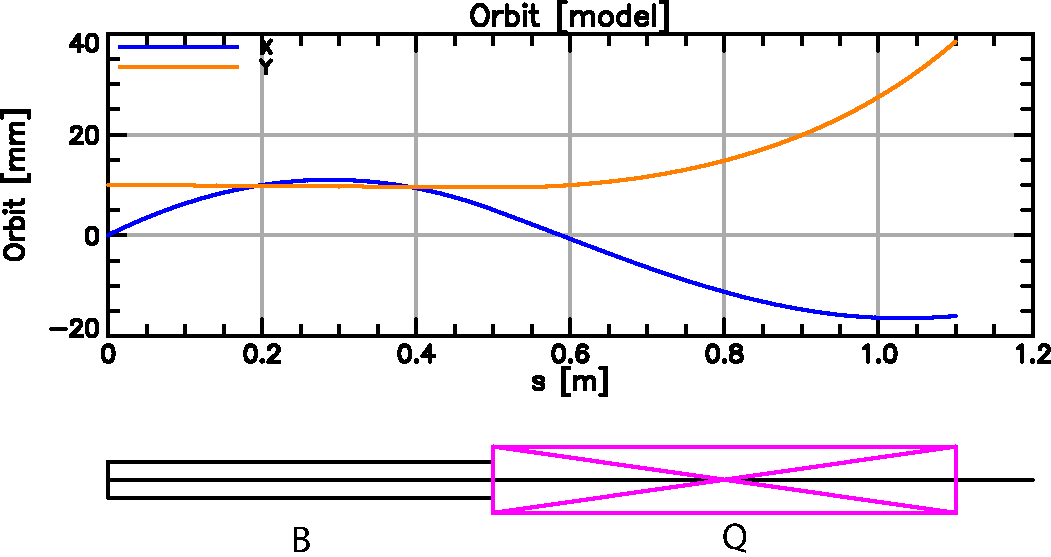
\includegraphics[width=\textwidth]{phase0.pdf}
    \caption{Initial orbit.}
    \label{f:phase0}
  \end{subfigure}
  \hfil
  \begin{subfigure}[t]{0.48\textwidth}
    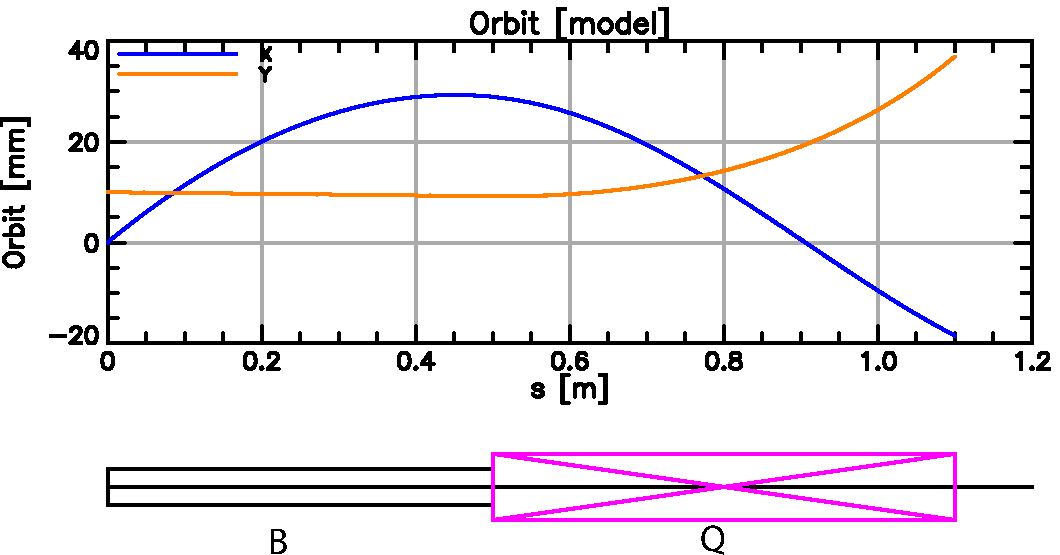
\includegraphics[width=\textwidth]{phase1.pdf}
    \caption{Orbit after adjusting the starting \vn{px} phase space coordinate.}
    \label{f:phase1}
  \end{subfigure}
  \caption{}
\end{figure}

%----------------------------------------------------------
\subsection{Example}

Example lattice:
\begin{code}
! Lattice File: orbit.bmad
beginning[beta_a] = 10.   ! m  a-mode beta function
beginning[beta_b] = 10.   ! m  b-mode beta function
beginning[e_tot] = 10e6   ! eV
parameter[geometry] = open  ! or closed
bmad_com[spin_tracking_on] = T

particle_start[y] = 0.01
particle_start[px] = 0.06
particle_start[pz] = -0.2
particle_start[spin_x] = 1

b: sbend, L = 0.5, g = 1    ! g = 1 / bending_radius
q: quadrupole, L = 0.6, k1 = 10

lat: line = (b, q)   ! List of lattice elements
use, lat                ! Line used to construct the lattice
\end{code}

Start \tao as explained in section~\sref{s:tao.run} with the lattice file \vn{orbit.bmad}. Here
spin tracking is turned on (\vn{bmad_com[spin_tracking_on] = T}) and a non-zero initial orbit is set
using \vn{particle_start} parameters. The resulting orbit is shown in Figure~\ref{f:phase0}.

The initial phase space coordinates can now be varied using the \vn{change} or \vn{set}
commands. For example:
\begin{code}
Tao> change particle_start px 0.04
           Old           New    Old-Design    New-Design         Delta
      0.060000      0.100000      0.000000      0.040000      0.040000  
\end{code}

The result is shown in Figure~\ref{f:phase1}. 

View Orbits with \vn{show lattice} command

\begin{code}
Tao> show lat -spin -orbit
      Values at End of Element:
 Index  name      key           ...           orbit  ...          spin 
                                ...               x  ...             x 
     0  BEGINNING Beginning_Ele ...    0.000000E+00  ...  0.000000E+00 
     1  B         Sbend         ...    5.027722E-03  ... -1.414516E-01 
     2  Q         Quadrupole    ...   -1.599068E-02  ... -7.350543E-02 
     3  END       Marker        ...   -1.599068E-02  ... -7.350543E-02 
\end{code}

or the \vn{show element} command

\begin{code}
Tao> show ele 1
 Element #                1
 Element Name: B
... etc...

Orbit:  Positron   State: Alive
         Position[mm] Momentum[mrad]        Spin   |
  X:       5.02772161   -44.34051580  -0.14145163  | Particle [sec]:     ...
  Y:       9.52710654    -1.27804602  -0.00171549  | Part-Ref [sec]:     ...
  Z:      -4.78648430  -200.00000000   0.98994368  | (Ref-Part)*Vel [m]: ...
\end{code}

%----------------------------------------------------------
\subsection{Reference Energy and the Lcavity and RFcavity Elements}
\label{s:ref.energy}

Every lattice element has a reference particle, a reference energy called \vn{E_tot}, and a
reference momentum named \vn{p0c} (in eV). The three are interrelated so knowing the reference
particle and either the reference momentum or energy, the third quantity can be calculated. The
reference momentum is used for normalization of the phase space momentum (\sref{s:phase.space.sub})
as well as normalized strength parameters. For example, for a quadrupole element, the
\vn{b1_gradient} parameter (units: Tesla/m) can be used to specify the linear field gradient and the
\vn{k1} parameter (units: 1/m$^2$) is the normalized field gradient normalized using the value of
the reference momentum as discussed in the ``\vn{Magnetostatic Multipole Fields}'' section of the
``\vn{Electromagnetic Fields}'' chapter of the \bmad manual.

For lattices with an \vn{open} geometry (\sref{s:lat.geom}), the reference energy/momentum at the
beginning of the lattice is what is set in the lattice file. The reference energy/momentum for a
downstream element inherits the reference energy/momentum of the element just upstream. The exception
is for \vn{Lcavity} elements, which represent an RF cavity, where the reference energy/momentum at
the exit end of the \vn{lcavity} is set so that a particle entering the cavity with zero phase space
coordinates leaves with zero phase space coordinates and in particular phase space \vn{pz} will be
zero at the exit end. \vn{Lcavity} elements also have \vn{p0c_start} and \vn{E_tot_start} parameters
that are set to the reference energy of the upstream element. Notice that with \vn{rfcavity}
elements, which also represent an RF cavity, the reference energy/momentum is the same as the
upstream element. Example:
\begin{code}
! Lattice File: cavity.bmad
beginning[beta_a] = 10.   ! m  a-mode beta function
beginning[beta_b] = 10.   ! m  b-mode beta function
beginning[p0c] = 1e8   ! eV  

parameter[geometry] = open      ! or closed
parameter[particle] = He+ 

q1: quad, l = 0.1, k1 = 0.14
q2: quad, l = 0.1, b1_gradient = parameter[p0c] * q1[k1] / c_light
lc: lcavity, l = 1, voltage = 10e8, rf_frequency = 1e9
rf: rfcavity, l = 1, voltage = 10e8, phi0 = 0.25

lat: line = (q1, q2, lc, q1, q2, rf)
use, lat
\end{code}

Notes:
\vspace{-5 pt}
\begin{itemize}
\item For a \vn{lcavity} phi0 = 0 corresponds to peak acceleration.
\item For an \vn{rfcavity} phi0 = 0.25 corresponds to peak acceleration.
\end{itemize}

Start \tao as explained in section~\sref{s:tao.run} with the lattice file
\vn{cavity.bmad}. Examining the \vn{lcavity} element shows:
\begin{code}
> tao -lat cavity.bmad

Tao> show ele 3
Element #                3
Element Name: LC
Key: Lcavity
... etc...
   51   P0C_START    =  1.000000E+08 eV        BETA_START   =  0.02681151
   52   E_TOT_START  =  3.729740E+09 eV        DELTA_E      =  1.000000E+09 eV
   53   P0C          =  2.910237E+09 eV        BETA         =  0.61530588
   54   E_TOT        =  4.729740E+09 eV        GAMMA        =  1.268571E+00
... etc...    
Orbit:  He+   State: Alive
         Position[mm] Momentum[mrad]        Spin   |
  X:       0.00000000     0.00000000               | Particle [sec]:     ...
  Y:       0.00000000     0.00000000               | Part-Ref [sec]:     ...
  Z:      -0.00000000     0.00000000               | (Ref-Part)*Vel [m]: ...
\end{code}

The reference energy at the start of the element, \vn{E_tot_start}, is not the same as the reference
energy at the end of the element \vn{E_tot}. The particle orbit, which started out with zero phase
space coordinates (there were no \vn{particle_start} statements to give a non-zero starting orbit), still
has zero phase space coordinates at the end of the \vn{lcavity} element.


Compare this to the \vn{rfcavity} element:
\begin{code}
Tao> show ele 6
Element #                6
Element Name: RF
Key: RFcavity
... etc...
   53   P0C         =  2.9102374E+09 eV         BETA      =  0.615305883
   54   E_TOT       =  4.7297409E+09 eV         GAMMA     =  1.2685712E+00
... etc...
 Orbit:  He+   State: Alive
         Position[mm] Momentum[mrad]        Spin   |
  X:       0.00000000     0.00000000               | Particle [sec]:     ...
  Y:       0.00000000     0.00000000               | Part-Ref [sec]:     ...
  Z:     140.37425587   494.97867675               | (Ref-Part)*Vel [m]: ...
\end{code}

Here there is no \vn{E_tot_start} parameter since the ending reference energy is always equal to the
starting one. Here, the \vn{pz} coordinate at the end of the element is nonzero.

%------------------------------------------------------------------------------
\subsection{Exercises [Answers in Section \sref{s:ans.phase}]}
\label{s:phase.space.ex}

\begin{enumerate}[label=\thesection.\arabic{enumi}]
\item 
Modify the \vn{lcavity} in the \vn{cavity.bmad} to have a small length (so the transit time is
small), and set the beginning momentum small enough so the relativistic beta is significantly than
one. Starting the particle with a finite $z$, calculate the ending $z$ after the cavity and verify
that the range in $z$ is consistent with the equation for $z$ given in \sref{s:phase.space.sub}.
%
\item
\vn{Lcavity} elements have an attribute \vn{phi0_err} which varies the RF phase that a particle sees
but does not change the reference energy. Add a finite \vn{phi0_err} to the \vn{cavity} element and
verify that the reference energy does not change but that the phase space \vn{pz} of the particle
(which is the normalized momentum deviation from the reference \sref{s:phase.space.sub}) does
change. With the \vn{cavity.bmad} lattice, there is a range of values for \vn{phi0_err} where the
cavity will decelerate the particle enough so that the particle will turn around and not make
it through the cavity. Approximately what is this range?
\end{enumerate}

\newpage

%------------------------------------------------------------------------------
%------------------------------------------------------------------------------
\Section{Superposition}
\label{s:super}

\vn{Superposition} is used when elements overlap spatially. In such a case, \bmad creates
``\vn{slave}'' elements that will be tracked through and ``\vn{lord}'' elements that represent the
individual elements.  Some examples will make this clear. Note: Superposition is discussed in the
``Superposition'' chapter in the Bmad manual.

\begin{figure}[b]
  \centering
  \includegraphics[width=0.9\textwidth]{superimpose.pdf}
  \caption{The placement of superimposed elements is determined by an offset from a reference element.}
  \label{f:superimpose}
\end{figure}

%----------------------------------------------------------
\subsection{Example 1}

Superposition works by defining a \vn{line} as done in any lattice file and then defining an element
that will be ``superimposed'' on top of the line. To superimpose an element you need to specify
where the element is placed. To do this, a reference position is specified and the superimposed
element is placed at that position shifted by a specified offset as illustrated in
Figure~\ref{f:superimpose}. The lattice file \vn{superimpose1.bmad} illustrates how superposition is
done.
\begin{code}
! Lattice File: superimpose1.bmad

beginning[beta_a] = 10.   ! m  a-mode beta function
beginning[beta_b] = 10.   ! m  b-mode beta function
beginning[e_tot] = 10e6   ! eV   Or can set p0c
parameter[geometry] = open      ! or closed

q: quadrupole, L = 1, k1 = 0.2
d: drift, L = 1

m1: marker, superimpose, ref = q, ref_origin = beginning, offset = 0.3
m2: marker, superimpose, ref = q, ref_origin = end, offset = 0.4

lat: line = (q, d)   ! List of lattice elements
use, lat             ! Line used to construct the lattice
\end{code}
Here two marker elements named \vn{m1} and \vn{m2} are superimposed on the lattice. The offsets for
\vn{m1} and \vn{m2} are 0.3 meters and 0.4 meters respectively. The reference position is determined
by the reference element, which is specified by the \vn{ref} attribute, and the \vn{ref_origin}
attribute which specifies where on the reference element the reference position is. In this example,
the reference point for \vn{m1} is the \vn{beginning} (upstream) end of element \vn{q} and the
reference point for \vn{m2} is the (downstream) \vn{end} of element \vn{q}. The element origin is
similarly defined using the \vn{ele_origin} attribute. In this case, since marker elements have zero
length, the setting of \vn{ele_origin} is immaterial.

Start \tao as explained in section~\sref{s:tao.run} with the lattice file
\vn{superimpose1.bmad}. The lattice looks like:

\begin{code}
Tao> show lat
      Values at End of Element:
 Index  name      key                     s       l    beta     phi    eta ...
                                                          a       a      a ...
     0  BEGINNING Beginning_Ele       0.000     ---   10.00   0.000   0.00 ...
     1  Q#1       Quadrupole          0.300   0.300    9.83   0.030   0.00 ...
     2  M1        Marker              0.300   0.000    9.83   0.030   0.00 ...
     3  Q#2       Quadrupole          1.000   0.700    8.22   0.107   0.00 ...
     4  D#1       Drift               1.400   0.400    6.97   0.160   0.00 ...
     5  M2        Marker              1.400   0.000    6.97   0.160   0.00 ...
     6  D#2       Drift               2.000   0.600    5.37   0.258   0.00 ...
     7  END       Marker              2.000   0.000    5.37   0.258   0.00 ...
 Lord Elements:
     8  Q         Quadrupole          1.000   1.000    8.22   0.107   0.00 ...
 Index  name      key                     s       l    beta     phi    eta ...
                                                          a       a      a ...
      Values at End of Element:
\end{code}

The quadrupole \vn{Q} has been split by marker \vn{M1} and so has become a \vn{super_lord} element:
\begin{code}
Tao> show ele Q

 Element #                8
 Element Name: Q
 Key: Quadrupole
... etc...

Slave_status: Free
Lord_status:  Super_Lord
Slaves:
   Index   Name        Type
       1   Q#1         Quadrupole
       3   Q#2         Quadrupole
\end{code}

The two \vn{super_slaves} of \vn{Q}, elements \vn{Q\#1} and \vn{Q\#2}, will be used when tracking a
particle through the lattice.

If parameters of element \vn{Q} are modified, Bmad bookkeeping routines will automatically update the super_slaves.
Thus if the \vn{k1} attribute of \vn{Q} is modified:
\begin{code}
Tao> change ele Q k1 0.11
           Old           New    Old-Design    New-Design         Delta
      0.200000      0.310000      0.110000      0.110000      0.110000    Q
\end{code}

The change will be reflected in the slave elements:

\begin{code}
Tao> show ele 1
 Element #                1
 Element Name: Q#1
 Key: Quadrupole

 Attribute values [Only non-zero/non-default values shown]:
    1   L                            =  3.0000000E-01 m
    4   K1                           =  3.1000000E-01 1/m^2
... etc...

Slave_status: Super_Slave
Associated Super_Lord(s):
   Index   Name                             Type
       8   Q                                Quadrupole
Lord_status:  Not_a_Lord
\end{code}

Parameter values of the super_slave elements are determined by the super_lord and may not be directly set:
\begin{code}
Tao> change ele Q#1 k1 0.01

[ERROR | 2017-AUG-28 22:38:36] tao_change_ele:
    ATTRIBUTE NOT FREE TO VARY. NOTHING DONE
\end{code}

Notes:
\vspace{-5 pt}
\begin{itemize}
\item
The default value for \vn{ref_origin} and \vn{ele_origin}, if not present, is \vn{center} --- the center of
the element.
\item
The default reference element if \vn{ref} is not present is the zero length \vn{beginning} element
at the beginning of the lattice.
\item
With closed lattices (\sref{s:lat.geom}), a superimposed element may "wrap" around so that part of
the superimposed element is at the end of the lattice and part of the element is at the beginning of
the lattice. See the example in Section~\sref{s:lat.geom}.
\item
No super_lord element is made when a drift element is split. Thus in the above example, there is no
\vn{D} super_lord and the two elements \vn{D\#1} and \vn{D\#1} are {\em not} \vn{super_slaves}.
Drifts are the only type of element where, if split, a super_lord element is not created. This is done
to simplify the lattice. If you don't want this behavior, use a \vn{pipe} in place of a \vn{drift}.
\end{itemize}

\newpage

%----------------------------------------------------------
\subsection{Example 2}

The second superposition example involves superposition of an element with finite length:
\begin{code}
! Lattice File: superimpose2.bmad
beginning[beta_a] = 10.   ! m  a-mode beta function
beginning[beta_b] = 10.   ! m  b-mode beta function
beginning[e_tot] = 10e6   ! eV   Or can set p0c
parameter[geometry] = open      ! or closed

Q: quad, l = 4
D: drift, l = 12
S: solenoid, l = 8, superimpose, ref = Q, ele_origin = beginning
M: marker, superimpose, ref = S, offset = 1

lat: line = (Q, D)
use, lat
\end{code}

The superimposes a solenoid on top of a quadrupole and a drift.  
Start \tao as explained in section~\sref{s:tao.run} with the lattice file
\vn{superimpose2.bmad}.

\begin{code}
Tao> show lat
      Values at End of Element:
 Index  name      key                     s       l    beta     phi    eta ...
                                                          a       a      a ...
     0  BEGINNING Beginning_Ele       0.000     ---   10.00   0.000   0.00 ...
     1  Q#1       Quadrupole          2.000   2.000   10.40   0.197   0.00 ...
     2  Q\S       Sol_Quad            4.000   2.000   11.60   0.381   0.00 ...
     3  S#1       Solenoid            7.000   3.000   14.90   0.611   0.00 ...
     4  M         Marker              7.000   0.000   14.90   0.611   0.00 ...
     5  S#2       Solenoid           10.000   3.000   20.00   0.785   0.00 ...
     6  D#1       Drift              16.000   6.000   35.60   1.012   0.00 ...
     7  END       Marker             16.000   0.000   35.60   1.012   0.00 ...
Lord Elements:
     8  Q         Quadrupole          4.000   4.000   11.60   0.381   0.00 ...
     9  S         Solenoid           10.000   8.000   20.00   0.785   0.00 ...
 Index  name      key                     s       l    beta     phi    eta ...
                                                          a       a      a ...
      Values at End of Element:
\end{code}
The \vn{Q\B S} super_slave element has both quadrupole \vn{Q} and solenoid \vn{S} elements as super_lords.
This makes \vn{Q\B S} a \vn{sol_quad} or combination solenoid and quadruple element.

\newpage

\begin{code}
Tao> show ele q\s
 Element #                2
 Element Name: Q\S
 Key: Sol_Quad
... etc...

Slave_status: Super_Slave
Associated Super_Lord(s):
   Index   Name                             Type
       8   Q                                Quadrupole
       9   S                                Solenoid
Lord_status:  Not_a_Lord
\end{code}

Notes:
\vspace{-5 pt}
\begin{itemize}
\item 
This superposition works since Bmad has a \vn{sol_quad} element which is a combination
solenoid/quadrupole. On the other hand, \bmad does not have a combination quadrupole/sextupole element.
When a quadrupole is superimpose with a sextupole the result is an \vn{em_field} element and the
tracking method (\sref{s:methods}) is switched to \vn{runge_kutta}.
\item
\vn{Jumbo} superposition can be used to superimpose elements whose combination cannot be
represented by a corresponding \bmad element. The drawback in this case is that the particle
tracking through this element must be done via a Runge-Kutta or similar tracking
method. (\sref{s:methods}). See the \bmad manual for more details.
\end{itemize}

%------------------------------------------------------------------------------
\subsection{Exercises [Answers in Section \sref{s:ans.super}]}
\label{s:super.ex}

\begin{enumerate}[label=\thesection.\arabic{enumi}]
\item
Create a lattice with a sextupole superimposed in the middle of a quadrupole. Make the length of the 
sextupole shorter than the length of the quadrupole. Make a second lattice similar to the first but
this time use \vn{jumbo} superposition. Compare both lattices.
\end{enumerate}

\newpage

%------------------------------------------------------------------------------
%------------------------------------------------------------------------------
\Section{Multipass}
\label{s:multipass}

Some lattices have the beam recirculating through the same element multiple times. For example, an
Energy Recovery Linac (ERL) will circulate the beam back through the LINAC part to retrieve the
energy in the beam. In \bmad, this situation can be simulated using the concept of \vn{multipass}.
Another situation where multipass is useful is for modeling the interaction region in a colliding
beam machine. In the Bmad manual multipass is discussed in the ``Multipass''
chapter.

%----------------------------------------------------------
\subsection{What is Multipass and What is it Good For?}

Consider the following lattice:
\begin{code}
A: quadrupole
ll: line = (A, A)
use, ll
\end{code}
The lattice has two quadrupoles both called \vn{A}. These two elements, even though they have the
same name, are independent:
\begin{code}
Tao> change ele 1    k1 0.01   ! Can modify first A element.
Tao> change ele A##2 k1 0.02   ! And can modify second A ele independently.
\end{code}
Now consider an ERL. With an ERL, the beam will go through the linac section multiple times. An ERL
lattice might look like:
\begin{code}
linac: line = (...)
arc: line = (...)
dump: line = (..)
erl_line: line = (injector, linac, arc, linac, dump)
\end{code}
Here you don't want the elements of the fist \vn{linac} in \vn{erl_line} to be treated as separate
from the second \vn{linac} in \vn{erl_line} since they represent the same set of physical elements.
This is where \vn{multipass} comes in.  Multipass is used to describe the situation where multiple
elements to be tracked through are actually the same physical element and you want that fact to
be enforced when element parameters are varied.

In this case, the solution is to mark the \vn{linac} line as multipass to tell Bmad that the first
instance of \vn{linac} in \vn{erl_line} contains the same physical elements as the second instance
of \vn{linac}:
\begin{code}
linac: line[multipass] = (...)
\end{code}

With a \vn{multipass} line, \bmad will setup appropriate multipass lords and multipass slaves to
connect together all elements which represent the same physical element.

\newpage

%----------------------------------------------------------
\subsection{Example}

\begin{code}
! Lattice File: multipass.bmad

beginning[beta_a] = 100.   ! m  a-mode beta function
beginning[beta_b] = 100.   ! m  b-mode beta function
beginning[p0c] = 10e6   ! eV   
parameter[geometry] = open      ! or closed

cavity: lcavity, l = 1, voltage = 10e6, rf_frequency = 1e9

linac: line[multipass] = (cavity)
erl: line = (linac, linac) 
use, erl

expand_lattice                
cavity\2[phi0_multipass] = 0.5
\end{code}

Start \tao as explained in section~\sref{s:tao.run} with the lattice file
\vn{multipass.bmad}. The lattice looks like:

\begin{code}
Tao> show lat
      Values at End of Element:
 Index  name       key                   s       l    beta     phi    eta ...
                                                         a       a      a ...
     0  BEGINNING  Beginning_Ele     0.000     ---  100.00   0.000   0.00 ...
     1  CAVITY\1   Lcavity           1.000   1.000   78.87   0.011  -0.00 ...
     2  CAVITY\2   Lcavity           2.000   1.000   42.09   0.028  -0.00 ...
     3  END        Marker            2.000   0.000   42.09   0.028  -0.00 ...
Lord Elements:
     4  CAVITY     Lcavity           0.000   1.000    0.00   0.000   0.00 ...
 Index  name       key                   s       l    beta     phi    eta ...
                                                         a       a      a ...
  Values at End of Element:
\end{code}

Bmad creates a \vn{multipass_lord} called \vn{cavity} to control the \vn{multipass_slaves} called
\vn{cavity\B1} and \vn{cavity\B2}:
\begin{code}
Tao> show ele 4
 Element #                4
 Element Name: CAVITY
... etc...
Slave_status: Free
Lord_status:  Multipass_Lord
Slaves:
   Index   Name        Type
       1   CAVITY\1    Lcavity
       2   CAVITY\2    Lcavity
\end{code}

Since the \vn{cavity} element represents the physical element, any change in the parameters of \vn{cavity}
will be be reflected in the slaves (just like superposition lords and slaves). As an example, changing
the attribute of the lord:
\begin{code}
Tao> set ele cavity x_offset = 0.001
\end{code}
changes the corresponding attributes of the slaves:
\begin{code}
Tao> show ele 2
 Element #                2
 Element Name: CAVITY\2
 Key: Lcavity
 S_start, S:    1.000000,    2.000000
 Ref_time:  6.675633E-09

 Attribute values [Only non-zero/non-default values shown]:
    1   L          =  1.000E+00 m
... etc...
   36   X_OFFSET   =  1.000E-03 m        57   X_OFFSET_TOT  =  1.000E-03 m
... etc...
\end{code}

The exception to the rule that the multipass_lord completely controls the multipass_slave attributes
is the \vn{phi0_multipass} attribute of \vn{lcavity} and \vn{rfcavity} elements. \vn{phi0_multipass}
allows for different settings of the RF phase for different passes through the cavity element.
From the above lattice:
\begin{code}
expand_lattice                 ! cavity\2 is created during lattice expansion
cavity\2[phi0_multipass] = 0.5 ! Shifts the RF phase for cavity\2 by 180^deg
\end{code}
The \vn{expand_lattice} command ``expands'' the lattice to create \vn{cavity\B2} (see the \bmad
manual for more details) and the next line shifts the phase of \vn{cavity\B2} by 180 degrees.

This 180 degrees phase shift makes \vn{cavity\B2} decelerating instead of accelerating. Thus the
reference energy after cavity \vn{cavity\B2} will be the same as the reference energy at the start
of the lattice:
\begin{code}
Tao> show lat -attrib e_tot
      Values at End of Element:
 Index  name      key                      s       l           e
                                                             tot
     0  BEGINNING Beginning_Ele        0.000     ---  1.0013E+07
     1  CAVITY\1  Lcavity              1.000   1.000  2.0013E+07
     2  CAVITY\2  Lcavity              2.000   1.000  1.0013E+07
     3  END       Marker               2.000   0.000  1.0013E+07
Lord Elements:
     4  CAVITY    Lcavity              0.000   1.000  2.0013E+07
 Index  name      key                      s       l           e
                                                             tot
\end{code}

Notes:
\vspace{-5 pt}
\begin{itemize}
\item 
Bmad does not demand that the global position of the multipass_slaves of a multipass_lord be in
the same position in the global coordinate system.
\item
Since the reference energy is changing, the transfer matrix through a \vn{lcavity} will
not be symplectic.
\end{itemize}

\newpage

%------------------------------------------------------------------------------
\subsection{Exercises [Answers in Section \sref{s:ans.multi}]}
\label{s:multipass.ex}

\begin{enumerate}[label=\thesection.\arabic{enumi}]
\item
Modify \vn{multipass.bmad} so that there are two element in the \vn{linac} line called \vn{cavity} and
verify that \bmad does the proper bookkeeping (that is, there are two \vn{cavity} multipass lords.
\end{enumerate}

\newpage

%------------------------------------------------------------------------------
%------------------------------------------------------------------------------
\Section{Lattice Geometry}
\label{s:lat.geom}

The \vn{parameter[geometry]} parameter in a lattice file sets the lattice topology to be
\vn{open} or \vn{closed}:
\vspace*{-20pt}
\begin{description}
\item \vn{open} \Newline 
For \vn{open} lattices, \bmad computes the reference orbit and Twiss parameters by taking the
\vn{beginning[...]} Twiss and \vn{particle_start[...]} orbit settings as the initial values and
propagates them to the end of the lattice (like you would do for a linac).
\item \vn{closed} \Newline 
For \vn{closed} lattices, \bmad calculates the Twiss and orbit periodic solution (like you would in
a storage ring).  In this case, \bmad will ignore Twiss and orbit settings in the lattice file.
\end{description}

\begin{figure}[tb]
  \centering
  \includegraphics[width=0.45\textwidth]{geometry.pdf}
  \caption{\bmad computes the periodic Twiss and orbits for \vn{closed} lattices.}
  \label{f:geometry}
\end{figure}

Example:
\begin{code}
! Lattice File: geometry.bmad
parameter[p0c] = 1e9
parameter[geometry] = closed

d: drift, l = 2
q1: quad, l = 0.5, k1 = 3, hkick = 0.001, superimpose
q2: quad, l = 0.5, k1 = -3, vkick = 0.002, superimpose, offset = 1

lat: line = (d)
use, lat
\end{code}

The lattice looks like:
\begin{code}
Tao> show lat
      Values at End of Element:
 Index  name      key                     s       l    beta     phi    eta ...
                                                          a       a      a ...
     0  BEGINNING Beginning_Ele       0.000     ---    5.93   0.000   0.00 ...
     1  Q1#2      Quadrupole          0.250   0.250    5.57   0.043   0.00 ...
     2  D#1       Drift               0.750   0.500    4.32   0.145   0.00 ...
     3  Q2        Quadrupole          1.250   0.500    4.32   0.266   0.00 ...
     4  D#2       Drift               1.750   0.500    5.57   0.368   0.00 ...
     5  Q1#1      Quadrupole          2.000   0.250    5.93   0.411   0.00 ...
     6  END       Marker              2.000   0.000    5.93   0.411   0.00 ...
Lord Elements:
     7  Q1        Quadrupole          0.250   0.500    5.57   0.043   0.00 ...
 Index  name      key                     s       l    beta     phi    eta ...
                                                          a       a      a ...
\end{code}

The result is shown in Figure~\ref{f:geometry}. The \vn{q1} quadrupole has been superimposed
placing its center at the origin \vn{s} = 0. This results in \vn{q1} being ``wrapped around''
so that first half of \vn{q1}, \vn{q1\#1}, comes at the {\em end} of the tracking part of the lattice
and the second half, \vn{q1\#2}, comes at the beginning of the lattice:
\begin{code}
Tao> show ele q1
 Element #                7
 Element Name: Q1
 Key: Quadrupole
 S_start, S:    1.750000,    0.250000
... etc...

Slave_status: Free
Lord_status:  Super_Lord
Slaves:
   Index   Name        Type
       5   Q1#1        Quadrupole
       1   Q1#2        Quadrupole
\end{code}

Notes:
\vspace{-5 pt}
\begin{itemize}
\item 
Bmad does not demand that a closed lattice be closed in the sense that the global position at the
end of the lattice be the same as the beginning. This makes sense since sometimes you want to take
a lattice section and get the periodic solutions even though the section is not physically closed.
\end{itemize}

\newpage

%------------------------------------------------------------------------------
\subsection{Exercises [Answers in Section \sref{s:ans.geom}]}
\label{s:lat.geom.ex}

\begin{enumerate}[label=\thesection.\arabic{enumi}]
\item
It is sometimes convenient to switch the lattice geometry from closed to open while maintaining the
same beginning Twiss and orbit values. Create an open geometry lattice from the \vn{geometry.bmad}
lattice. While it is possible to code the beginning Twiss and orbit values by hand, an easier way is
to have \tao write a bmad lattice file using the \vn{write bmad} command. This new file will contain
the proper settings for the beginning Twiss and orbit.
%
\item
There is another way to change the geometry besides creating a new lattice file and that is to use
the \vn{set branch} command (see chapter~\sref{s:fork} for an explanation of branches). Run tao and
experiment changing the geometry of the \vn{geometry.bmad} lattice.
\end{enumerate}

\newpage

%------------------------------------------------------------------------------
%------------------------------------------------------------------------------
\Section{Forks and Branches}
\label{s:fork}

A \vn{fork} or \vn{photon_fork} element marks the point where multiple lines can merge or branch off
from. Forking elements can be used to describe such things as X-ray lines branching from storage
rings (see Figure~\ref{f:fork}), injection or extraction lines, etc.

\begin{figure}[tb]
  \centering
  \begin{subfigure}[t]{0.48\textwidth}
    \includegraphics[width=\textwidth]{x-fork.pdf}
    \caption{Fork elements can be used to construct interconnected lines like x-ray lines branching
      from a storage ring.}
    \label{f:fork}
  \end{subfigure}
  \hfil
  \begin{subfigure}[t]{0.48\textwidth}
    \includegraphics[width=\textwidth]{fork-example.pdf}
    \caption{Simple fork example.}
    \label{f:fork.example}
  \end{subfigure}
  \caption{}
\end{figure}

%----------------------------------------------------------
\subsection{Example}

\begin{code}
! Lattice File: fork.bmad

beginning[beta_a] = 10.0        ! m  a-mode beta function
beginning[beta_b] = 10.0        ! m  b-mode beta function
beginning[e_tot] = 10e6         ! eV 
parameter[geometry] = open      ! or closed

b: sbend, l = 2, angle = pi/3
f: fork, to_line = extract_line, superimpose, offset = 0.4
q quadrupole, l = 2

extract_line: line = (q)       ! The line forked to.
extract_line[geometry] = open

lat: line = (b)
use, lat                ! Line used to construct the lattice
\end{code}

In this example The \vn{lat} line is used as the basis for the lattice due to the ``\vn{use, lat}''
statement.  This line contains the bend \vn{b} and, via superposition, the fork element \vn{f}. The
fork element \vn{f} connects to the \vn{to_line} called \vn{extract_line} which contains a single 
quadrupole element called \vn{q}. 

To see the geometry of the lattice, start \tao as explained in section~\sref{s:tao.run} with the
lattice file \vn{fork.bmad} and create a \vn{floor_plan} plot:
\begin{code}
Tao> place r11 floor
\end{code}

The result is shown in Figure~\ref{f:fork.example}.The \vn{fork} element is the red circle.
The lattice is looks like:
\begin{code}
Tao> show lat
      Values at End of Element:
 Index  name      key                     s       l    beta     phi    eta ...
                                                          a       a      a ...
     0  BEGINNING Beginning_Ele       0.000     ---   10.00   0.000   0.00 ...
     1  B#1       Sbend               0.400   0.400    9.77   0.040   0.03 ...
     2  F         Fork                0.400   0.000    9.77   0.040   0.03 ...
     3  B#2       Sbend               2.000   1.600    5.32   0.249   0.75 ...
     4  END       Marker              2.000   0.000    5.32   0.249   0.75 ...
Lord Elements:
     5  B         Sbend               2.000   2.000    5.32   0.249   0.75 ...
 Index  name      key                     s       l    beta     phi    eta ...
                                                          a       a      a ...
      Values at End of Element:
\end{code}

The \vn{show lat} output does not show \vn{q}. Where is the line that was forked to? The answer is
that Bmad creates a set of \vn{branches} to hold the different lines. Branches are assigned an index
starting from 0 and information on them can be seen with the \vn{show branch} command:
\begin{code}
Tao> show branch
                    N_ele  N_ele   ...              Live
  Branch            Track    Max   ...    Geometry  Branch  From_Fork
  0: LAT                4      5   ...    Open       T
  1: EXTRACT_LINE       2      2   ...    Open       T      0>>2
 
                                                                    Defines
  Fork_Element      Forking_To                         Direction    To_Branch?
  0>>2: LAT>>F      1>>0: EXTRACT_LINE>>BEGINNING        1             T
\end{code}  
This shows that the lattice has two branches. When there are multiple branches, elements
are indexed using the notation:
\begin{code}
branch_index>>element_index
\end{code}
so that, for example, ``\vn{0}$>>$\vn{2}'' represents element number 2 in branch 0. That is, the
fork element \vn{f}. 

Each branch has its own set of parameters like the geometry, reference energy, etc. These may be set
using the syntax
\begin{code}
  branch_name[parameter] = ...
\end{code}
For example the ``\vn{extract_line[geometry]}'' was used to set the geometry of \vn{extract_line} in
\vn{fork.bmad}.

The \vn{show lat} branch, by default, shows branch 0. To see other branches use the \vn{-branch} option:
\begin{code}
Tao> show lat -branch 1
      Values at End of Element:
 Index  name      key                     s       l    beta     phi    eta ...
                                                          a       a      a ...
     0  BEGINNING Beginning_Ele       0.000     ---    9.77   0.040   0.03 ...
     1  D         Drift               2.000   2.000    8.04   0.268   0.34 ...
     2  END       Marker              2.000   0.000    8.04   0.268   0.34 ...
 Index  name      key                     s       l    beta     phi    eta ...
                                                          a       a      a ...
      Values at End of Element:
\end{code}

Forked lines can, in turn, have forks to other lines. And lines can connect back to existing lines. In this
way an entire accelerator complex can be simulated. 

Notes:
\vspace{-5 pt}
\begin{itemize}
\item
The difference between \vn{fork} and \vn{photon_fork} is that the default species for \vn{fork} is
the same as the line forked from while for a \vn{photon_fork} the default species are photons.
\item
A fork element is not restricted to forking to the beginning of a line.  The place where a fork
element connects can be set by the \vn{to_element} attribute.
\end{itemize}


%------------------------------------------------------------------------------
\subsection{Exercises [Answers in Section \sref{s:ans.fork}]}
\label{s:fork.ex}

\begin{enumerate}[label=\thesection.\arabic{enumi}]
\item
Using the \vn{fork.bmad} lattice, vary the beginning Twiss and orbit (using \vn{set} and/or
\vn{change} commands) and verify that the Twiss and orbit in branch 1 varies appropriately.
%
\item
For a more complicated example, play around with the lattice:
\begin{lstlisting}[mathescape]
bmad-doc/tutorial_bmad_tao/lattice_files/
                              wave_analysis/chess-u_6000mev_20181120.lat
\end{lstlisting}
This is a lattice that is used for simulation of the Cornell CESR storage ring. The lattice includes
X-ray lines so that the effect on the X-ray beams due to things such as magnet misalignments can
be simulated. [Note: Be aware that Twiss parameters are not calculated for X-ray lines.]
\end{enumerate}

\newpage

%------------------------------------------------------------------------------
%------------------------------------------------------------------------------
\Section{Tracking Methods}
\label{s:methods}

For each lattice element one can vary the method used to track particles through the element. This is
useful, among other things for optimizing speed and/or accuracy. There are several element parameters
that control tracking. These are:
\begin{lstlisting}[mathescape]
$\textbf{tracking_method}$                   ! How a particle is tracked through the element.
$\textbf{mat6_calc_method}$                   ! How the element's transfer matrix is calculated.
$\textbf{spin_tracking_method}$                   ! How a particle's spin is tracked through an element.
$\textbf{field_calc}$                   ! How the electric and/or magnetic field is calculated.
\end{lstlisting}

Example:
\begin{code}
q1: quadrupole, l = 0.6, ..., tracking_method = runge_kutta
\end{code}

For the \vn{tracking_method} parameter some possible values are:
\begin{lstlisting}[mathescape]
$\textbf{bmad_standard}$              ! Fast, thick element formulas.
$\textbf{symp_lie_ptc}$              ! Symplectic Lee integration tracking.
$\textbf{taylor}$              ! Taylor map.
$\textbf{linear}$              ! Linear tracking.
$\textbf{custom}$              ! Tracking with custom code.
$\textbf{runge_kutta}$              ! Track through fields.
etc...
\end{lstlisting}

Much more information in the Bmad manual in the Chapter on ``Tracking, Spin, and Transfer Matrix
Calculation Methods''.

%------------------------------------------------------------------------------
\subsection{Exercises [Answers in Section \sref{s:ans.methods}]}
\label{s:methods.ex}

\begin{enumerate}[label=\thesection.\arabic{enumi}]
\item
Some tracking methods are faster than others. Some more accurate than others. To see how accurate
different tracking methods are under different circumstances, there is a test program called
\vn{tracking_method_test}. [This program is part of a suite of \vn{regression} tests. A regression
test is a test that will check to see if results of executing some code change after changes to the
code. This is helpful for spotting bugs that are introduced.] The \vn{tracking_method_test} program
reads in a lattice and, for each lattice element, tracks through that element multiple times using
all the allowed tracking methods for that element type. The particle position at the the beginning
of the element is set to the settings of any \vn{particle_start} commands in the lattice file. The
ending particle position (phase space and spin) for each track is printed out.

Using a lattice file with only one or two lattice elements, run the \vn{tracking_method_test}
program to see how accurate the different methods are. Vary input parameters like magnet strengths
or the starting position to see how accuracies change. Note: typically \vn{runge_kutta} tracking is
accurate but slow. To run the program, use the command
\begin{code}
  > tracking_method_test <lattice-file>
\end{code}
where \vn{<lattice-file>} is the name of the lattice file. The program can be run from any directory.

\end{enumerate}

\newpage

%------------------------------------------------------------------------------
%------------------------------------------------------------------------------
\Section{Beam tracking in Tao}
\label{s:beam.tracking}

Tao has two basic particle tracking modes: \vn{single} and \vn{beam}. \vn{Single} particle tracking
is the default mode. In this mode a single particle is tracked and this tracking is used for orbit
and Twiss calculations. This is the mode that has been used up to now in this tutorial.

With \vn{beam} tracking, \tao does the same single particle tracking as in \vn{single} particle
tracking mode and, in addition, \tao tracks a \vn{beam} of particles. A particle beam is made up of
a number of \vn{bunches} with each bunch being made up of some number of \vn{particles}. Typically
beams with only a single bunch are simulated. \vn{Beam} tracking allows for interparticle effects to
be simulated, for example, Coherent synchrotron Radiation (CSR). 

The example files used to illustrate optimization are in the directory 
\begin{code}
bmad-doc/tutorial_bmad_tao/lattice_files/beam_tracking
\end{code}
There are five files here:
\begin{lstlisting}[mathescape]
$\textbf{lat.bmad}$               ! Lattice file.
$\textbf{setup.tao}$               ! Command file run at startup.
$\textbf{tao.init}$               ! Primary Tao initialization file.
$\textbf{tao_plot.init}$               ! Secondary initialization file.
$\textbf{beam.tao}$               ! Command file to track a beam.
\end{lstlisting}
These are similar to the files used for lattice optimization (\sref{s:opt.files}.

The initial beam distribution is determined by the settings of the \vn{beam_init} 
structure in the \vn{tao_beam_init} namelist. With the present example, \vn{beam_init} is 
set in the \vn{tao.init} file:
\begin{code}
! Simple Gaussian beam 
&tao_beam_init
  beam_init%n_particle = 1000
  beam_init%a_norm_emit = 1.0e-6. ! Normalized emittance = emit * gamma
  beam_init%b_norm_emit = 1.0e-6. ! Normalized emittance = emit * gamma
  beam_init%bunch_charge = 1e-9   ! 1 nC
  beam_init%sig_pz = 1e-3         ! 10^-3 relative
  beam_init%sig_z = 0.00059958    ! 2 ps * cLight
  saved_at =  "*"                 ! Save distribution at all elements. 
/
\end{code}
Documentation on setting the \vn{beam_init} structure is in the \vn{Beam Initialization} 
chapter of the \bmad manual. The initial beam distribution can be set from a file of
particle positions or by specifying general parameters like the emittance, etc. In this case,
there is a single bunch with 1000 particles with normalized emittances of 1 mm-mrad in both
planes, etc. 

When the beam is tracked, beam distribution statistics like the centroid are calculated at every
lattice element. Since saving the particle distribution is memory intensive when there is a large
number of particles, the particle distribution is only saved at lattice elements specified
by the \vn{saved_at} parameter in the \vn{tao_beam_init} namelist. In this case the 
particle distribution is saved at the exit end of every lattice element. To, say, just save
at every marker element, \vn{saved_at} could be set to ``\vn{marker::*}''.

The \vn{tao.init} file specifies that the \vn{setup.tao} file should be run at startup. This
file defines some aliases. 
To switch to beam tracking mode, 
\begin{code}
Tao> set global track_type = beam
\end{code}
This will immediately track these particles to the end of the lattice. Statistics from beam tracking are stored at the end of every element, and seen from the \vn{show beam} command:
\begin{code}
Tao> show beam q5
Cached bunch parameters:
  Parameters for bunch:       1
  Particles surviving:        1000
  Particles lost:             0
  Particles lost (%):         .000
  Charge live (C):              1.00000000E-09
  Centroid:  6.45361481E-12 -5.64470815E-13 -1.24096868E-11 -8.79861917E-13 ...
  RMS:       6.75168709E-04  8.93956548E-05  8.21313385E-04  1.12761136E-04 ...
             norm_emitt           beta             alpha
  a:         9.98698154E-07  7.24443183E+00  5.10465184E-01
  b:         9.98705861E-07  1.07200175E+01 -1.22746781E+00
  x:         9.98699589E-07  8.92076260E+00  6.28587261E-01
  y:         9.98704411E-07  1.32005818E+01 -1.51150120E+00
  z:         1.17181728E-05  5.99704551E-01

Sigma Mat       x              px               y              py      
X     4.55852786E-07 -3.21209371E-08 -1.42999858E-12  1.89319887E-13 ...
Px   -3.21209371E-08  7.99158310E-09  4.14153134E-13  1.10347243E-14 ...
Y    -1.42999858E-12  4.14153134E-13  6.74555677E-07  7.72383921E-08 ...
Py    1.89319887E-13  1.10347243E-14  7.72383921E-08  1.27150739E-08 ...
Z    -9.15470557E-12  5.66620835E-13  9.99050861E-12  5.43154863E-13 ...
Pz   -6.75696744E-12  5.60363622E-13  1.20598961E-11  8.99073770E-13 ...

Note: Individual particle positions are saved at this element.
\end{code}
The \vn{saved_at} element list will save the full particle distribution at the end of the matching elements, in this case all elements.  

These particles and their statistics can be plotted. For example,
\begin{code}
Tao> place r12 bunch_sigma_xy
\end{code}
will display line plots along the beamline.
The $x-p_x$ phase space can be plotted as:
\begin{code}
Tao> place r22 bunch_x_px
\end{code}

%====== Figure  ========
\begin{figure}[tb]
  \centering
  \begin{subfigure}[t]{.45\textwidth}
    \includegraphics[width=\textwidth]{beam-tracking.pdf}
    \caption{Basic beam size and phase space}
    \label{f:beam-tracking}
  \end{subfigure}
  \hfil
  \begin{subfigure}[t]{0.49\textwidth}
    \includegraphics[width=\textwidth]{beam-tracking-fancy.pdf}
    \caption{Custom plot templates, with histogram}
    \label{f:beam-tracking-fancy}
  \end{subfigure}
  \caption{Beam plotting. Particles can be colored by their attributes, in this case simply by the $p_x$ coordinate.  }
\end{figure}
%======================

With this type of beam, the number of particles can be changed by:
\begin{code}
Tao> set beam_init n_particle = 5000
\end{code}

The reference element for the plotting can be changed by:
\begin{code}
Tao> set curve r22.g.c ele_ref_name = Q5
\end{code}

Any changes to the lattice (including optimization steps) will result in re-tracking the beam. To
return to single particle tracking mode, set:
\begin{code}
Tao> set global track_type = single
\end{code}

%------------------------------------------------------------------------------
%\subsection{Exercises [Answers in Section \sref{s:ans.beam}]}
%\label{s:beam.ex}
%
%\begin{enumerate}[label=\thesection.\arabic{enumi}]
%\item
%\end{enumerate}

\newpage

%------------------------------------------------------------------------------
%------------------------------------------------------------------------------
\Section{Python/Scripting Interface}
\label{s:python}

When there is a need to extract data from \tao for external processing, \tao has a command called
\vn{pipe} which can be used to output data in a
form suitable for easy parsing. Additionally, there is a package called \vn{PyTao} which can be used
to interface \tao to \vn{Python}. The former is discussed in \Sref{s:pipe.cmd} and the latter is
discussed in \Sref{s:pytao}.

%------------------------------------------------------------------------------
\subsection{Tao's Pipe Command}
\label{s:pipe.cmd}

\tao's \vn{pipe} command is used to output data in a form that is suitable for easy parsing by an
external program.  Example:
\begin{code}
Tao> pipe ring_general
\end{code}
This command is used with lattices with a closed geometry to output information on the lattice.
The output of this command looks like:
\begin{code}
param.unstable_factor;REAL;F;  0.00000000000000E+00
Q_a;REAL;F;  1.05300081497137E+01
Q_b;REAL;F;  9.57846038864296E+00
Q_z;REAL;F;  0.00000000000000E+00
Q_spin;REAL;F;  0.00000000000000E+00
chrom_a;REAL;F; -1.16778375954141E+00
chrom_b;REAL;F; -9.35493278761967E-01
J_damp_a;REAL;F;  1.01125472391567E+00
...
\end{code}
The output here has some of the same information as the output of the \vn{show universe} command
except that it is easier to parse being comma delimited list. The other advantage of using the
\vn{pipe} command is that the output is generally stable over time as the \tao program is
developed to ensure that external code that interfaces to the \vn{pipe} command does not break.
This is in contrast to the \vn{show} command whose output is formatted to be human readable and whose
output format may change on a whim.

The general form of the \vn{pipe} command is:
\begin{code}
  pipe <subcommand> <arguments>
\end{code}
The \vn{pipe} command has a number of \vn{subcommands} (over 100) that are listed in the \tao
manual. The sub-commands can be divided into two categories. One category are the ``\vn{action}''
subcommands which allow for control of \tao such as creating variables and data for use in an
optimization. The other category are the ``\vn{output}'' subcommands which output information from
\tao. This tutorial will only discuss the output subcommands.

Most \vn{output} subcommands use ``\vn{parameter list form}'' format where each line has four fields
separated by semicolons:
\begin{code}
  {name};{type};{variable};{value(s)}
\end{code}
The fields are:
\begin{code}
name:       The name of the parameter

type:       The type of the parameter:
  INT           Integer number
  REAL          Real number
  COMPLEX       Complex number. A complex number is output as Re;Im
  REAL_ARR      Real array
  LOGIC         Logical: "T" or "F".
  STR           String.
  STRUCT        Structure. 
  ... etc. ... (See the Tao manual for details).

can_vary: Either "T", "F", or "I", indicating whether or not the
          user may change the value of the parameter. "I" indicates
          that the parameter is to be ignored by a GUI.

value(s): The value or values of the the parameter. If a parameter has 
          multiple values, the values will be separated by semicolons.
\end{code}



%------------------------------------------------------------------------------
\subsection{PyTao}
\label{s:pytao}

The \vn{Python} \vn{PyTao} package interfaces \tao with \vn{Python}.  With \vn{PyTao} it is possible
to
\begin{itemize}
\item
Parse \vn{pipe} command output into a \vn{Python} structure for easy access.
\item
Run \tao as a subprocess of \vn{Python}
\end{itemize}

\vn{PyTao} is separate from the \bmad \vn{Release} (\sref{s:dist}) which contains the \bmad and
\tao source files. The PyTao source is in a GitHub repository at
\begin{display}
  \url{\detokenize{github.com/bmad-sim/pytao}}
\end{display}
Documentation for setup and using PyTao is at
\begin{display}
  \url{\detokenize{bmad-sim.github.io/pytao/}}
\end{display}

It is recommended to use a virtual Python environment. Details on how to setup a virtual environment can
be found on the Web. There are several ways to install PyTao. To install via \vn{pip} use the command:
\begin{code}
  pip install PyTao
\end{code}

As an example of how \vn{PyTao} can parse the \vn{pipe} command output, run \tao with the commands
\begin{code}
Tao> pipe -write bmad_com.out bmad_com

max_aperture_limit;REAL;T;  1.00000000000000E+03
d_orb;REAL_ARR;T;1E-05;1E-05;1E-05;1E-05;1E-05;1E-05
default_ds_step;REAL;T;  2.00000000000000E-01
... etc...
taylor_order;INT;T;0
runge_kutta_order;INT;T;4
... etc...
rf_phase_below_transition_ref;LOGIC;T;F
sr_wakes_on;LOGIC;T;T

Tao> quit
\end{code}
This will create a file \vn{bmad_com.out} the the \vn{bmad_com} structure parameters.
The following reads in this information in a Python environment:
\begin{code}
> python
>>> from pytao.util.parameters import *
>>> df = open("bmad_com.out", "r")
>>> b_com = tao_parameter_dict(df.readlines())
>>> b_com["default_ds_step"].name
"default_ds_step"
>>> b_com["default_ds_step"].type
"REAL"
>>> b_com["default_ds_step"].value + 3
3.2
\end{code}

\newpage

%------------------------------------------------------------------------------
%------------------------------------------------------------------------------
\Section{Wave Analysis}
\label{s:wave.anal}

\vn{Wave analysis} is a method for finding isolated ``kick errors'' in a machine by analyzing the
appropriate data. For example, consider the orbit of a beam. In some region of the
machine, assuming are no orbit kicks in the region (and assuming no $x$-$y$ coupling), the
horizontal orbit $x(s)$ of the beam will be ``wave'' given by the standard formula
\begin{equation}
  x(s) = A \, \sqrt{\beta_x(s)} \, \cos(\phi_x{s} + \phi_{x0})
  \label{xabpp}
\end{equation}
where $A$ and $\bfphi_0$ depend upon the position of the beam at the beginning of the region and
$\bfbeta(s)$ and $\bfphi_x(s)$ are the standard beta and betatron phase parameters. Consider then
choosing some region of the machine and fitting the data from an orbit measurement in this region to
\Eq{xabpp} using $A$ and $\bfphi_{x0}$ as fitting parameters. If there indeed where no kicks in this
region, and if the data is perfect, a plot of the measured orbit minus the fit orbit will be zero in
the region. If this plot of orbit minus fit is extended to the entire machine, the plot will become
non-zero after any point where there is a kick to the beam. In other words, a plot of \vn{orbit -
fit} can be used to locate where a kick is happening. This is the essence of wave analysis
\cite{b:phase.coupling.correction}. In practice, two fits are done to two different regions on
either side of where a kicker is thought to be located. This allows for a more accurate calculation
of where the kick is.

Wave analysis can be used other types of data besides orbits:
\begin{table}[h]
\centering{\tt
\begin{tabular}{ll} \toprule
  {\it Measurement Type}       & {\it Error Type}           \\ \midrule
  Orbit                        & Steering errors            \\
  Betatron phase differences   & Quadrupolar errors         \\
  Beta function differences    & Quadrupolar errors         \\
  Horizontal/Vertical Coupling & Skew quadrupolar errors    \\
  Dispersion differences       & Sextupole errors           \\ \bottomrule
\end{tabular}}
\caption[Wave measurement types.]
{Types of measurements that can be used in a wave analysis and the 
types of errors that can be diagnosed.}
\label{t:wave0}
\end{table}

Wave analysis can not only find errors in a machine it can be used to measure calibration constants
in magnets.  For example, by measuring the coupling at two different setting of a given skew
quadrupole magnet, the magnets calibration can be determined. For further information, see the
\vn{Wave Analysis} chapter (\extref{T-c:wave}) in the \tao manual.

%------------------------------------------------------------------------------
\subsection{Example Analysis}

The example wave analysis presented here uses actual data taken at the Cornell storage ring CESR.
Two measurement of the betatron phase were made the second one taken about two days after the first. 
The betatron phase is measured by shaking the beam at the betatron resonance frequencies and
measuring the turn-by-turn response at the BPM detectors\cite{b:phase.coupling.meas}. The amplitude
of the sinusoidal response gives the beta function and the phase of the response gives the betatron
phase. The horizontal/vertical coupling can also be extracted from the data using the ratio of the
response in the two planes. In practice, the betatron phase data is less noisy than the beta
measurement since the phase is fairly insensitive to errors in measuring the oscillation
amplitude. This being the case, it is the betatron phase that will be analyzed here.

Input files for this example are in the directory:
\begin{code}
bmad-doc/tutorial_bmad_tao/lattice_files/wave_analysis
\end{code}
The relevant files are 
\begin{code}
chess-u_6000mev_20181120.lat    ! Lattice file
setup.tao                       ! Startup command file
tao.init                        ! Tao init file
wave_anal.tao                   ! Wave analysis commands.
\end{code}

A wave analysis works on data so the \vn{tao.init} file sets up data for the betatron phase:
\begin{code}
&tao_d2_data
  d2_data%name = "phase"
  n_d1_data = 2
/

&tao_d1_data
  ix_d1_data = 1
  d1_data%name = "a"
  search_for_lat_eles = "type::BPM*"
/

&tao_d1_data
  ix_d1_data = 2
  d1_data%name = "b"
  use_same_lat_eles_as = "phase.a"
/
\end{code}
Setting \vn{search_for_lat_eles} to ``\vn{type::BPM*}'' works since, By convention, BPMs are
represented in CESR lattices by \vn{marker} elements whose \vn{type} attribute begins with
``\vn{BPM}''.

The phase data is set in the \vn{setup.tao} file:
\begin{code}
set data phase.a[1:20]|ref = [-54.2921, -52.0007, -51.8171, ...
set data phase.a[21:40]|ref = [-34.7387, -34.2289, -33.0380, ...
set data phase.a[41:60]|ref = [-16.7037, -16.6183, -16.0310, ...
...

set data phase.a[1:20]|meas = [-54.2560, -51.9583, -51.7726, ...
set data phase.a[21:40]|meas = [-34.7252, -34.2236, -33.0035, ...
set data phase.a[41:60]|meas = [-16.6726, -16.5874, -16.0207, ...
...
\end{code}
The \vn{ref} data represents the first measurement and the \vn{meas} data represents the second.

\begin{figure}[tb]
  \centering
  \includegraphics[width=0.8\textwidth]{betatron-phase-diff.pdf}
  \caption{
Betatron phase difference between two measurements taken two days apart in the Cornell CESR storage
ring. The dashed lines indicate approximately the oscillation centroid of the \vn{B}-mode phase difference.
  }
  \label{f:phase.diff}
\end{figure}

The \vn{setup.tao} file also modifies the betatron phase plot:
\begin{code}
set plot phase x_axis_type = index
set graph phase x%label = "Index"
set graph phase component = meas - ref
set curve phase data_source = data
set curve phase draw_symbols = T
place r11 phase
\end{code}
The setting of \vn{x_axis_type} to \vn{index} switches the \vn{x}-axis variable from \vn{s}-position
to data index. This is done for convenience later on. 

Start \tao and the plot window should look like Figure~\ref{f:phase.diff} which shows the change in
the ``horizontal-like'' \vn{a}-mode phase $\bfphi_a$ (blue curve) along with the change in the
``vertical-like'' \vn{b}-mode phase $\bfphi_b$ (orange curve). In the figure, a dashed line in red has
been added to approximately show the average of the oscillations of $\bfphi_b$. Even before doing a
phase analysis, a lot can be learned by looking at the plot: \vspace{-5 pt}
\begin{itemize}
\item
In a region where there have been no changes in quadrupole strength, the oscillation centroid of the
phase difference is constant. In Figure~\ref{f:phase.diff}, the oscillation centroid for the
$\bfphi_b$ difference is shown approximately by the red dashed line. As can be seen, there is a large
jump in the centroid near detector 90 which indicates a quadrupolar field change in that region.
\item
The \vn{a}-mode phase oscillations are small to compared to the \vn{b}-mode phase indicating that
the quadrupolar field change near detector 90 is at a point with large $\bfbeta_b$ compared to $\bfbeta_a$. 
\item
With the exception of the discontinuity near detector 90, the oscillation centroid of the
\vn{b}-mode phase has a slope but is not obviously discontinuous. This indicates that here has been
small changes to the strength of many quadrupole magnets distributed throughout the ring.
\end{itemize}

\begin{figure}[tb]
  \centering
  \includegraphics[width=0.8\textwidth]{wave-anal.pdf}
  \caption{
Wave analysis of the \vn{phase.b} difference data. The blue boxes show the locations of the \vn{A} and \vn{B}
fit regions. The data has been extended past the end of the lattice to allow a wave analysis for the
region near the ends of the lattice. Top graph: The original data. Middle graph: The data with the
\vn{A}-region fit subtracted off. Bottom graph: The data with the \vn{B}-region fit subtracted
off. Notice that the \vn{y}-axis label is simply taken from the original plot so that the fact that
the label mentions $\bfphi_A$ should be ignored.
  }
  \label{f:wave.anal}
\end{figure}

Now run the wave analysis on the \vn{phase.b} data:
\begin{code}
Tao> wave phase.b
\end{code}
The result is shown in Figure~\ref{f:wave.anal}. There are two regions, called \vn{A} and \vn{B}
where the data is fit to a betatron phase wave\cite{b:phase.coupling.correction}. Initially, the
placement of these two regions are somewhat arbitrarily chosen by \tao. In this case, the
\vn{A}-region is from datum 5 to datum 15 and the \vn{B} region is from datum 94 to datum
104. Notice that, in order to be able to analyze the region near the ends of the lattice, the data
has been extended by 1/2 of the length of the data array. In this case the \vn{phase.b} data range
was from 1 to 111. Thus in the extended curves in Figure~\ref{f:wave.anal}, datum 112 is derived
from datum 1, datum 113 is derived from datum 2, etc.

\begin{figure}[tb]
  \centering
  \includegraphics[width=0.8\textwidth]{wave-anal2.pdf}
  \caption{
Wave analysis of the \vn{phase.b} difference data after the fit regions have been adjusted to bracket
the quadrupole error. The circle in the middle graph marks a bad data point.
  }
  \label{f:wave.anal2}
\end{figure}

In Figure~\ref{f:wave.anal} the top plot is the original \vn{phase.b} difference data, the middle
plot is The difference data with the \vn{A}-region fit subtracted off, and the bottom plot is the
difference data with the \vn{B}-region fit subtracted off. Since the difference between the data and
the \vn{A}-region fit is near zero in the \vn{A}-region, and similarly for the \vn{B}-region, this
shows that both the \vn{A} and \vn{B} regions are well fitted. That is, there were no significant
quadrupole changes in the fit regions in the time period between the two measurements. The goodness
of the fits, ``\vn{Sigma_Fit/Amp_Fit}'' is printed as part of the output of the \vn{wave} command:
\begin{code}
ix_a:   5  15
ix_b:  94 104
A Region Sigma_Fit/Amp_Fit:     0.035
B Region Sigma_Fit/Amp_Fit:     0.067
Sigma_Kick/Kick:    0.033
Sigma_phi:          0.020
Chi_C:              0.804 [Figure of Merit]

Normalized Kick = k * l * beta [dimensionless]
   where k = quadrupole gradient [rad/m^2].
After Dat#    Norm_Kick     s-pos   ele@kick                       phi
       20          0.13     77.48   248   D083                    16.340
       23         -0.13    103.39   290   B16W                    17.911
       25          0.13    126.07   307   D104                    19.482
       27         -0.13    137.80   320   B20W                    21.053
       30          0.13    161.15   344   B23W                    22.624
... etc...
\end{code}
A value of 1 indicates a poor fit and a value of zero indicates a good fit. In this case, with the
goodness of the fits are both below 0.1 indicating a good fit. See the section on \vn{Wave Analysis
Commands and Output} (\extref{T-s:wave.cmd.out}) in the \tao manual for more details.

Since the fit regions are far apart, there are many possible error locations. To narrow down the
possibilities, the fit regions need to be moved as close as possible while still maintaining good
fits. Since the \vn{B}-region fit shows a strong error just to the left of the \vn{B}-regions left
edge, it makes sense to move the \vn{A}-region towards the \vn{B} region.

The reader is invited to play around with adjusting the fit regions. Or just set:
\begin{code}
set wave ix_a = 74 92    ! Set A-region boundaries
set wave ix_b = 94 104   ! Set B-region boundaries
\end{code}
The result is shown in Figure~\ref{f:wave.anal2}. A unique solution has been bracketed:
\begin{code}
ix_a:  74  92
ix_b:  94 104
...
Normalized Kick = k * l * beta [dimensionless]
   where k = quadrupole gradient [rad/m^2].
After Dat#    Norm_Kick     s-pos   ele@kick                    phi
       93          0.27    683.95   956   D408                 63.314
\end{code}
This shows a quadrupole error at about \vn{s} = 684~meters. Nearby elements are:
\begin{code}
Tao> show lat -s 681:687
# Values shown are for the Downstream End of each Element:
# Index  name           key                       s       l  
#                                                            
    946  D404#2         Drift               682.171   1.684  ...
    947  D14BE_RFA1_SEG Marker              682.171   0.000  ...
    948  D404#3         Drift               682.350   0.179  ...
    949  DOG_LEG_14E1   Kicker              682.594   0.244  ...
    950  D405           Drift               682.856   0.262  ...
    951  DET_13E        Marker              682.856   0.000  ...
    952  D406           Drift               682.874   0.018  ...
    953  SEX_13E        Sextupole           683.146   0.272  ...
    954  D407           Drift               683.208   0.062  ...
    955  Q13E           Quadrupole          683.808   0.600  ...
    956  D408           Drift               683.998   0.189  ...
\end{code}
So the likely candidate is quadrupole \vn{Q13E}. The \vn{show element} command shows that the
\vn{b}-mode beta function at this element is about a factor of 10 larger than the \vn{b}-mode beta
which explains the small \vn{phase.a} signal. Subsequent investigation showed that there was a
ground problem which was corrected and further observation showed that this fixed the problem.

Notes:
\vspace{-5 pt}
\begin{itemize}
\item
In the middle plot in Figure~\ref{f:wave.anal2}, there is a data point, marked by a red circle,
within the \vn{A}-region whose value is far from the its neighboring points. This indicates a bad
data point. To get a better fit, this data point can be removed from the plot and the fit using the
command
\begin{code}
veto data phase.b[90]
\end{code}
%
\item
To make the \vn{setup.tao} command file run faster, lattice and replotting calculations are
suspended by the following at the top of the command file:
\begin{code}
set global lattice_calc_on = F   ! Stop lattice calculations. 
set global plot_on = F           ! Stop replotting.
\end{code}
with corresponding commands at the end of the file to re-enable calculations. This is not a big
factor here but in other cases can save a significant amount of time.
%
\item
For the wave analysis to work the right edge of the \vn{A} region must be to the left of the left
edge of the \vn{B}-region.
%
\item
To increase the accuracy of the analysis, the quadrupoles and skew quadrupoles in the\vn{model}
lattice should be varied to fit the \vn{model} Twiss parameters to one of the measurements. This
is especially true when calibrating skew quadrupoles since the the effect of a skew quadrupole is 
proportional to the tune difference between the \vn{a} and \vn{b} normal modes.
%
\item
Data where there are multiple error locations that are well enough separated can be analyzed by
varying the \vn{A} and \vn{B} regions to successively to bracket the individual error locations.
\end{itemize}

%------------------------------------------------------------------------------
%\subsection{Exercises [Answers in Section \sref{s:ans.wave}]}
\subsection{Exercises}
\label{s:wave.ex}

\begin{enumerate}[label=\thesection.\arabic{enumi}]
\item
Create your own data for doing a wave analysis. A easy way to do this is to introduce errors into
the model lattice and then set \vn{meas} (or \vn{ref}) data:
\begin{code}
set data phase.a|meas = phase.a|model + 0.1 * ran_gauss()
\end{code}
The \vn{ran_gauss()} function adds noise to the data so you can experiment with how noise degrades
the analysis.
%
\item
By creating your own data, experiment with how well you can resolve two errors that are close
together.
\end{enumerate}

\newpage

\bibliography{bibliography}
\bibliographystyle{ieeetr}

\newpage

%------------------------------------------------------------------------------
%------------------------------------------------------------------------------
\Section{Answers to Exercises}
\label{s:ans}

%------------------------------------------------------------------------------
\subsection[Chapter \ref*{s:start.ex} ``Starting Tao'']{Chapter \hyperref[s:start.ex]{\ref*{s:start}} ``Starting Tao'' Answers}
\label{s:ans.start}

\begin{enumerate}[label=\ref*{s:start}.\arabic{enumi}]
\item
The \vn{tao.init} file should look like:
\begin{code}
&tao_design_lattice
  n_universes = 1
  design_lattice(1)%file = "simple.bmad"
/
\end{code}
%
\item
The command file should have the line:
\begin{code}
help [[1]]
\end{code}
%
\item
Add to the \vn{tao.init} file:
\begin{code}
&tao_start
  startup_file = "doit"
/
\end{code}
When starting \tao, no parameters are passed to the startup file so when the command file is run,
the \vn{help} command with no arguments is executed.
\end{enumerate}

%------------------------------------------------------------------------------
\subsection[Chapter \ref*{s:bmad.intro.ex} ``Introduction to Bmad Lattices'']{Chapter \hyperref[s:bmad.intro.ex]{\ref*{s:bmad.intro}} ``Introduction to Bmad Lattices'' Answers}
\label{s:ans.lat}

\begin{enumerate}[label=\ref*{s:bmad.intro}.\arabic{enumi}]
\item
An \vn{sbend} is a dipole bend whose nominal shape is a circular sector. The \vn{g} attribute is the
\vn{reference} bending ``strength'' equal to \vn{1/rho} where \vn{rho} is the reference bending
radius. The reference bending strength/angle is used to establish where the next lattice element is
placed (discussed in Chapter \sref{s:coords}). The \vn{dg} attribute is the ``error'' bending
strength. The actual magnetic field of the dipole is proportional to \vn{g + dg}.
%
\item
Try:
\begin{code}
beginning[e_tot] = 10e6
parameter[geometry] = closed
d: drift, L = 0.5
q1: quadrupole, L = 0.6, k1 = 0.23
q2: q1, k1 = -q1[k1]
lat: line = (d, q1, d, q2)
use, lat
\end{code}
%
\item
Continuing from the previous exercise, remove the \vn{use} command and replace with:
\begin{code}
lat: line = (d, q1, d, q2)
lat2: line = (10*lat)  ! Equivalent to:  lat2: line = (10*(d, q1, d, q2))
use, lat2
\end{code}
\end{enumerate}

%------------------------------------------------------------------------------
\subsection[Chapter \ref*{s:show.ex} ``Tao Show Command'']{Chapter \hyperref[s:show.ex]{\ref*{s:show}} ``Tao Show Command'' Answers}
\label{s:ans.show}

\begin{enumerate}[label=\ref*{s:show}.\arabic{enumi}]
\item
Use the example lattice with:
\begin{code}
q1: quad, alias = "z quad1"
q2: quad, alias = "z quad2"
q3: quad, alias = "abc"
line = (q1, q2, q3)
use, line
\end{code}
Run \tao and use the command:
\begin{code}
Tao> show lat alias::z*
\end{code}
%
\item
The name \vn{Q\#\#2} will match to the second element named \vn{Q}.
%
\item
Try it and see!
%
\item
The \vn{show history} command shows the command history.
%
\item
To create a column of \vn{k1} element parameter values use
\begin{code}
show lattice -attribute k1           ! or try
show lattice -attribute k1 -undef0
\end{code}
%
\item
To show only \vn{sbend} elements use
\begin{code}
show lattice sbend::*
\end{code}
%
\item
With the \vn{-all} switch more parameters are shown.
\end{enumerate}

%------------------------------------------------------------------------------
\subsection[Chapter \ref*{s:plotting.ex} ``Introduction to Plotting in Tao'']{Chapter \hyperref[s:plotting.ex]{\ref*{s:plotting}} ``Introduction to Plotting in Tao'' Answers}
\label{s:ans.plot}

\begin{enumerate}[label=\ref*{s:plotting}.\arabic{enumi}]
\item
To place the \vn{b_field} template plot use something like
\begin{code}
place r11 b_field
\end{code}
%
\item
To set the \vn{draw_symbols} to True for the beta plot curves use the command:
\begin{code}
set curve beta draw_symbols = T
\end{code}
%
\item
The particle orbit is enabled when the \vn{orbit_scale} component of the graph is non-zero.  To
calculate what orbit_scale should be set to to produce an orbit that looks nice, use the following
logic: The maximum (horizontal) orbit excursion is at the end of the lattice where at the horizontal
orbit is about 2~mm (the \vn{show lat} command will show this). The scale of the floor plan plot
is of order 1~meter. So a ``reasonable'' plotted excursion would be, say, 0.2~meter. This gives an
orbit scale of 100 = 0.2~meter / 2~mm. So set \vn{orbit_scale} using the command:
\begin{code}
set graph floor floor_plan%orbit_scale = 100
\end{code}
%
\item
To scale the x-axis of all plots to be in the range [0.5, 1.5] use the command
\begin{code}
x_scale all 0.5 1.5
\end{code}
\end{enumerate}

%------------------------------------------------------------------------------
\subsection[Chapter \ref*{s:three.lat.ex} ``Model, Design and Base Lattices in Tao'']{Chapter \hyperref[s:three.lat.ex]{\ref*{s:three.lat}} ``Model, Design and Base Lattices in Tao'' Answers}
\label{s:ans.model}

\begin{enumerate}[label=\ref*{s:three.lat}.\arabic{enumi}]
\item
The \vn{show curve r23} command will show that the curves are named \vn{r23.g.x} and
\vn{r23.g.y}. [Note: using the alternative name that begins with ``\vn{orbit}'' will not work here
since there are multiple \vn{orbit} plots.] To use the \vn{r23.g.y} curve to draw the \vn{design}
horizontal orbit use the commands:
\begin{code}
set curve r23.g.y data_type = orbit.x
set curve r23.g.y legend_text = "X"
set curve r23.g.y component = design
\end{code}
Note: By default, orbit plots have a non-blank \vn{legend_text} which is why the \vn{legend_text} needs to be changed.
What happens if, instead of setting to ``X'', the \vn{legend_text} is set to a blank string?
%
\item
\begin{code}
alias setit set ele q vkick = [[1]]
\end{code}
\end{enumerate}

%------------------------------------------------------------------------------
%\subsection[Chapter \ref*{s:optimization} ``Optimization with Tao'']{Chapter %\hyperref[s:opt.ex]{\ref*{s:optimization}} ``Optimization with Tao'' Answers}
%\label{s:ans.opt}
%
%\begin{enumerate}[label=\ref*{s:optimization}.\arabic{enumi}]
%\item
%%
%\item
%\end{enumerate}

%------------------------------------------------------------------------------
\subsection[Chapter \ref*{s:opt.corr.ex} ``Lattice Correction'']{Chapter \hyperref[s:opt.corr.ex]{\ref*{s:opt.cor}} ``Lattice and Orbit Corrections'' Answers}
\label{s:ans.corr}

\begin{enumerate}[label=\ref*{s:opt.cor}.\arabic{enumi}]
\item
The ``\vn{meas}'' orbit used for the analysis should be set to:
\begin{code}
meas = actual_measured - (golden_orbit - design_orbit)
\end{code}
Now fit to \vn{model - meas}. If there is a good fit, the \vn{model} orbit will be equal (more or
less) to \vn{meas}. In the actual machine, if the parameters corresponding to the optimized
variables are changed by an amount:
\begin{code}
param_change = var_design - var_model
\end{code}
this will produce (hopefully) an actual orbit:
\begin{code}
end_orbit = beginning_measured_orbit + orbit_change
          = actual_measured + (design_orbit - model_orbit)
          = actual_measured + (design_orbit - 
                     (actual_measured - (golden_orbit - design_orbit)))
          = golden_orbit
\end{code}
%
\item
Use the following commands to increase the variable weights by a factor of 10 and refit:
\begin{code}
Tao> set var *|weight = 10 * *|weight
Tao> run
\end{code}
With variable weights of $10^4$ the orbit fit is noticeably degraded.
\end{enumerate}

%------------------------------------------------------------------------------
\subsection[Chapter \ref*{s:multi.uni.ex} ``Multiple Universes'']{Chapter \hyperref[s:multi.uni.ex]{\ref*{s:multi.uni}} ``Multiple Universes'' Answers}
\label{s:ans.uni}

\begin{enumerate}[label=\ref*{s:multi.uni}.\arabic{enumi}]
\item
The \vn{show curve beta} command shows that the curve names are \vn{r13.g.a} and \vn{r13.g.b} (or
\vn{beta.g.a} and \vn{beta.g.b} will work in this instance). To set the universe indexes use:
\begin{code}
set curve r13.g.a ix_universe = 1
set curve r13.g.b ix_universe = 2
\end{code}
\end{enumerate}

%------------------------------------------------------------------------------
\subsection[Chapter \ref*{s:control.ex} ``Control Elements'']{Chapter \hyperref[s:control.ex]{\ref*{s:control}} ``Control Elements'' Answers}
\label{s:ans.control}

\begin{enumerate}[label=\ref*{s:control}.\arabic{enumi}]
\item
A knot based overlay to replace \vn{ov2} would be:
\begin{code}
k2: overlay = {q[k1]:{0, 0.7}, q[x_offset]:{0, 0.1}}, 
                      var = {hh}, hh = 0.01, x_knot = {0, 1}
\end{code}
%
\item
A \vn{group} element to vary the entrance edge of element \vn{B}:
\begin{code}
gedge: group = {B[start_edge]: ds}, var = {ds}
\end{code}
%
\item
In the \vn{simple.bmad} lattice file add:
\begin{code}
gg: girder = {b, q}
\end{code}
\end{enumerate}

%------------------------------------------------------------------------------
\subsection[Chapter \ref*{s:coords.ex} ``Machine Coordinates and Patch Elements'']{Chapter \hyperref[s:coords.ex]{\ref*{s:coords}} ``Machine Coordinates and Patch Elements'' Answers}
\label{s:ans.coords}

\begin{enumerate}[label=\ref*{s:coords}.\arabic{enumi}]
\item
In the \vn{simple.bmad} lattice file add:
\begin{code}
gg: girder = {b, q}, x_offset = 0.1, y_pitch = 0.02
\end{code}
When in \tao, to see the global position of, say, element \vn{b} use the command:
\begin{code}
Tao> show ele -floor b
\end{code}
%
\item
Lattice with a \vn{mirror} element:
\begin{code}
parameter[p0c] = 1e3
parameter[particle] = photon
d: drift, l = 1
m: mirror, graze_angle = 0.1
l: line = (d, m, d)
use, l
\end{code}
Verify the coordinates with the command:
\begin{code}
Tao> show lat -floor
\end{code}
%
\item
The end floor coordinates can be calculated by hand using the equations
\begin{align}
  z &= l_d + \rho_b \, \sin(\theta_b) + l_q \, \cos(\theta_b) \CRNO
  x &= \rho_b \, (\cos(\theta) - 1) - l_q \, \sin(\theta_b)
\end{align}
where $l_d$, $l_b$, and $l_q$ are the lengths of elements \vn{D}, \vn{B}, and \vn{Q} respectively
and $\rho_b$ is the \vn{rho} attribute of element \vn{B}.
\end{enumerate}

%------------------------------------------------------------------------------
\subsection[Chapter \ref*{s:phase.space.ex} ``Particle Phase Space Coordinates'']{Chapter \hyperref[s:phase.space.ex]{\ref*{s:phase.space}} ``Particle Phase Space Coordinates'' Answers}
\label{s:ans.phase}

\begin{enumerate}[label=\ref*{s:phase.space}.\arabic{enumi}]
\item
In the \vn{cavity.bmad} lattice file replace the appropriate lines with
\begin{code}
beginning[p0c] = 2*mass_of(He)
lc: lcavity, l = 1e-6, voltage = mass_of(He), rf_frequency = 1e9
particle_start[z] = 1e-3
\end{code}
The command \vn{show ele lc} will show that the beginning beta is 0.740 and the ending beta is 0.916
The ratio of the betas is the same ratio as the ratio of the beginning $z$ (1.00~mm) to ending $z$
(1.24~mm).
%
\item
Approximately, for \vn{phi0_err} values above about 0.2502 or below -0.2502 the particle will not
make it through the \vn{lcavity}.
\end{enumerate}

%------------------------------------------------------------------------------
\subsection[Chapter \ref*{s:super.ex} ``Superposition'']{Chapter \hyperref[s:super.ex]{\ref*{s:super}} ``Superposition'' Answers}
\label{s:ans.super}

\begin{enumerate}[label=\ref*{s:super}.\arabic{enumi}]
\item
For the first lattice:
\begin{code}
beginning[beta_a] = 10.0
beginning[beta_b] = 10.0
beginning[e_tot] = 10e6
parameter[geometry] = open          ! Or closed
parameter[particle] = electron      ! Reference particle.
s: sextupole, L = 0.5, k2 = 1, superimpose, ref = q
q: quadrupole, L = 0.6, k1 = 0.2
lat: line = (q)
use, lat
\end{code}
For the second lattice add the line
\begin{code}
s[create_jumbo_slave] = T
\end{code}
\end{enumerate}

%------------------------------------------------------------------------------
\subsection[Chapter \ref*{s:multipass.ex} ``Multipass'']{Chapter \hyperref[s:multipass.ex]{\ref*{s:multipass}} ``Multipass'' Answers}
\label{s:ans.multi}

\begin{enumerate}[label=\ref*{s:multipass}.\arabic{enumi}]
\item
Replace the definition of the \vn{linac} line with:
\begin{code}
linac: line[multipass] = (cavity, cavity)
\end{code}
\end{enumerate}

%------------------------------------------------------------------------------
\subsection[Chapter \ref*{s:lat.geom.ex} ``Lattice Geometry'']{Chapter \hyperref[s:lat.geom.ex]{\ref*{s:lat.geom}} ``Lattice Geometry'' Answers}
\label{s:ans.geom}

\begin{enumerate}[label=\ref*{s:lat.geom}.\arabic{enumi}]
\item
After creating the lattice file using the \vn{write bmad} command, modify the geometry line to:
\begin{code}
parameter[geometry] = open
\end{code}
%
\item
The \vn{show branch} command shows that the lattice has one branch with index zero and name ``\vn{LAT}''. So
either of the following commands will toggle the geometry:
\begin{code}
Tao> set branch 0 geometry = open
Tao> set branch lat geometry = open
\end{code}
\end{enumerate}

%------------------------------------------------------------------------------
\subsection[Chapter \ref*{s:fork.ex} ``Forks and Branches'']{Chapter \hyperref[s:fork.ex]{\ref*{s:fork}} ``Forks and Branches'' Answers}
\label{s:ans.fork}

\begin{enumerate}[label=\ref*{s:fork}.\arabic{enumi}]
\item
To vary the beginning Twiss and orbit use commands like
\begin{code}
Tao> set particle_start px = 0.001
Tao> change particle_start y = 0.02
Tao> set ele 0 beta_a = 10
Tao> change ele 0 eta_x = 0.1
\end{code}
\end{enumerate}

%------------------------------------------------------------------------------
\subsection[Chapter \ref*{s:methods.ex} ``Tracking Methods'']{Chapter \hyperref[s:methods.ex]{\ref*{s:methods}} ``Tracking Methods'' Answers}
\label{s:ans.methods}

\begin{enumerate}[label=\ref*{s:methods}.\arabic{enumi}]
\item
The \vn{orbit.bmad} lattice in the \vn{lattice_files} directory can be used here.
\end{enumerate}

%------------------------------------------------------------------------------
%\subsection[Chapter \ref*{s:beam.tracking} ``Beam tracking in Tao'']{Chapter %\hyperref[s:beam.ex]{\ref*{s:beam.tracking}} ``Beam tracking in Tao'' Answers}
%\label{s:ans.beam}
%
%\begin{enumerate}[label=\ref*{s:beam.tracking}.\arabic{enumi}]
%\item
%%
%\item
%\end{enumerate}

%------------------------------------------------------------------------------
%\subsection[Chapter \ref*{s:wave.anal} ``Wave Analysis'']{Chapter \hyperref[s:wave.ex]{\ref*{s:wave.anal}} ``Wave %Analysis'' Answers}
%\label{s:ans.wave}
%
%\begin{enumerate}[label=\ref*{s:wave.anal}.\arabic{enumi}]
%\item
%%
%\item
%\end{enumerate}

\end{document}
